\ifdefined\pdfvariable \pdfvariable minorversion=7 \else
    \ifdefined\pdfminorversion \pdfminorversion=7 \fi
\fi

\documentclass[a4paper,12pt]{article}

\usepackage{fix-cm}
\usepackage{lmodern}
\usepackage{anyfontsize}

\usepackage[utf8]{inputenc}
\usepackage[english]{babel}
\usepackage{setspace}
\usepackage{amsmath,amssymb}
\usepackage{amsfonts}
\usepackage{xcolor}
\usepackage{amsthm}
\usepackage{bm}
\usepackage{mathrsfs}
\usepackage{graphicx}
\usepackage{dsfont}
\usepackage{chngcntr}
\usepackage{float}
\usepackage{subcaption}

\newcommand{\sidepanel}[3]{%
    \begin{subfigure}{\linewidth}%
        \noindent
        \begin{minipage}[c]{2.2em}%
            \centering
            \rotatebox[origin=c]{90}{%
                \parbox{3cm}{\centering\captionsetup{skip=1pt}\subcaption{#2}\label{#3}}%
            }%
        \end{minipage}%
        \hfill
        \begin{minipage}[c]{\dimexpr\linewidth-2.6em\relax}%
            \centering
            \includegraphics[width=\linewidth]{#1}%
        \end{minipage}%
    \end{subfigure}%
}
\usepackage[section]{placeins}
\usepackage{enumitem}
\usepackage{booktabs}
\usepackage{csquotes}
\usepackage[T1]{fontenc}
\usepackage{setspace}
\usepackage{pdfpages}
\usepackage{lipsum}
\usepackage{verbatim}
\usepackage{ragged2e}
\usepackage{lettrine}
\usepackage{yfonts}

\renewcommand{\LettrineFontHook}{\initfamily}

\usepackage[a4paper, top=3cm, bottom=2cm, left=3cm, right=2cm]{geometry}

\usepackage{newtxtext}

\onehalfspacing

\setlength{\parindent}{1.25cm}

\usepackage{indentfirst}

\usepackage[style=abnt, backend=biber, natbib=true, maxbibnames=999, accite,
    uniquename=false, uniquelist=false, extradate=true]{biblatex}

\addbibresource{referencias.bib}
\AtEveryBibitem{\hspace*{1.25cm}}
\setlength{\bibhang}{0pt}
\AtBeginBibliography{\justifying}
\renewcommand*{\bibfont}{\footnotesize}

\DefineBibliographyStrings{brazil}{%
    andothers = {\textit{et al}., },
    and       = {and},
}

\defbibheading{secbib}{\section*{#1}}

\DeclareDelimFormat[textcite]{nameyeardelim}{\addspace}
\usepackage[
    font=footnotesize,
    justification=justified,
    labelfont=bf,
]{caption}

\DeclareCaptionLabelSeparator{naturebar}{\space|\space}

\captionsetup{
    labelsep=naturebar,
    textfont=footnotesize
}

\addto\captionsenglish{%
    \renewcommand{\figurename}{Fig.}
}

\usepackage{tocloft}
\renewcommand{\cftsecleader}{\cftdotfill{\cftdotsep}}

\setcounter{tocdepth}{2}
\setcounter{secnumdepth}{3}

\usepackage[pdftex,bookmarks=true,bookmarksopen=false,bookmarksnumbered=true,colorlinks=true,
    linkcolor=black,
    citecolor=black,
    urlcolor=blue]{hyperref}
\usepackage{cleveref}
\usepackage{lettrine}

\newtheorem{theorem}{Theorem}[section]
\newtheorem{assumption}{Assumption}
\newtheorem{acknowledgment}{Acknowledgment}
\newtheorem{algorithm}{Algorithm}
\newtheorem{axiom}{Axiom}
\newtheorem{case}{Case}
\newtheorem{claim}{Claim}
\newtheorem{conclusion}{Conclusion}
\newtheorem{condition}{Condition}
\newtheorem{conjecture}{Conjecture}
\newtheorem{corollary}{Corollary}[section]
\newtheorem{criterion}{Criterion}
\newtheorem{defn}{Definition}[section]
\newtheorem{definition}[defn]{Definition}
\newtheorem{example}{Example}[section]
\newtheorem{chemexample}[example]{Example}
\newtheorem{exercise}{Exercise}
\newtheorem{lemma}{Lemma}[section]
\newtheorem{notation}{Notation}
\newtheorem{problem}{Problem}
\newtheorem{proposition}{Proposition}[section]
\newtheorem{remark}{Remark}
\newtheorem{solution}{Solution}
\newtheorem{summary}{Summary}

\newcommand{\R}{\mathbb{R}}
\newcommand{\E}{\mathbb{E}}
\newcommand{\Ncal}{\mathcal{N}}
\newcommand{\Xcal}{\mathcal{X}}
\newcommand{\Ycal}{\mathcal{Y}}
\newcommand{\Zcal}{\mathcal{Z}}
\newcommand{\Dcal}{\mathcal{D}}
\newcommand{\Gcal}{\mathcal{G}}
\newcommand{\Vcal}{\mathcal{V}}
\newcommand{\Ecal}{\mathcal{E}}
\DeclareMathOperator*{\argmax}{arg\,max}
\DeclareMathOperator*{\argmin}{arg\,min}
\DeclareMathOperator{\KL}{KL}
\DeclareMathOperator{\ELBO}{ELBO}
\DeclareMathOperator{\AGG}{AGG}
\DeclareMathOperator{\MSG}{MSG}
\DeclareMathOperator{\UPD}{UPD}
\DeclareMathOperator{\READOUT}{READOUT}
\DeclareMathOperator{\softmax}{softmax}

\definecolor{chaptergray}{gray}{0.38}

\NewDocumentCommand{\chapteropening}{m m m m m o o o o}{%
    \begingroup

    \NewDocumentCommand{\chapteropeningfinish}{o}{%
        \clearpage

        \refstepcounter{section}

        \addcontentsline{toc}{section}{%
            \protect\numberline{\thesection}#1%
        }

        \noindent
        {\fontsize{10.5}{12}\selectfont
            \bfseries
            \color{chaptergray}
            \MakeUppercase{Chapter \thesection}\par}

        \vspace{0.2cm}

        \noindent
        {\fontsize{27}{31}\selectfont
            \bfseries
            \color{black}
            #1\par}

        \vspace{0.2cm}

        {\color{chaptergray}
            \noindent\rule{\textwidth}{0.5pt}\par}

        \vspace{0.2cm}

        \IfValueT{#6}{%
            \begin{center}
                \begin{minipage}{0.78\textwidth}
                    \setstretch{1.15}
                    \small
                    \itshape
                    \color{chaptergray}

                    \noindent
                    ``#6''

                    \IfValueT{#8}{%
                        \label{#8}%
                    }

                    \IfValueT{#7}{%
                        \par\vspace{0.25cm}
                        \raggedleft
                        \upshape
                        --- #7
                    }
                \end{minipage}
            \end{center}

            \vspace{0.1cm plus 1fill}
        }

        \IfBlankF{#2}{%
            \begin{figure}[H]
                \centering

                \begin{minipage}{#3}
                    \centering

                    \includegraphics[width=\linewidth]{#2}

                    \IfValueTF{#9}{%
                        \caption[#9]{#4}%
                    }{%
                        \caption{#4}%
                    }

                    \IfValueT{##1}{%
                        \label{##1}%
                    }
                \end{minipage}
            \end{figure}

            \vspace{0.1cm plus 1fill}
        }

        \IfBlankF{#5}{%
            \begin{center}
                \begin{minipage}{0.88\textwidth}
                    \setstretch{1.20}
                    \fontsize{12.5}{16}\selectfont

                    \setlength{\parindent}{1.25cm}
                    \setlength{\parskip}{0pt}

                    #5
                \end{minipage}
            \end{center}
        }

        \clearpage
        \endgroup
    }

    \chapteropeningfinish
}

\NewDocumentCommand{\chapteropeninginline}{m}{%

    \refstepcounter{section}

    \addcontentsline{toc}{section}{%
        \protect\numberline{\thesection}#1%
    }

    \noindent
    {\fontsize{10.5}{12}\selectfont
        \bfseries
        \color{chaptergray}
        \MakeUppercase{Chapter \thesection}\par}

    \vspace{0.2cm}

    \noindent
    {\fontsize{27}{31}\selectfont
        \bfseries
        \color{black}
        #1\par}

    \vspace{0.2cm}

    {\color{chaptergray}
        \noindent\rule{\textwidth}{0.5pt}\par}

    \vspace{0.6cm}
}

\begin{document}
\hypersetup{pageanchor=false}
\hypersetup{
    pdftitle={Selective Protein-Targeted Drug Generation},
    pdfauthor={Iago Riveiro Santos Dutra},
    pdfsubject={MSc Dissertation - FGV EMAp, 2026},
    pdfkeywords={Bioinformatics; Machine Learning; Generative Models},
    pdfcreator={LaTeX},
}

\begin{titlepage}
    \begin{center}
        \textbf{\MakeUppercase{Fundação Getulio Vargas}}\\
        \vspace{16pt}
        \textbf{\MakeUppercase{Escola de Matemática Aplicada}}\\
        \vspace{16pt}

        \par
        \vspace{170pt}
        \textbf{\MakeUppercase{SELECTIVE PROTEIN-TARGETED DRUG GENERATION}}\\
        \vspace{32pt}
        \textbf{\MakeUppercase{Iago Riveiro Santos Dutra}}\\
    \end{center}

    \par
    \vfill
    \begin{center}
        {{\normalsize \textbf{Rio de Janeiro}} \\
            {\normalsize \textbf{\the\year}}}
    \end{center}
\end{titlepage}
\thispagestyle{empty}

\newpage
\begin{center}
    \textbf{\MakeUppercase{Iago Riveiro Santos Dutra}} \\[4cm]
    \textbf{\MakeUppercase{SELECTIVE PROTEIN-TARGETED DRUG GENERATION}}
\end{center}
\vspace{3cm}

\noindent\hspace{0.5\textwidth}
\parbox{7.5cm}{
    \onehalfspacing
    \upshape
    Dissertação apresentada à Escola de Matemática Aplicada como requisito parcial para obtenção do grau de Mestre em Modelagem Matemática e Ciência de Dados.
}

\vspace{3cm}

\vfill

\begin{center}
    \textbf{Professor Orientador: Alberto Paccanaro}\\
    Escola de Matemática Aplicada - FGV EMAP\\
    Fundação Getulio Vargas
\end{center}
\thispagestyle{empty}

\newpage
\section*{Acknowledgements}
This dissertation is, in part, the result of the work of the entire EMAp staff, for which I am greatly thankful. Were it not for all of the administrative and maintenance personnel, FGV and its excellence would not exist. Additionally, I am in great debt to the stars that illuminate our minds as teachers and researchers. The university would not shine as bright without distinguished scientists like the ones we have here.

Finally, there is someone who is fundamentally responsible for this dissertation becoming a reality. Hoping I have produced a work worthy of his dedication, I would like to thank most dearly Professor Alberto Paccanaro, whose support I can only describe by quoting the greatest of Italian poets.\par
\begin{center}
    \parbox{8cm}{
        \onehalfspacing
        \itshape
        ``Tu se' lo mio maestro e 'l mio autore,\\
        tu se' solo colui da cu' io tolsi\\
        lo bello stilo che m'ha fatto onore.''

        \vspace{0.5cm}

        \raggedleft
        \upshape
        \textbf{--- Dante Alighieri}, \textit{Inferno},
        Canto I, 85-87\footnotemark
    }
\end{center}

\footnotetext{%
    ALIGHIERI, Dante. \textit{Divina Commedia: Inferno}.
    Edited by P. Genesini. Canto I, vv. 85-87.
    Available at:
    \url{https://www.doc.mode.unibo.it/sites/default/files/docsala/canto_1_inferno_e_parafrasi_di_p._genesini.pdf}.
    Accessed on: September 1, 2026.
}

\thispagestyle{empty}

\newpage
\section*{Abstract}
Protein-targeted drug generation is a central task at the intersection of machine learning, systems biology, and pharmacology. Given a target protein, the goal is to generate novel molecules with high binding affinity for it. Despite substantial progress in this area, current approaches largely overlook an essential property for the practical application of these techniques, namely, selectivity: a generated molecule should bind strongly to its intended target while exhibiting substantially lower affinity for off-target proteins.

We begin by introducing metrics that allow us to quantify selectivity in protein-targeted molecular generation. Applying these metrics to state-of-the-art systems, we show that they exhibit limited target selectivity. These new metrics provide a rationale for a new training objective designed to explicitly promote selective generation by separating, for a given protein, the distributions of the generated drugs' on-target and off-target affinities. This separation is achieved by learning latent representations of drugs and proteins in which their relative distances capture the differences in affinity between the various drug-protein pairs.

We implement this training objective in SelVAEGen, a novel system for protein-targeted drug generation. We extensively test SelVAEGen on four different datasets. Our results show that SelVAEGen improves on the state of the art across chemical measures such as novelty, drug-likeness, and synthetic accessibility. At the same time, it generates molecules with higher predicted affinity for their target proteins than those generated by competing methods, while also achieving strong selectivity against off-targets, which competing methods largely fail to achieve.

Keywords: Bioinformatics; Machine Learning; Generative Models.
\thispagestyle{empty}

\newpage
\section*{Resumo}
A geração de fármacos direcionada a proteínas é uma tarefa central na intersecção entre aprendizado de máquina, biologia de sistemas e farmacologia. Dada uma proteína-alvo, o objetivo é gerar novas moléculas com alta afinidade de ligação por ela. Apesar dos avanços substanciais nessa área, as abordagens atuais em grande parte negligenciam uma propriedade essencial para a aplicação prática dessas técnicas, a seletividade: uma molécula gerada deve se ligar fortemente ao seu alvo pretendido, ao mesmo tempo em que apresenta afinidade substancialmente menor por proteínas fora do alvo.

Começamos introduzindo métricas que nos permitem quantificar a seletividade na geração molecular direcionada a proteínas. Ao aplicar essas métricas a sistemas do estado da arte, mostramos que eles apresentam seletividade limitada em relação aos seus alvos. Essas novas métricas fornecem a justificativa para uma nova função objetivo de treinamento, desenvolvida para promover explicitamente a geração seletiva por meio da separação, para uma dada proteína, das distribuições das afinidades on-target e off-target das moléculas geradas. Essa separação é obtida pelo aprendizado de representações latentes de fármacos e proteínas nas quais suas distâncias relativas capturam diferenças de afinidade entre os diversos pares fármaco-proteína.

Implementamos essa função objetivo no SelVAEGen, um novo sistema para geração de fármacos direcionada a proteínas. Avaliamos extensivamente o SelVAEGen em quatro conjuntos de dados distintos. Nossos resultados mostram que o SelVAEGen supera o estado da arte em métricas químicas como novidade, similaridade a fármacos e acessibilidade sintética. Ao mesmo tempo, ele gera moléculas com maior afinidade predita por suas proteínas-alvo do que aquelas geradas pelos métodos concorrentes, além de apresentar forte seletividade em relação a proteínas fora do alvo, uma propriedade que os métodos concorrentes em grande parte não conseguem alcançar.

Palavras-chave: Bioinformática; Aprendizado de Máquinas; Modelos Generativos.
\thispagestyle{empty}

\newpage
\thispagestyle{empty}

\null\vfill

\begin{flushright}
    \parbox{10cm}{
        \itshape

        \textbf{Socrates.} Do you see, Meno, what advances he has made in his power of recollection? He did not know at first, and he does not know now, what is the side of a figure of eight feet: but then he thought that he knew, and answered confidently as if he knew, and had no difficulty; now he has a difficulty, and neither knows nor fancies that he knows.

        \medskip

        \textbf{Meno.} True.

        \medskip

        \textbf{Socrates.} Is he not better off in knowing his ignorance?

        \medskip

        \textbf{Meno.} I think that he is.

        \vspace{0.6cm}

        \raggedleft
        \upshape
        \textbf{--- Plato}, \textit{Meno}, 84a-b\footnotemark
    }
\end{flushright}

\footnotetext{%
    PLATO. \textit{The Dialogues of Plato}. Translated into English
    with analyses and introductions by Benjamin Jowett. 3rd ed.
    New York: Oxford University Press, 1892. v. 2, \textit{Meno},
    84a-b. Available at:
    \url{https://www.gutenberg.org/ebooks/76464}.
    Accessed on: September 1, 2026.
}

\newpage

\listoffigures
\thispagestyle{empty}

\newpage

\listoftables
\thispagestyle{empty}

\newpage
\renewcommand{\contentsname}{Contents}
\tableofcontents
\thispagestyle{empty}

\newpage
\hypersetup{pageanchor=true}
\pagenumbering{arabic}

\chapteropening
{Introduction}
{figs/chapters/1.pdf}
{0.85\textwidth}
{Binding between a protein (gray structure) and a drug (colored structure). The drug binds to the protein structure and disrupts its biological function. Adapted from \textcite{10.1021/acs.jcim.9b00905}.}
{
    \lettrine[
        lines=2,
        lhang=0.0,
        loversize=0.0
    ]{D}{}\textit{rugs often work by binding to a protein and interfering with
        its function (Figure \ref{fig:binding}). A cell holds thousands of proteins, and a molecule that
        binds to the intended one may also interact with unintended proteins, which can contribute to adverse effects. What is wanted, then, is a molecule that does two
        things at once: binds strongly to its own target protein and leaves the rest alone.}
}[Nature loves to hide.][Heraclitus of Ephesus][sec:intro][Binding between a protein and a drug.][fig:binding]

\subsection{The problem}
Proteins constitute a major class of therapeutic targets, and many drugs act by
modulating protein function \parencite{Santos2017}. A molecule that binds such a
protein may leave it incapable of performing its biological role, and is then called
an inhibitor of that protein. Because a cell contains thousands of
proteins, an inhibitor of one is frequently an inhibitor of several, and those
unintended interactions are a principal source of adverse effects. What is required
is therefore not strong binding alone, but strong binding to the intended protein
together with weak binding to the rest. This property is called selectivity,
and it is the subject of this work.

Both properties are statements about how tightly a molecule and a protein associate,
so the remainder of this section makes that notion precise. First, we explain the mechanism
of these reactions before discussing binding affinity and selectivity in the biological setting.

A significant amount of chemical reactions are reversible, in the sense that they occur in both directions: reactants become products and products become reactants. This phenomenon, known as chemical equilibrium, is a dynamic equilibrium, not a static one. To exemplify this, consider the synthesis of ammonia from nitrogen and hydrogen shown in Equation \ref{eq:react}.
\begin{equation}\label{eq:react}
    \underbrace{\text{N}_2 + 3\text{H}_2}_{\text{reactants}} \rightleftharpoons \underbrace{2\text{NH}_3}_{\text{products}}
\end{equation}

Suppose an empty container is filled with a mixture of nitrogen and hydrogen gases. At the initial time point, there are only reactants, which come into contact and turn into products. At this moment, the quantity of nitrogen molecules colliding with hydrogen molecules and becoming ammonia is as high as possible, and the velocity at which this conversion happens is maximal. Then, as time progresses, less nitrogen and less hydrogen become available, and the amount of ammonia generated per fraction of time diminishes. At the same time, more ammonia molecules accumulate, each having a small probability of turning back to nitrogen and hydrogen at each moment for thermodynamic reasons. As more ammonia accumulates, more of those molecules turn back into nitrogen and hydrogen, and the velocity of the reverse reaction rises. Equilibrium is reached when the two velocities are equal, and the system's concentration for each substance stays stable. Importantly, both reactions continue to happen, but the proportion of each molecule in the container becomes fixed.

The velocity of conversion in each direction of the reaction induces an equilibrium state of constant concentrations, measured in $\text{mol L}^{-1}$. The thermodynamic conditions of the environment and the innate characteristics of the bonds between the atoms determine the proportion between reactants and products in equilibrium.

In the case of proteins, binding affinity is usually measured in terms of the dissociation constant $K_d$:
\begin{equation*}
    K_d = \frac{[\text{Protein}][\text{Ligand}]}{[\text{Protein-Ligand Complex}]},
\end{equation*}
where $[\ \cdot\ ]$ denotes the concentration in $\text{mol L}^{-1}$ at equilibrium. The $K_d$ metric holds a direct thermodynamic interpretation: a small $K_d$ implies that, in equilibrium, the concentration of the bonded complex is much higher than the concentration of the isolate forms, which in turn indicates that the complex is thermodynamically stable. This metric can present a very high magnitude range. In particular, the denominator approaches zero when the complex is extremely unfavorable, leading to exploding $K_d$ values. In order to better manage this variability, it is common to transform those values into $pK_d$ via the mapping:

\begin{equation*}
    pK_d = -\log_{10}(K_d).
\end{equation*}

This constant is usually measured by costly laboratory assays. To try to alleviate this burden, computational simulations have been developed to accelerate the screening process for candidate drugs \parencite{trott2010autodock}. These docking simulations, however, may take too long to allow its application to the high volume that is demanded \parencite{Paggi2024}. On another research line, machine learning models have been developed to try to predict the affinity between a drug and a protein \parencite{ozturk2018deepdta}. While these approximations allow for pre-testing candidate drugs, they still are not capable of suggesting new drugs for a given protein. Therefore, for the task of ligand generation, what is needed is a generative model capable of acting conditional on protein information.

\subsubsection{Affinity and selectivity}

Affinity and selectivity describe different properties of a candidate drug.
Affinity concerns a single drug-protein pair: it measures how strongly a molecule binds to a particular protein.
Selectivity, on the contrary, is inherently comparative. A molecule is selective for a target only when it binds that target more favorably than to alternative proteins. Consequently, high affinity for the intended target is necessary for a useful targeted molecule, but it is not sufficient to establish that the molecule is selective.

This distinction is particularly important for protein-targeted generative models. Such models are conditioned on a protein and are expected to generate molecules appropriate for that target \parencite{Shah_Zhu_Lu_Wang_Tang_Li_2025,Creanza_Alberga_Patruno_Mangiatordi_Ancona_2025,Chen_Wang_Li_Zeng_Zeng_Xu_2025}. They are commonly evaluated by generating molecules for a protein and measuring their predicted affinity to that same protein. A high on-target score shows that the generated molecules are predicted to bind the requested target, but it does not show that the target actually influenced generation in a target-specific way. The same molecules may bind to many other proteins equally well or better.

Consider, for example, two generators that both produce molecules with high predicted affinity for a target protein $A$. The first produces molecules whose affinity is substantially lower for proteins $B$, $C$ and $D$. The second produces molecules that bind to all four proteins equally strongly. An evaluation based only on affinity to $A$ would regard the two generators as equally successful, despite the first being more desirable. Selectivity can therefore only be assessed by comparing on-target affinity with off-target affinity for the same generated molecules.

If changing the conditioning protein systematically changes which protein the generated molecules preferentially bind, then the conditioning information has influenced generation in a target-dependent manner. If molecules score similarly against the conditioning protein and alternative proteins, the generator has not learned to prefer its target. The central question of this dissertation is not simply whether protein-targeted generators produce molecules with high predicted affinity, but whether they produce molecules that preferentially bind to the protein for which they were generated.

\subsection{Approach}
To test this question, a molecule is created for a protein $A$. Then, the predicted affinity of that
same molecule is then measured against $A$ and against a panel of other proteins ($B, C, \dots$) for which
it was not designed. If the affinity for $A$ is systematically higher, the
targeting has correctly influenced generation. If the affinities are comparable, the
generator has produced a broadly active compound that binds to anything, and, thus, is not selective.

Applied to three recently published generators, this test has a negative result.
The molecules they produce are, on average, no more strongly predicted to bind the
protein they were conditioned on than to an arbitrary alternative. These models, however,
perform well when evaluated only against the intended target, which is the
conventional criterion.

A model called Selective Variational Auto-Encoder Generator (SelVAEGen) is proposed to address this. Molecules and proteins are represented in a
shared latent space, organized so that a molecule lies near the proteins for which
high affinity has been measured and far from those for which affinity is low.
Generating a molecule for a protein consists of sampling in the neighborhood of that
protein's position and decoding the sample into a chemical structure. Because the
organization is learned from all measured affinities, the representation encodes both the
interactions that occur and those that do not.

Across four datasets that are standard bechmarks, SelVAEGen is the only model whose molecules consistently favor
the protein for which they were generated. On the KIBA dataset, its $\Delta$ score, the mean
difference between on-target and off-target predicted affinity, is $0.2887$, against
$0.0186$, $0.0049$ and $-0.0028$ for the three competing generators. In $63\%$ of cases,
the model ranks correctly to which of two proteins a molecule has higher affinity, against
approximately $50\%$ for the competitor models, which is the value expected by chance.  Furthermore, we show that this selectivity is not achieved at the cost of chemical quality. The produced molecules are valid
by construction, and the distribution of the generated molecules lies close to that of the training data.
Nevertheless, results still carry limited biological significance, and further work is needed to push these findings into practical selective generation.

\subsection{Contributions}
We rigorously frame selective protein-targeted drug generation
as a property of a generator model. We define the notion of utility ($U(G_\omega,\tau)$) to compare how often on-target affinities
and off-target pass a biologically relevant threshold. We prove this notion can recover the $\Delta$ score, which had previously been used as a measure of selectivity.
From it, we derive four additional metrics (directional consistency, distributional $\Delta$ score, Tanimoto gap, and effective $\Delta$ score), each introduced as
the diagnostic for one specific way a generator can look selective without being so. Namely, by having its advantage carried by a few extreme molecules, by having an advantage that is small relative to the
spread of affinities, by having a conditioning that never changes the chemistry of the generated drugs, and by having selectivity at the cost of generating invalid or repeated output.

Then, we show that three
protein-targeted generators (published in 2025 in Nature Communications, Bioinformatics, and Journal of Chemical Information and Modeling) show essentially no preference for
the protein they were conditioned on, while scoring well on the on-target measures
by which they were up to now judged.

Finally, we introduce SelVAEGen,
that learns a structured latent space so as to explicitly promote selective generation.
This is done by encoding both drugs and proteins as probability measures in the
latent space, with loss terms that encourage relative likelihoods to obey observed affinities.
We show that SelVAEGen attains higher selectivity across all metrics
than the competitors on all four datasets, without degrading validity, novelty or
chemical quality.

Overall, the results show that explicitly incorporating relative affinity information
during training can steer generation towards a higher predicted selectivity while
retaining the ability to generate novel valid molecules for unseen proteins.

\chapteropening
{Background and related works}
{figs/chapters/2.pdf}
{0.85\textwidth}
{Progression of research questions in the field of drug generation. At first, models were concerned with generating drugs with a similar distribution to the training set. Then, a series of models were developed in order to integrate protein target information to guide generation. Nowadays, an increasing number of models attempt to generate drugs optimizing for on-target affinity. At the same time, preliminary concerns have been raised regarding the selectivity of generated drugs. This work proposes to formalize this concern, define rigorous metrics to diagnose it and improve selectivity via new training objectives.}
{%
    \lettrine[
        lines=2,
        lhang=0.0,
        loversize=0.0
    ]{E}{}\textit{arly research had focused on teaching a generator how to produce high affinity drugs for a target protein.
        More recently, a consideration has arisen of whether the molecule it creates prefers that protein to any other.
        This chapter covers the basic theory necessary to understand those models and the development
        of this question, and Figure \ref{fig:progression} outlines its progression.}
}[If I have seen further it is by standing on the shoulders of Giants.][Isaac Newton][sec:literature][Progression of research questions in the field of drug generation.][fig:progression]

\subsection{Generative modeling}
The Variational Auto-Encoder (VAE) \parencite{Kingma_Welling_2014}, which forms the backbone of our generative framework, is illustrated in Figure \ref{fig:VAE}. Its purpose is to capture the patterns in the data it is presented to later be able to generate new plausible datapoints. It can be understood to define:
\begin{itemize}[leftmargin=*]
    \item An encoder $q_\phi(z|x)$: a probabilistic mapping from the data ($x$) to latent representations ($z$).
    \item A decoder $p_\theta(x|z)$: a probabilistic mapping from latent representations back to the data.
    \item A prior $p(z)$: a tractable distribution in the latent space.
\end{itemize}

\begin{figure}[H]
    \centering
    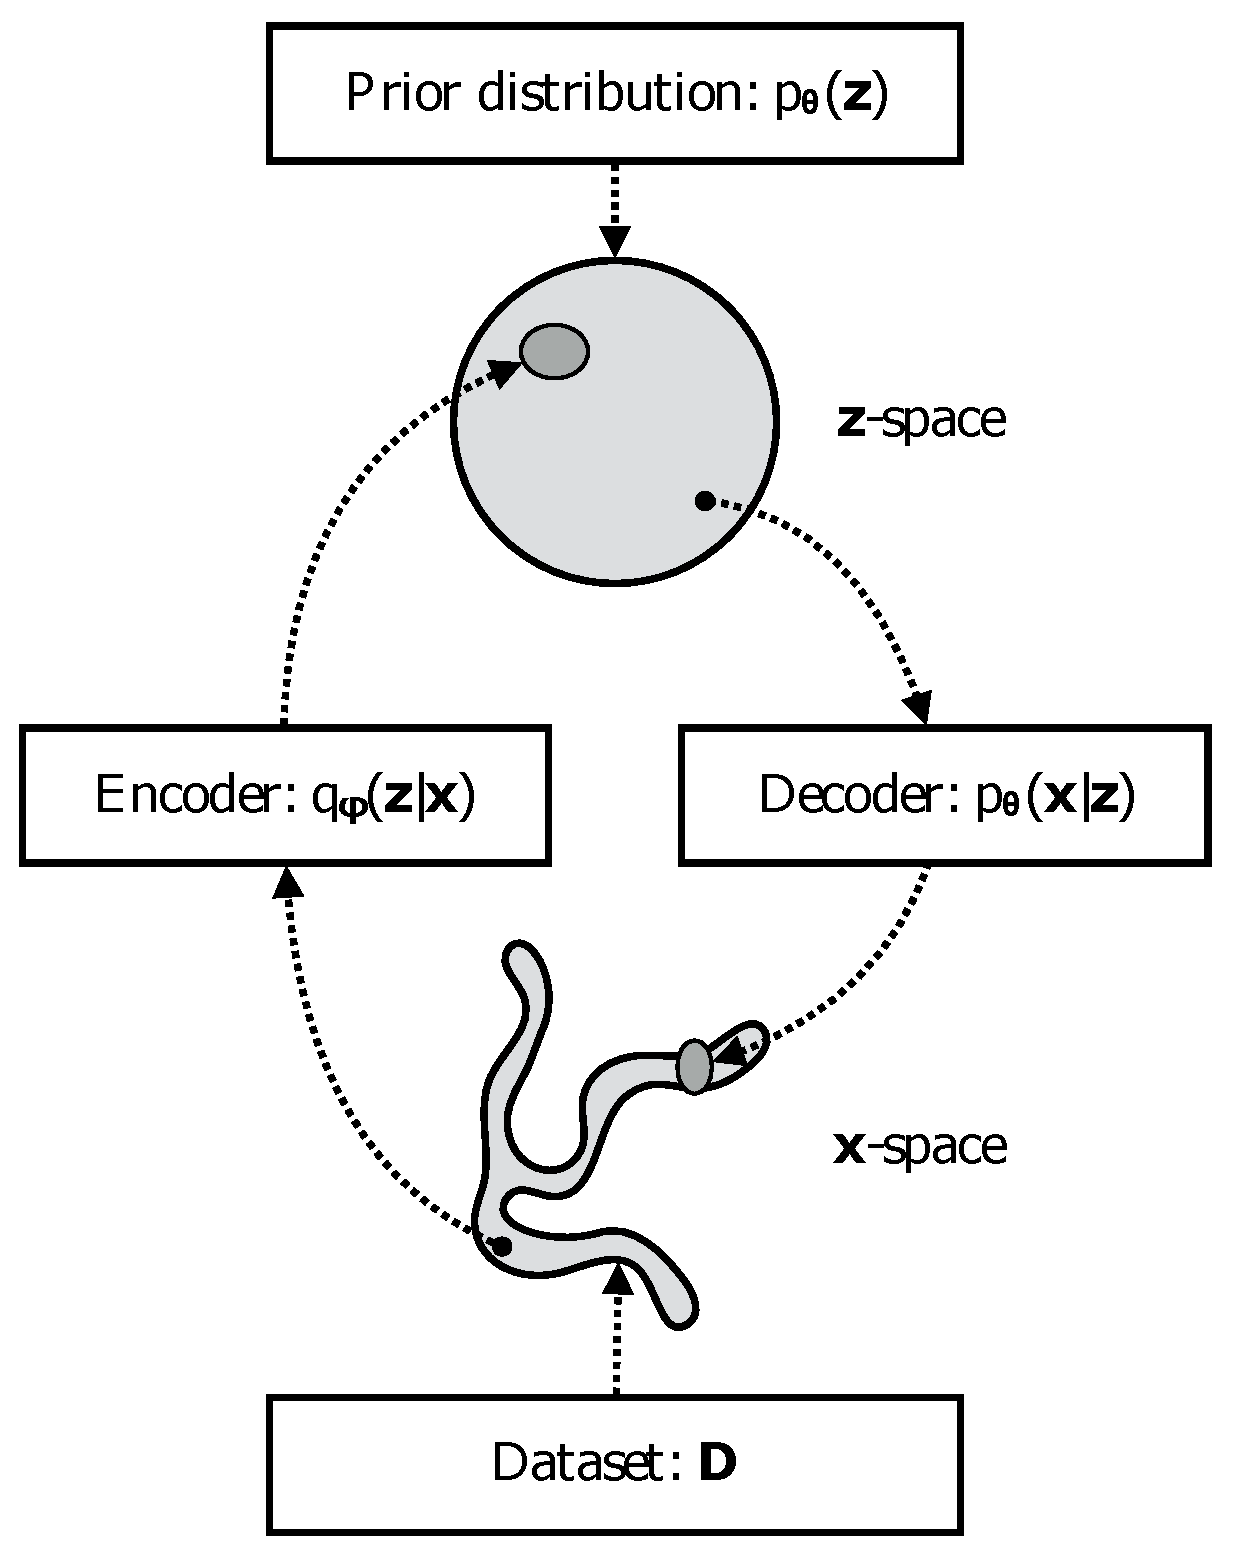
\includegraphics[width=0.5\linewidth]{figs/model/VAE.pdf}
    \caption[The variational autoencoder.]{The variational autoencoder. An
        encoder maps an observation to a probability distribution over latent representations. A sample is taken from that distribution, and a decoder
        reconstructs the observation from it. Training balances reconstruction and
        a divergence term that keeps the encoder's distribution close to a prior. By learning to map data to a distribution close to this prior,
        the model later is able to sample from the prior and decode new data. Source: \textcite{Kingma_2019}.}
    \label{fig:VAE}
\end{figure}

At generation time, we would like to sample a latent representation $z$ from the prior and decode it back to the data space. For that purpose, during training, the model learns to perform two tasks at once: first the data must be mapped to the latent space and organized somewhat similarly to the prior, but in such a way that it is also able to reconstruct the data from this mapping. This balance is achieved by maximizing the Evidence Lower Bound (ELBO) in Equation \ref{eq:elbo}:
\begin{equation}\label{eq:elbo}
    \ELBO(\theta, \phi; x) = \E_{q_\phi(z|x)}\!\bigl[\log p_\theta(x|z)\bigr] - \KL\!\bigl(q_\phi(z|x) \,\|\, p(z)\bigr).
\end{equation}

The first term is a reconstruction cost, measuring how well can the decoder recover $x$ from its latent representation. The second term, the Kullback-Leibler (KL) divergence \parencite{Kullback1951}, regularizes the encoder to stay close to the prior, ensuring the latent space is not sparse around the region of high probability mass under the prior. This ensures that sampling from $p(z)$ will land in regions where the decoder knows how to produce plausible datapoints.

This framework is adequate for reconstructing inputs and generating new data. However, in order to generate data targeting a specific condition, some adaptations need to occur.

In conditional variational auto-encoders \parencite{Sohn_Lee_Yan_2015}, a condition $c$ is presented to the decoder as a ``hint'' that guides generation, so that the model learns $p_\theta(x\mid z,c)$ rather than $p_\theta(x\mid z)$. At generation time, $z$ is still drawn from a fixed $p(z)$, and the condition acts only at decoding time. Alternatively, it is possible to condition the prior instead, letting each condition $c$ define its own region
\begin{equation*}\label{eq:cond_prior}
    p(z\mid c)=\Ncal\!\left(\mu(c),I\right),
\end{equation*}
so that data examples that are more akin to $c$ are drawn towards $\mu(c)$ during training. The latent space then acquires a geometry in which proximity to $\mu(c)$ encodes certain compatibility with $c$.

\subsubsection{The role of negative examples}
Another important consideration is that conventional conditional VAE training makes use only of positive example pairs $(c,x)$ available in the dataset. This follows naturally from the reconstruction objective: every example pair is treated as something that the model should learn to reproduce for that condition. As a consequence, a substantial part of the information contained in  the datasets may be discarded. Alternative formulations make use of this otherwise discarded information through a contrastive formulation. Different pairs are used to encourage the latent representation of a datapoint to be more compatible with conditions for which it is positive and less compatible with those for which it is negative.

\subsection{Molecular representations}
In order to process drugs in machine learning pipelines, it is necessary to somehow convert a molecule into a numerical representation. To that end, many different approaches have been proposed. In the following, we present the ones relevant for the scope of this project.

\subsubsection{Molecular fingerprints}

Molecular fingerprints are hand-tailored descriptor vectors that try to encode relevant
chemical features. They are commonly represented as binary vectors, where each active bit indicates that a particular feature is present in the molecule. Fingerprints are constructed according to predefined rules and therefore do not depend on a training dataset. Different fingerprints encode different notions of molecular similarity, depending on which aspects of the molecular structure they preserve.

Among those, circular fingerprints describe the local chemical environments surrounding each atom. Starting from an atom, its neighborhood is iteratively expanded to include atoms and bonds at increasing topological distances, and the resulting environments are mapped into fingerprint features. The Morgan fingerprints are a widely used instance of this approach \parencite{Rogers2010ECFP}. Molecules therefore receive similar fingerprints when they contain similar local substructures, even when those substructures occur in different parts of the complete molecular graph.

MACCS fingerprints, on the other hand, take a different approach. Rather than generating features from the particular molecule, they use a fixed dictionary of predefined structural keys \parencite{Durant2002MACCS}. Each key corresponds to the presence or absence of a particular structural pattern or molecular property, such as ``are there fewer than 3 oxygens?'' The resulting fingerprint records which of these predefined patterns occur in the molecule. This makes MACCS fingerprints comparatively interpretable, since individual dimensions correspond to known chemical patterns, but also limits their resolution to the structures represented by the key set.

A third kind of fingerprints, known as pharmacophore fingerprints, abstract away from the exact molecular structure. Instead of describing particular atoms or substructures, they represent features that are relevant to molecular interactions, such as hydrogen-bond donors and acceptors, aromatic groups, and charged regions. A 2D pharmacophore fingerprint additionally encodes how these interaction features are arranged within the molecular graph, using the number of bonds along the shortest paths between them rather than their physical distances in three-dimensional space \parencite{Gobbi_Poppinger_1998}. Consequently, two molecules with different atomic structures may still have similar pharmacophore fingerprints if they present comparable interaction features in similar relative arrangements. This makes pharmacophore fingerprints particularly useful when structural similarity is not required for molecules to exhibit similar biological behavior.

Finally, the RDKit fingerprint instead describes the topology of the molecular graph by enumerating subgraphs over paths of bounded length and hashing them into a fixed-length representation \parencite{Landrum_RDKit}. In contrast with Morgan fingerprints, which are centered around atoms and their neighborhoods, the RDKit fingerprint is based on paths through the molecular graph.

\subsubsection{Molecular strings}
Molecular structures can also be represented as a one-dimensional sequence of symbols. Such
representations are particularly convenient for sequence models, since a molecular
string can be tokenized and processed in the same way as other discrete
sequences.

Several molecular string representations have been proposed, differing in the rules
used to translate between a molecular graph and a sequence. This work considers two:
SMILES and SELFIES.

\paragraph{SMILES.}
The Simplified Molecular Input Line Entry System represents atoms, bonds, branches and ring closures as a string \parencite{Weininger_1988}. Several strings can describe the same molecular graph. A syntactically plausible token sequence can still violate molecular syntax or valence constraints (how many bonds an atom presents in nature). Validity must therefore be assessed after parsing.

\paragraph{SELFIES.}
Self-referencing embedded strings use a representation whose decoding rules enforce molecular constraints \parencite{Krenn_Hase_Nigam_Friederich_Aspuru-Guzik_2020}. Thus, every SELFIES sequence can be parsed as a valid molecule. This reduces failures caused by arbitrary combinations of molecular tokens.

Figure \ref{fig:notations} gives the two notations for three molecules. Ethanol is a
chain of three heavy atoms and both notations simply list them. Benzene is a ring, and
the two differ in how they close it: SMILES opens the ring with the digit \texttt{1}
and closes it with a matching \texttt{1} six atoms later, whereas SELFIES writes a
\texttt{[Ring1]} token whose argument counts back to the atom the bond returns to.
That difference is one of the reasons why SMILES strings may be invalid. In SMILES, the digit is a promise the rest of the
string has to keep, and a if generator emits just \texttt{c1ccccc}, this cannot be parsed back into a molecule.
In SELFIES, no token sequence can fail: reading is governed by
rules that track how many bonds each atom still has available, making any string over the alphabet
decodes to some valid molecule.

\begin{figure}[H]
    \centering
    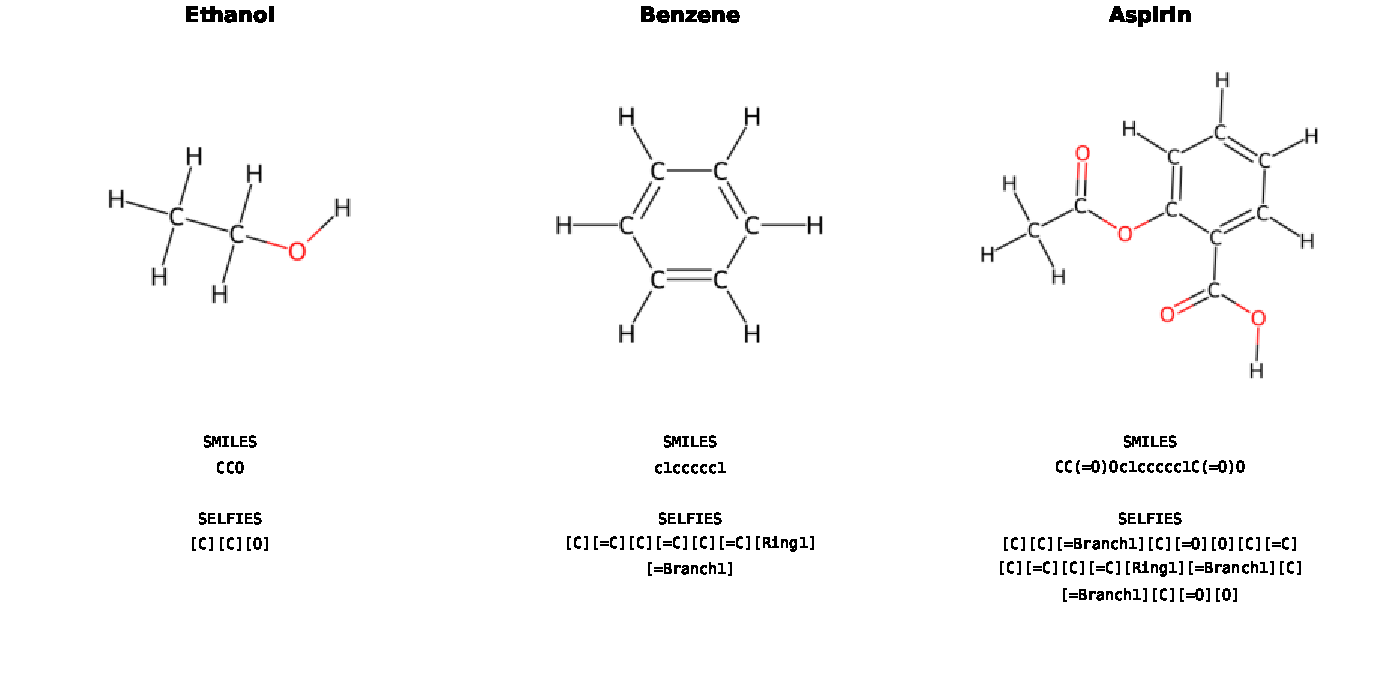
\includegraphics[width=\linewidth]{figs/model/notations.pdf}
    \caption[The same molecules in SMILES and SELFIES.]{Three molecules shown as
        structures together with the two string notations that denote them. SMILES encodes
        branches with parentheses and rings with paired digits, so the digit opening a ring
        is a commitment the remainder of the string must honor and a syntactically
        plausible string can still denote no molecule at all. SELFIES replaces this
        with bracketed tokens whose meaning is resolved against the valences still available
        as the string is read, so every sequence of tokens decodes to a valid structure.
        Both notations follow the usual convention of leaving hydrogens implicit. Those are recovered when the string is read.}
    \label{fig:notations}
\end{figure}

\subsubsection{Transformer-based representation}
Once a molecule has been written as a molecular string, it can be represented as a
sequence of discrete tokens. For example, atoms, bonds, branches and ring operations
may correspond to individual tokens depending on the notation and tokenizer employed.
A learned embedding maps each token to a continuous vector, producing a sequence of
vectors that can be processed by a neural network.

In this work, sequence-based molecular representations are learned using Transformers
\parencite{Vaswani_Shazeer_Parmar_Uszkoreit_Jones_Gomez_Kaiser_Polosukhin_2017}.
Transformers allow the representation of each token to incorporate information from
other positions in the sequence through the attention mechanism. Unlike recurrent
models, which propagate information sequentially from one position to the next,
self-attention permits direct interactions between arbitrary positions.

Let the input sequence be represented by vectors collected in a matrix $X$. For each attention head, three learned linear transformations map these vectors into query, key and value representations:
\begin{equation*}
    Q=XW_Q,\qquad K=XW_K,\qquad V=XW_V.
\end{equation*}

For a given token, its query vector describes the information it seeks from the rest of the sequence, while the key vectors describe the information associated with the other positions. Their compatibility is measured by the dot product between queries and keys. Scaled dot-product attention is therefore defined as

\begin{equation*}
    \operatorname{softmax}
    \left(
    \frac{QK^{\mathsf T}}{\sqrt{d_k}}
    \right)V,
\end{equation*}

\noindent where $d_k$ is the dimensionality of the key vectors. The matrix $QK^{\mathsf T}$ contains a compatibility score for every pair of sequence positions. The softmax operation converts the scores for each query into normalized attention weights, and the resulting weighted combination of the value vectors determines the contextual representation of that token. A token can therefore assign greater importance to positions that are particularly informative for its interpretation.

Transformers use multi-head attention, in which several attention operations are performed in parallel with different learned projections. Different heads can consequently capture different relationships between tokens. Their outputs are concatenated and projected back into the model representation. Attention layers are combined with position-wise feed-forward networks, residual connections and normalization layers to form transformer blocks.

Because attention alone does not encode the order of the tokens, positional information must also be introduced. Positional encodings are added to the token representations, allowing the model to distinguish, for example, two identical tokens appearing at different positions in a sequence.

The pattern of permitted attention depends on the task. In a transformer encoder, every position can generally attend to every other position in the input sequence, producing representations that incorporate information from the entire sequence. In an autoregressive decoder, a causal attention mask prevents position $t$ from attending to positions $t+1,t+2,\ldots$. Consequently, the representation used to predict the next token can depend only on the preceding tokens and on any additional conditioning information supplied to the model.

During training, autoregressive transformers commonly use teacher forcing. Given an observed sequence $(x_1,x_2,\ldots,x_T)$, the model receives the true preceding tokens and is trained to predict each following token. Its objective can therefore be written as maximizing

\begin{equation*}
    \prod_{t=1}^{T}
    p(x_t\mid x_{<t}),
\end{equation*}

\noindent or, for a conditional model with conditioning information $c$,

\begin{equation*}
    \prod_{t=1}^{T}
    p(x_t\mid x_{<t},c).
\end{equation*}

Generation differs from training because the true continuation is no longer available. Starting from an initial token or prefix, the model predicts a probability distribution over the next token, from which a token is selected or sampled. This token is appended to the sequence and used as part of the input for the following prediction. The procedure is repeated autoregressively until an end-of-sequence token is produced or a predefined maximum length is reached.

\subsection{Protein-targeted molecular generation}
\label{sec:protein_targeted_generation}
Early approaches explored whether molecular generation could be guided directly
from protein information. \textcite{Uludogan_Ozkirimli_Ulgen_2022}, for
example, generate molecules conditionally on different proteins and compare
their docking behavior. DeepTarget \parencite{Chen_Wang_Wang_2023} similarly
generates molecules from amino-acid sequences and evaluates them using both
learned affinity predictors and molecular docking, including experiments on
held-out proteins. More recently, several methods have proposed substantially different
architectures for protein-conditioned generation. Three of them are used as
the competitors in this work.

\paragraph{DeepDTAGen
    {\normalfont\parencite{Shah_Zhu_Lu_Wang_Tang_Li_2025}}}
combines graph-based molecular encoding, convolutional protein encoding and
variational generation. The protein sequence is processed by a gated
convolutional network, while the molecule is represented by a graph
convolutional network producing atom-level and graph-level representations.

Each molecular node representation
parameterizes a Gaussian posterior, and sampled latent representations are
modified using both the protein representation and the measured affinity.
These representations are processed by a Transformer and decoded
autoregressively into SMILES. Training jointly optimizes molecular
reconstruction, affinity prediction and Kullback-Leibler regularization. At
generation time, the molecular input is replaced by noise and the requested
protein and affinity value guide generation.

\paragraph{Prot2Drug
    {\normalfont\parencite{Creanza_Alberga_Patruno_Mangiatordi_Ancona_2025}}}
uses a simpler decoder-only formulation. A protein embedding is supplied to an
autoregressive Transformer decoder as a memory representation to which each
position in the molecular sequence can attend. The model then generates SMILES
token by token using causal self-attention. Unlike DeepDTAGen, generation does
not rely on a molecular latent variable or an auxiliary affinity-regression
objective. Conditioning is introduced directly through the protein
representation supplied to the decoder.

\paragraph{ZeroGEN
    {\normalfont\parencite{Chen_Wang_Li_Zeng_Zeng_Xu_2025}}}
combines molecular generation with protein-ligand representation learning.
Molecular pre-training first uses masked-token prediction. Joint training then
combines autoregressive molecular generation, protein-ligand contrastive
learning and interaction prediction. The contrastive objective aligns molecular
and protein representations and uses momentum-updated encoders together with a
queue of previous examples to provide a large collection of negatives.
Protein-ligand interaction prediction additionally uses hard negative pairs and
an affinity-regression objective.

These models illustrate three different strategies for incorporating protein
information into molecular generation. They therefore provide complementary
baselines for evaluating the effect of protein conditioning in the experiments
of Chapter~\ref{sec:results}.

\subsection{Selectivity-aware generation and evaluation}
\label{sec:related_selectivity}
The terminology used for selectivity is not consistent across the
literature. Terms such as ``target specificity'', ``pocket specificity''
and ``selectivity'' have been used for properties ranging from high affinity
towards a target to differences between molecular distributions generated for
different proteins. A smaller body of work has explicitly considered relative
target-versus-off-target interactions, which is the definition we assume.

One early example is CogMol
\parencite{Chenthamarakshan_Das_Hoffman_2020}. The authors distinguish target
specificity from off-target selectivity and define, for a molecule $m$ and
target $T$,
\begin{equation*}
    \operatorname{Sel}(T,m)
    =
    \operatorname{BA}(T,m)
    -
    \frac{1}{k}
    \sum_{i=1}^{k}
    \operatorname{BA}(T_i,m),
\end{equation*}
where $\operatorname{BA}$ denotes predicted binding affinity and
$T_1,\ldots,T_k$ are alternative targets. This quantity is used together with
other molecular properties to guide the search for candidate molecules in the
latent space. However, CogMol uses target-specific affinity predictors to filter generated molecules
is a post hoc manner, instead of training a generator that is itself
conditioned directly on the protein.

\textcite{Gao_Ren_Ni_2024} observed that molecules achieving
favorable docking scores against their intended pockets may also obtain
favorable scores against unrelated pockets. They therefore introduce the
$\Delta$ score, which compares the docking score of a generated molecule
against its intended pocket with its scores against alternative pockets.
Re-evaluation of several structure-based generators showed that improvements
in conventional docking scores did not necessarily correspond to improvements
in this relative measure. \textcite{Gao_Tan_Huang_2024} further showed that
docking scores produced by AutoDock Vina can be affected by molecular
properties such as molecular size. These works provide the closest
methodological precedent to the evaluation proposed here, but fail to provide a solution to the problem.

The importance of negative information during training has also received
attention. ConGen \parencite{Koban_Uludogan_Ozkirimli_2026} observes that
training only from known interacting drug-protein pairs provides information
about which molecules should be associated with a protein but little
information about which should not. The model therefore incorporates
non-interacting pairs through contrastive learning. Its evaluation includes
protein-level distributional measures such as Fréchet ChemNet Distance between
generated molecules and known ligands. It therefore exploits negative
drug-protein information during training, but does not directly evaluate the
relative affinity of each generated molecule towards its target and
alternative proteins.

Other studies have addressed selectivity for particular target pairs.
CMD-GEN \parencite{Zou_Guo_Fu_2025}, for example, generates molecules intended
to be selective for the protein PARP1 over PARP2 and evaluates selected candidates using
molecular dynamics, free-energy calculations and experimental measurements. This provides strong evidence that
generative methods can produce selective molecules, but only for a predefined
pair of targets rather than as a general property of a generator conditioned
on arbitrary proteins.

Recent benchmarks have also investigated whether target-aware generators
capture target-dependent chemical constraints. TarPass
\parencite{Qin_Chen_Li_2026} compares molecular distributions generated for
different proteins using Fréchet ChemNet Distance, and includes a discrimination experiment between the proteins JAK2
and TYK2. These experiments provide evidence about target-dependent generation,
but direct relative-affinity comparisons remain restricted to selected target
pairs rather than being applied systematically.

The distinction is also visible in DBMol
\parencite{Qin_Yi_Cretu_2026}, where generated molecules are described as
high-affinity and target-specific. Specificity is evaluated through quantities
including pocket coverage, interface confidence and predicted affinity, all of
which characterize compatibility with the intended binding pocket. These
criteria do not, however, require the same generated molecule to be compared
against alternative proteins.

Taken together, these works establish several complementary notions of
target-aware molecular generation: direct conditioning on protein information,
similarity to target-specific ligand distributions, interaction with a desired
binding pocket, and relative affinity against alternative targets. Relative
target-versus-off-target affinity is therefore not itself a new concept.
What remains comparatively less explored is its use as a systematic diagnostic
of protein-conditioned generators across arbitrary target proteins.

Throughout this work, for each generated molecule, the
conditioning protein is compared against a common panel of alternative
proteins, allowing target preference to be studied at the level of the
generator instead of only for selected target pairs. Chapter~\ref{sec:metrics}
formalizes this evaluation and introduces complementary metrics for measuring
different aspects of selective generation.

\chapteropening
{Metrics}
{figs/chapters/metrics.pdf}
{0.85\textwidth}
{Geometric interpretation of utility. In its most general sense, a generator is selective if the drugs it generates have higher affinity values for the proteins they were designed for than for other proteins. $p_G$ is the distribution of on-target affinities, and $q_G$ is the distribution of off-target affinities. If we measure the difference in the areas of each curve above a biologically relevant threshold $\tau$, we get a value called utility. We show in Proposition \ref{prop:delta} that integrating this utility over all possible $\tau$ values yields the $\Delta$ score discussed previously.}
{%
    \lettrine[
        lines=2,
        lhang=0.0,
        loversize=0.0
    ]{L}{}\textit{ike any comparison, selectivity cannot be read from a single affinity
        value. However, there are many ways in which a model can appear to be selective while
        failing to truly separate on-target and off-target affinities. This chapter
        defines this quantity, and then the diagnostics to measure its different aspects.}
}
[Man is the measure of all things: of the things that are, that they are, of the things that are not, that they are not.]
[Protagoras of Abdera][sec:metrics][Geometric interpretation of utility.][fig:metrics]

\subsection{Problem statement}\label{sec:defs}
Let $\mathfrak D=\{\mathfrak d_1,\ldots,\mathfrak d_M\}$ be a set of molecules and $P=\{p_1,\ldots,p_N\}$ a set of proteins. A dataset is a partially observed matrix $\mathcal{D} \in \mathbb{R}^{M\times N}$, where $\mathcal{D}_{m,n}$ is the affinity value for the drug-protein pair $(\mathfrak{d}_m, p_n)$ if it was experimentally observed, or an unobserved entry otherwise. Each dataset also carries an affinity threshold $\tau$ that is dependent on the experimental conditions of the data collection. An observation is said to be positive (the drug and the protein do bind) if $\mathcal D_{m,n}\geq \tau$.

A stochastic generator $G_\omega$ with parameters $\omega$ receives a protein $p_i$ and proposes $K$ molecules for it, independently drawn from $G_\omega(\ \cdot\ |\ p_i)$. Since the generator may suggest the same molecule multiple times, this collection for each protein is a multiset $D_i=[d_{i,1},\ldots,d_{i,K}]$. In order to evaluate the proposed molecules, a regressor model called an affinity ``oracle'' $f_\theta$ is trained on the dataset to predict the affinity between drug-protein pairs. The oracle estimates
$A_{i,k}^{(j)}=f_\theta(d_{i,k},p_j)$, the predicted affinity between drug $d_{i,k}$ and protein $p_j$.

The set
\begin{equation*}
    \mathcal{A}_{on}=\left\{ A_{i,k}^{(i)} \right\}_{i,k}
\end{equation*}
contains the on-target predicted affinities, \emph{i.e.}, affinities between drugs and the proteins for which they were created. In the same way, the set
\begin{equation*}
    \mathcal{A}_{off}=\left\{ A_{i,k}^{(j)}\right\}_{i,j,k;\, j \neq i}
\end{equation*}
contains off-target predicted affinity values, \emph{i.e.}, between a drug and a protein the drug is not intended to bind. For a sufficiently big number of generated molecules, the empirical distribution of these sets can be said to approximate probability measures on the affinity space induced by the generator:
\begin{equation*}
    \mathcal{A}_{on} \sim p_G(x), \qquad\mathcal{A}_{off} \sim q_G(x).
\end{equation*}

\paragraph{Selective protein-targeted molecular generation.}

The selectivity utility of a generator $G_\omega$ is defined as
\begin{equation*}
    U(G_\omega, \tau)
    =
    \mathop{\mathbb P}\limits_{X\sim p_G}(X\geq\tau)
    -
    \mathop{\mathbb P}\limits_{X\sim q_G}(X\geq\tau)
    =
    \int_\tau^\infty
    \bigl(p_G(x)-q_G(x)\bigr)\,dx.
\end{equation*}

A generator is said to be selective if $U(G_\omega, \tau)>0$, meaning that
above-threshold affinities occur more frequently for target proteins
than for off-target proteins. The problem of selective protein-targeted
molecular generation is to find an architecture for $G_\omega$ and a
training scheme for $\omega$ that maximize this utility.

We next define how to explore possible blind spots of this notion and introduce complementary metrics to diagnose it. Before, however, it is necessary to define three general metrics of quality: validity, uniqueness and novelty.

\subsection{Generation quality metrics}
These metrics quantify the overall quality of a molecular generator. Ideally, such a model should produce valid drugs (\emph{i.e.}, strings that can be interpreted as real physical molecules, such as ``CCCOC'', instead of ``C(.(/+\textbackslash)c@OC''). Another property of interest is uniqueness, \emph{i.e.}, the model should produce diverse outputs, instead of repeating the same answers continuously. Finally, the model should extrapolate beyond the drugs observed in the training set, suggesting novel compounds. Let $[a, a, b, ...]$ be a multiset, \emph{i.e.}, a set admitting repeated elements, and the operator $|.|$ be the cardinality of a set or multiset.

\paragraph{Validity} is the fraction of structurally valid molecules.\\
\begin{equation}
    \text{Validity}=\dfrac{|\left[d_{i,k}:d_{i,k}\text{ is a valid molecule}\right]|}{|\left[d_{i,k}\right]|}
\end{equation}

\paragraph{Uniqueness} is the proportion of unique molecules generated. Penalizes repetitive generation.
\begin{equation}
    \text{Uniqueness}=\dfrac{|\left\{d_{i,k}\right\}|}{|\left[d_{i,k}\right]|}
\end{equation}

\paragraph{Novelty} is the percentage of generated drugs that weren't present in the training data. Incentivizes generalizing beyond the observed examples.
\begin{equation}
    \text{Novelty}=\dfrac{|\{d_{i,k}:d_{i,k}\notin\mathcal{D}_\text{train}\}|}{|\left[d_{i,k}\right]|}
\end{equation}

\subsection{Selectivity metrics}
Building upon the notion of utility discussed in Section \ref{sec:defs}, the following metrics characterize complementary aspects of selective generation. The $\Delta$ score measures the magnitude of the on-target affinity advantage, Distributional $\Delta$ measures separation between the complete affinity distributions, Directional Consistency measures how frequently individual comparisons have the desired ordering, and the Tanimoto Gap tests whether the conditioning protein also induces a structural change in the generated chemical space. Effective $\Delta$ additionally combines selectivity with generation quality and is consequently used as the primary criterion for model selection.

\paragraph{$\Delta$ score {\normalfont\parencite{Gao_Ren_Ni_2024}}}
measures whether a molecule generated for a target protein is predicted to bind more strongly to that protein than to alternative proteins. For each molecule $d_{i,k}$ generated conditionally on protein $p_i$, its individual $\delta$ is defined as the difference between its on-target affinity and its mean affinity with all off-target proteins, as seen in Equation \ref{eq:delta}. This quantity $\delta(\ \cdot\ )$ looks at individual generated molecules.

\begin{equation}\label{eq:delta}
    \delta(d_{i,k})
    =
    A_{i,k}^{(i)}
    -
    \frac{1}{N-1}
    \sum_{j\neq i}
    A_{i,k}^{(j)}.
\end{equation}

The overall $\Delta$ score is obtained by averaging this quantity across all generated molecules and target proteins:

\begin{equation*}
    \Delta
    =
    \frac{1}{NK}
    \sum_{i=1}^{N}
    \sum_{k=1}^{K}
    \delta(d_{i,k}).
\end{equation*}

The metric takes values in $\mathbb{R}$ and is expressed in the same units as the affinity measure. A value of $\Delta=0$ indicates, on average, no preference for the conditioning protein over the off-target proteins, while positive values indicate greater predicted affinity for the conditioning target. Higher values are therefore desirable.

An important result is that the $\Delta$ score can be derived as an aggregate, $\tau$-independent utility, as stated in Proposition \ref{prop:delta}.

\begin{proposition}
    \label{prop:delta}
    Assume that the on-target and off-target affinity random variables take
    values in a bounded interval $[a,b]$. Then, in the population limit, the
    $\Delta$ score is the signed area under the threshold-dependent utility
    curve:
    \begin{equation*}
        \Delta
        \overset{K\rightarrow\infty}{\longrightarrow}
        \Delta_G
        =
        \int_{-\infty}^{\infty}
        U(G_\omega,t)\,dt.
    \end{equation*}
\end{proposition}

\begin{proof}
    Let $X\sim p_G$ and $Y\sim q_G$. For any $x,y\in[a,b]$,
    \begin{equation*}
        x-y
        =
        \int_{-\infty}^{\infty}
        \left(
        \mathds{1}[x\geq t]
        -
        \mathds{1}[y\geq t]
        \right)dt.
    \end{equation*}
    Indeed, if $x>y$, the integrand is equal to one on $(y,x]$ and zero
elsewhere, so the integral is $x-y$. The case $x<y$ is analogous.

As $K\rightarrow\infty$, the empirical $\Delta$ score converges to
\begin{equation*}
    \Delta_G
    =
    \underset{X\sim p_G}{\mathbb E}[X]
    -
    \underset{Y\sim q_G}{\mathbb E}[Y].
\end{equation*}

Since $X,Y\in[a,b]$, the function
\begin{equation*}
    \mathds{1}[X\geq t]-\mathds{1}[Y\geq t]
\end{equation*}
vanishes outside $[a,b]$ and is bounded in absolute value by one.
It is therefore integrable, and Fubini's theorem gives
\begin{align*}
    \Delta_G
    &=
    \mathbb E[X-Y]
    \\
    &=
    \int_{-\infty}^{\infty}
    \mathbb E
    \left[
        \mathds{1}[X\geq t]
        -
        \mathds{1}[Y\geq t]
        \right]dt
    \\
    &=
    \int_{-\infty}^{\infty}
    \left(
    \underset{X\sim p_G}{\mathbb P}(X\geq t)
    -
    \underset{Y\sim q_G}{\mathbb P}(Y\geq t)
    \right)dt
    \\
    &=
    \int_{-\infty}^{\infty}
    U(G_\omega,t)\,dt.
    \qedhere
\end{align*}
\end{proof}

\medskip

This geometric relationship is expressed in Figure \ref{fig:metrics}.

The $\Delta$ score may overlook some problems in the generation process. We extend it to also consider different failure points.

\paragraph{Effective $\Delta$ score} measures a balance between selectivity and generation quality, in order to assess an average $\Delta$ score per generation attempt. A model may present a high $\Delta$ score by simply memorizing the best example in the dataset and repeating it, or by making drugs with very low off-target affinity but low on-target affinity. The effective $\Delta$ score measures this by assigning zero contribution to outputs that fail the validity, uniqueness, novelty, or on-target affinity requirements:
\begin{equation*}
    \begin{gathered}
        S = \left\{\, d_{i,k} :
        d_{i,k} \text{ is valid, unique, novel, and }
        A_{i,k}^{(i)} \geq \tau \,\right\}, \\
        \text{Effective }\Delta
        = \frac{1}{NK}
        \sum_{i=1}^{N}\sum_{k=1}^{K}
        \delta(d_{i,k})\,
        \mathds{1}\!\left[d_{i,k}\in S\right].
    \end{gathered}
\end{equation*}

The Effective $\Delta$ score takes values in $\mathbb{R}$, with zero representing no net selective contribution and higher values being desirable.

\paragraph{Distributional $\Delta$ score}
considers not only the difference between the means of the on-target and off-target affinity distributions, but also their dispersion. A model may have very high separation in the means of the on-target and off-target affinity distributions while presenting high dispersion, with significant overlap in those distributions. Consider again the empirical samples $\mathcal{A}_{on}$ and $\mathcal{A}_{off}$ corresponding respectively to the on-target and off-target predicted affinities. A univariate Gaussian distribution is fitted by maximum likelihood to each sample:
\begin{equation*}
    P = \mathcal{N}(\mu_{on},\sigma_{on}^2),
    \qquad
    Q = \mathcal{N}(\mu_{off},\sigma_{off}^2).
\end{equation*}

The separation between the two fitted distributions is quantified using the Kullback-Leibler divergence. Since the KL divergence is non-negative and does not encode the direction of the affinity difference, its sign is determined by the difference between the corresponding means. The Distributional $\Delta$ score is therefore defined as

\begin{equation*}
    \text{Distributional }\Delta
    =
    \operatorname{sign}(\mu_{on}-\mu_{off})\,
    D_{\mathrm{KL}}\!\left(P\,\|\,Q\right).
\end{equation*}

The metric takes values in $\mathbb{R}$. A value of zero indicates no separation between the fitted distributions, while positive values indicate that the on-target affinity distribution is shifted towards higher affinities than the off-target distribution. Higher values are desirable.

\paragraph{Directional Consistency}
is an outlier-robust evaluation. It measures the frequency with which the predicted on-target affinity is greater than the corresponding off-target affinity. A high $\Delta$ score can be achieved by generating one extremely selective drug, but such a generator would achieve a low directional consistency. Importantly, this metric can be used to evaluate oracles, by considering the percentage of times they correctly order two proteins' affinities to a reference drug.

For each conditioning protein $p_i$, define $m(i)$ as the number of times the drugs generated for $p_i$ have an affinity higher for $p_i$ than for other proteins:
\begin{equation*}
    m(i)
    =
    \frac{1}{K(N-1)}
    \sum_{k=1}^{K}
    \sum_{j\neq i}
    \mathds{1}\!\left[
        A_{i,k}^{(i)}
        >
        A_{i,k}^{(j)}
        \right].
\end{equation*}

The overall score is obtained by averaging across target proteins:

\begin{equation*}
    \text{Directional Consistency}
    =
    \frac{1}{N}
    \sum_{i=1}^{N}
    m(i).
\end{equation*}

Directional Consistency lies in $[0,1]$. A value of $1$ indicates that every generated molecule is predicted to have greater affinity for its conditioning protein than for every off-target protein, whereas a value of $0$ indicates the opposite ordering in every comparison. A value of $0.5$ corresponds to chance-level directional consistency, with no systematic preference for the conditioning protein. Higher values are desirable.

\paragraph{Tanimoto Gap}
evaluates whether molecules generated for the same conditioning protein are more structurally similar to one another than to molecules generated for different proteins. This is the only metric that is unrelated to affinity, measuring only conditioning effects on the chemical space.

For each protein $p_i$, the average within-target molecular similarity is defined as
\begin{equation*}
    g_{\mathrm{within}}(i)
    =
    \frac{1}{K(K-1)}
    \sum_{k=1}^{K}
    \sum_{\ell\neq k}
    T\!\left(
    M(d_{i,k}),
    M(d_{i,\ell})
    \right).
\end{equation*}

The corresponding cross-target similarity compares molecules generated for $p_i$ with molecules generated for every other conditioning protein:
\begin{equation*}
    g_{\mathrm{cross}}(i)
    =
    \frac{1}{K^2(N-1)}
    \sum_{k=1}^{K}
    \sum_{j\neq i}
    \sum_{\ell=1}^{K}
    T\!\left(
    M(d_{i,k}),
    M(d_{j,\ell})
    \right).
\end{equation*}

The Tanimoto Gap is then defined as

\begin{equation*}
    \text{Tanimoto Gap}
    =
    \frac{1}{N}
    \sum_{i=1}^{N}
    \left[
        g_{\mathrm{within}}(i)
        -
        g_{\mathrm{cross}}(i)
        \right].
\end{equation*}

The metric lies in $[-1,1]$. Positive values indicate that molecules generated for the same protein are, on average, more structurally similar to one another than to molecules generated for different proteins. A value of zero indicates no systematic difference between within-target and cross-target similarities, while negative values indicate greater similarity across targets than within targets. Higher values are desirable.

\subsection{Chemical quality metrics}
Finally, this set of metric tries to capture if the generated molecules are ``reasonable'' in a chemical sense. This intuition has been operationalized in different ways over the years.

\paragraph{Mean predicted affinity} is average predicted affinity value given by the oracle for all generated drugs with their respective targets, measured as $A_{i,k}^{(i)}$.

\paragraph{Mean of the top decile} measures the same, but considering only the $10 \%$ drugs with the highest predicted affinities, so as to evaluate a model on its best.

\paragraph{Success rate} is the percentage of generated drugs with predicted affinity above the dataset's threshold and that are both unique and novel.

\paragraph{Fréchet ChemNet distance (FCD) {\normalfont\parencite{Preuer2018FCD}}.} Similar to the Fréchet Inception Distance \parencite{Heusel2017FID}, which uses a pre-trained benchmark Inception-v3 model \parencite{Szegedy2016Inception} to generate embeddings for a set of real images and for a set of images generated by the model being evaluated. The purpose is to measure if the extracted semantics present in the embeddings follow the same distribution. In this case, the comparison is done against the ChemNet model \parencite{Goh2018ChemNet}, and calculated as the 2-Wasserstein distance of the distributions (which are assumed to be approximately Gaussian) of the embeddings of real examples ($r$) and generated ones ($g$):

\begin{equation*}\label{eq:fcd}
    \text{FCD} = \|\bm{m}_g - \bm{m}_r\|_2^2 + \text{Tr}\!\left(\bm{\Sigma}_g   - 2\left(\bm{\Sigma}_g \bm{\Sigma}_r\right)^{1/2}+ \bm{\Sigma}_r\right),
\end{equation*}
where $\bm{m}$ and $\bm{\Sigma}$ are the mean and covariance matrices.

\paragraph{Internal diversity {\normalfont\parencite{Polykovskiy2020MOSES}}} is the average pairwise Tanimoto distance computed over the Morgan fingerprints of the generated set of molecules. Let $M(d_{i, k})$ be the Morgan fingerprint of drug $d_{i, k}$, and $T(v, w) = \dfrac{v^T w}{v^Tv + w^Tw -v^Tw}$ the tanimoto similarity between two binary vectors $v$ and $w$. Then,
\begin{equation*}
    \text{Internal diversity}=1-\dfrac{1}{NK(K-1)}\sum_{i=1}^N\sum_{k=1}^K\sum_{\ell\neq k} \text{T}(\text{M}(d_{i,k}),\text{M}(d_{i,\ell})).
\end{equation*}

\paragraph{Lipinski’s rule of five (Ro5) {\normalfont\parencite{Lipinski1997}}.} Evaluates ``druglikeness'' and helps to determine if a chemical compound has properties that would make it a likely orally absorbable drug in humans. A molecule is likely to be poorly absorbed if it violates more than one of the following criteria:

\begin{itemize}
    \item Molecular mass inferior to $500$ Da.
    \item An octanol-water partition coefficient ($\log P$) inferior to $5$.
    \item No more than $5$ hydrogen bond donors (expressed as the sum of OH and NH groups).
    \item No more than $10$ hydrogen bond acceptors (expressed as the sum of N and O atoms).
\end{itemize}

The final score is the percentage of drugs that don't violate more than one of the criteria.

\paragraph{Quantitative estimate of drug-likeness (QED) {\normalfont\parencite{Bickerton2012QED}}.} Like Ro5, calculates several properties to measure the ``beauty'' of a molecule in a pharmacological sense defined in the original paper. Ranges from 0 (completely non-druglike) to 1 (highly druglike).

\paragraph{Synthetic accessibility score (SA) {\normalfont\parencite{Ertl2009SA}}.} Estimates the difficulty of synthesizing a given molecule. Penalizes molecules that are chemically impossible or prohibitively expensive to build in a lab. Ranges from 1 (very easy to synthesize) to 10 (very difficult to synthesize). It is calculated based on two main components: a fragment score and a complexity penalty. The fragment score analyzes how common the structural fragments composing a molecule are. If a molecule is composed of fragments frequently seen in chemical databases, it is deemed easier to synthesize. Meanwhile, the complexity penalty penalizes features that complicate synthesis, such as large rings, a high numbers of chiral centers and non-standard ring fusions.

Having clearly defined the task and the objective being optimized, the following chapter introduces the set of oracles used to predict binding affinity, an architecture for $G_\omega$ and a set of
training objectives for $\omega$ intended to increase this separation directly, without
using the oracles anywhere in the training loop.

\chapteropening
{Methods}
{figs/chapters/methods.pdf}
{0.85\textwidth}
{Variational drug encoding. A molecule is represented by a Gaussian distribution whose mean and variance are obtained from its chemical structure. Each protein defines another Gaussian in the same latent space, with a learned mean and fixed variance. Training places molecules closer to proteins for which their measured affinity is higher and further from those for which it is lower. Generation then samples from the region associated with the requested protein and decodes the sample into a molecule.}
{%
    \lettrine[
        lines=2,
        lhang=0.0,
        loversize=0.0
    ]{T}{}\textit{he model proposed in this work, SelVAEGen, learns where molecules should lie
        relative to proteins in a shared latent space, (Figure \ref{fig:drug_latent}). A molecule should lie closer to a protein it binds
        strongly than to one it binds weakly. To generate a molecule for a requested
        protein, the model samples near that protein and decodes the sample into a
        chemical structure. This chapter describes the affinity oracles used for
        evaluation, the model architecture, and the objectives that incentivize the model to learn these
        relationships.}
}[Give me a lever and a place to stand and I will move the world.][Archimedes of Syracuse][sec:methods][Variational drug encoding.][fig:drug_latent]

\subsection{Oracles}
For a newly generated molecule, experimental affinity measurements are unavailable. Evaluating whether it prefers its intended protein therefore requires estimates of its affinity to both that protein and the alternatives. We use three drug-target affinity prediction models, referred to as ``oracles'', to obtain these estimates.

\paragraph{GraphDTA {\normalfont\parencite{Nguyen_Le_Quinn_Nguyen_Le_Venkatesh_2020}}} represents the molecule through a sequence of graph attention and graph convolution layers. It represents the protein through one-dimensional convolutions over its amino-acid sequence. The two representations are concatenated and passed to a multilayer perceptron (MLP), which predicts the affinity of the pair.

\paragraph{GSDTA {\normalfont\parencite{Luo_Zhu_Xu_Xiao_Wei_Shen_2025}}} also uses graph attention followed by graph convolutions to represent the molecule. Its protein branch combines a one-dimensional convolution, a bidirectional LSTM, and a Transformer encoder. As in GraphDTA, an MLP receives the concatenated drug and protein representations and predicts their affinity.

\paragraph{Baseline.} A simpler oracle is included as a sanity check. It concatenates the molecular fingerprint representation described in Section \ref{sec:model} with the PCA-compressed ESM-C protein embedding \parencite{ESMTeam2024} and passes the result to a three-layer MLP.

GraphDTA and GSDTA use similar molecular encoders and both learn from protein sequences. The baseline provides a different representation of each input, allowing us to examine how much the predictions depend on the oracle architecture. Their disagreement is discussed in Section \ref{sec:oracles}. Unless otherwise stated, each reported affinity prediction is the average of the three oracle predictions.

\subsection{SelVAEGen}\label{sec:overview}\label{sec:varmod}\label{sec:model}

SelVAEGen has three parts, shown in Figure \ref{fig:model}. A protein encoder maps an amino-acid sequence to a vector. A drug encoder maps a molecular structure to a Gaussian distribution in the same latent space. A drug decoder receives a sample from this space together with the protein vector and produces a molecular string.

The shared space provides a way to express the relative affinities discussed in Chapter \ref{sec:metrics}. Consider a molecule measured against two proteins. If it binds one more strongly, training should place its representation closer to that protein than to the other. Likewise, among two molecules measured against the same protein, the stronger binder should lie closer to it. The model is therefore trained to make relative proximity reflect relative affinity. Sampling near a protein is then intended to produce molecules compatible with that protein.

During training, the latent representation $z$ is sampled from the molecular posterior and used to reconstruct the input molecule. During generation, it is instead sampled from the protein-conditioned prior. The decoder receives $z$ together with the protein representation in both cases.

\begin{figure}[H]

    \centering

    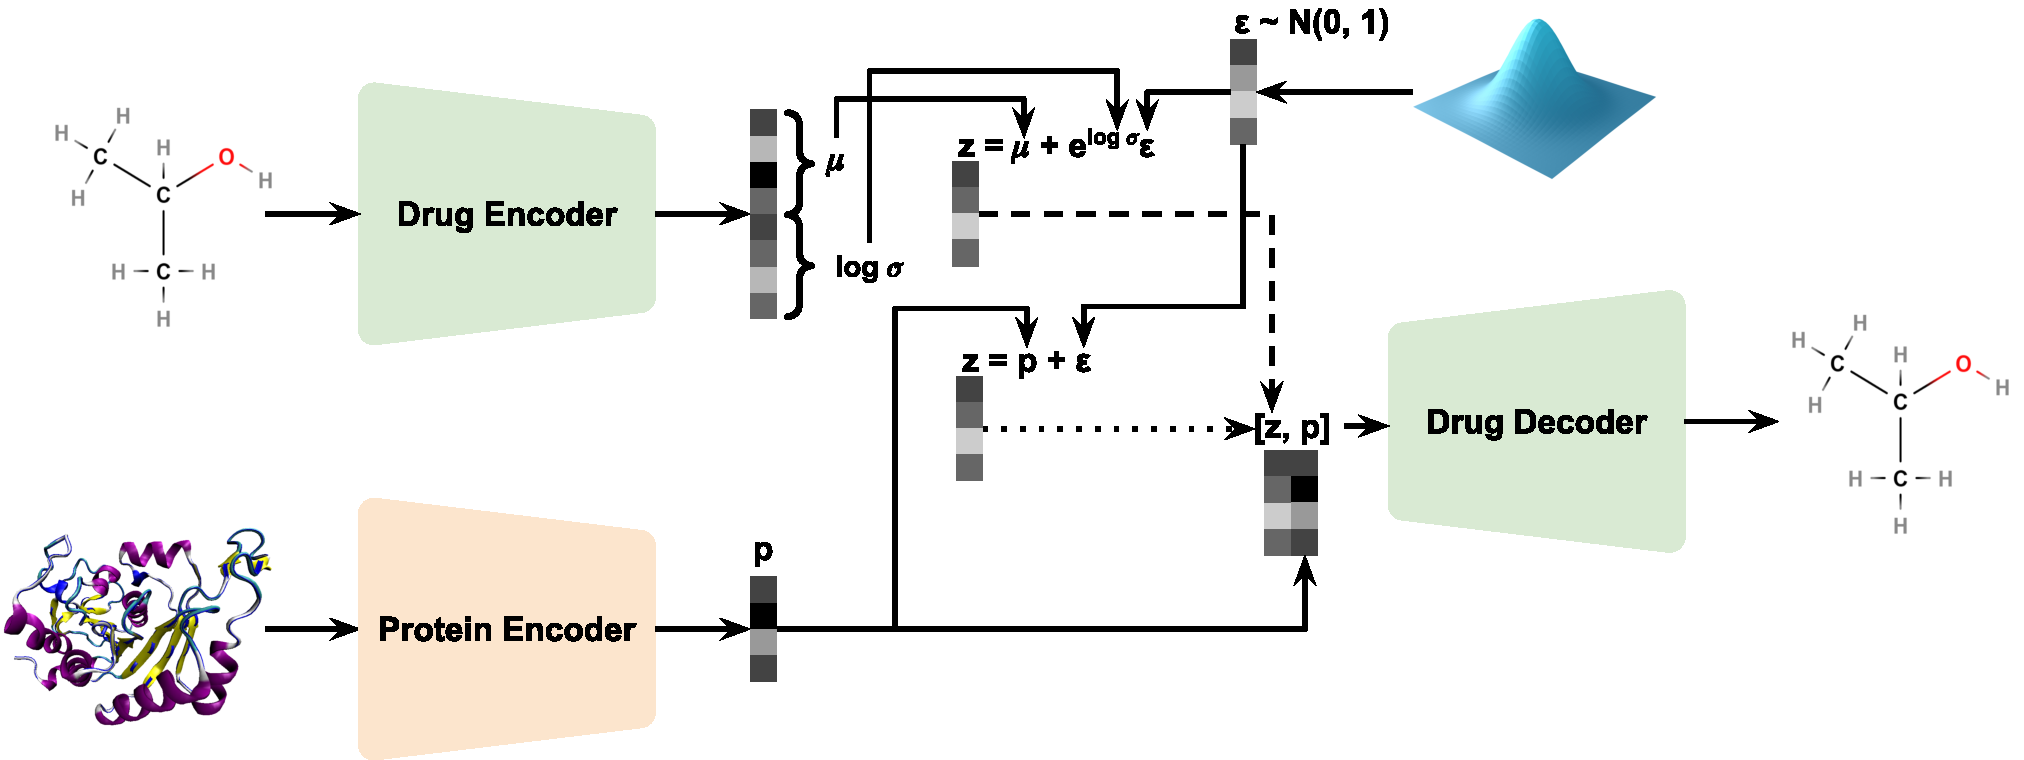
\includegraphics[width=\linewidth]{figs/model/model.pdf}

    \caption[Model overview.]{The complete SelVAEGen architecture. During training, the drug encoder supplies a posterior sample $z$ (dashed arrow) and the decoder reconstructs the input molecule. During generation, the drug encoder is unused and $z$ is sampled from the protein-conditioned prior (dotted arrow). The decoder receives the latent sample and protein representation in both cases.}

    \label{fig:model}

\end{figure}

\paragraph{Protein encoder.}

We use a pretrained protein representation so that the model can begin with information learned from protein sequences. As shown in Figure \ref{fig:protein_encoder}, a frozen ESM-C 600M model \parencite{ESMTeam2024} produces an embedding for each residue. These embeddings are averaged into a 1,152-dimensional vector, standardized coordinate-wise, and reduced to 128 dimensions by Principal Component Analysis (PCA). The resulting frozen representation is $e(P)$. A residual adapter then maps it to the prior mean $m_\psi(P)$.

The protein prior and the molecular posterior occupy the same space, so choosing the protein representation's size also fixes the latent dimensionality. The choice of 128 components retains between $89.4\%$ and $99.0\%$ of the variance of the averaged embeddings, depending on the dataset, while limiting the dimensionality of the prior regularization problem.

\begin{figure}[H]

    \centering

    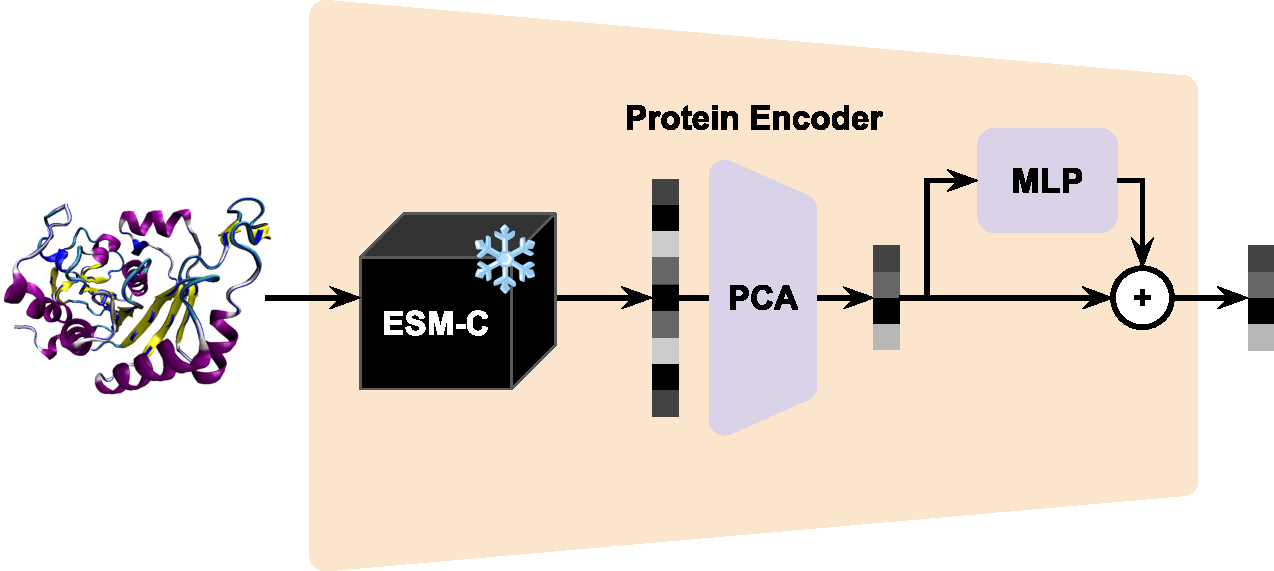
\includegraphics[width=0.72\linewidth]{figs/model/protein_encoder.pdf}

    \caption[The protein encoder.]{The protein encoder. A frozen ESM-C model produces residue embeddings, which are averaged, standardized, and reduced by PCA to the fixed representation $e(P)$. A residual adapter maps this representation to the protein prior mean $m_\psi(P)$.}

    \label{fig:protein_encoder}

\end{figure}

The protein representation determines the center of a Gaussian prior in the shared latent space:
\begin{equation*}
    p_\psi(z\mid P)
    =
    \Ncal\!\left(
    m_\psi(P),
    I
    \right).
\end{equation*}

The identity covariance $I$ fixes the protein prior's variance. Its mean $m_\psi(P)$ is obtained from the preprocessed protein representation $e(P)$ through a two-layer residual adapter:
\begin{equation*}
    m_\psi(P)
    =
    e(P)
    +
    W_2
    \operatorname{GELU}
    \left(
    W_1 e(P)+b_1
    \right)
    +b_2.
\end{equation*}

The adapter's hidden layer has 256 units. The residual connection allows it to refine $e(P)$ while retaining the pretrained representation as its starting point. Its final layer is initialized to zero, so initially $m_\psi(P)=e(P)$ exactly. Protein positions therefore begin with the arrangement supplied by the pretrained embeddings and move as the training objective requires.

The adapter is frozen for the first ten epochs and optimized jointly with the rest of the model afterwards. At the start of training, molecular posteriors carry little information. Keeping the protein positions fixed during these first epochs gives the drug encoder time to learn relative to stable reference points rather than allowing both representations to move together immediately.

\paragraph{Molecular fingerprints.}

The molecular encoder combines fingerprints with a learned representation of the molecular sequence. The fixed molecular representation concatenates four fingerprints: Morgan, MACCS, RDKit path-based, and two-dimensional pharmacophore fingerprints. These describe the complementary aspects of molecular structure introduced in Chapter \ref{sec:literature}. Morgan uses radius two. Morgan, RDKit, and pharmacophore fingerprints each contain 2,048 positions, while MACCS contains 167. PCA reduces the concatenated vector to 512 dimensions.

The fingerprint PCA projection is fitted once and reused for subsequent molecules, including generated ones. This combined representation is an input to the model. The Tanimoto metrics defined in Chapter \ref{sec:metrics} instead use the separate 2,048-bit Morgan fingerprints.

\paragraph{Drug encoder.}

Figure \ref{fig:encoder} follows the encoding of 2-propanol. The 512-dimensional fingerprint representation contributes one vector for the whole molecule. The sequence branch reads its molecular string, shown here as the SELFIES \texttt{[C][C][Branch1][C][C][O]}, using a bidirectional Transformer with sinusoidal positional encodings. It contributes one state per token.

A fusion block brings these representations together. First, token states are projected to the fingerprint vector's dimensionality, and a learned identifier is added to each representation to indicate its source. A two-layer Transformer then attends jointly over the fingerprint vector and all token states. This allows the fingerprint representation to incorporate information from individual sequence positions. Its final state is projected into $\mu_d$ and $\log\sigma_d^2$, which parameterize the molecular posterior. Using the fingerprint position gives the model a fixed place from which to read these parameters for molecules of any sequence length.

We also constructed a graph branch in which three residual GATv2 layers \parencite{Brody_Alon_Yahav_2022} with four attention heads process atoms and bonds. Its atom states enter the same fusion block. The architecture ablation compares configurations labeled sequence, graph, and both, according to which learned branches accompany the fingerprint. The graph branch gave no advantage and is omitted from the reported model. The comparison and the figures for this variant are provided in the appendix.

\begin{figure}[ht]

    \centering

    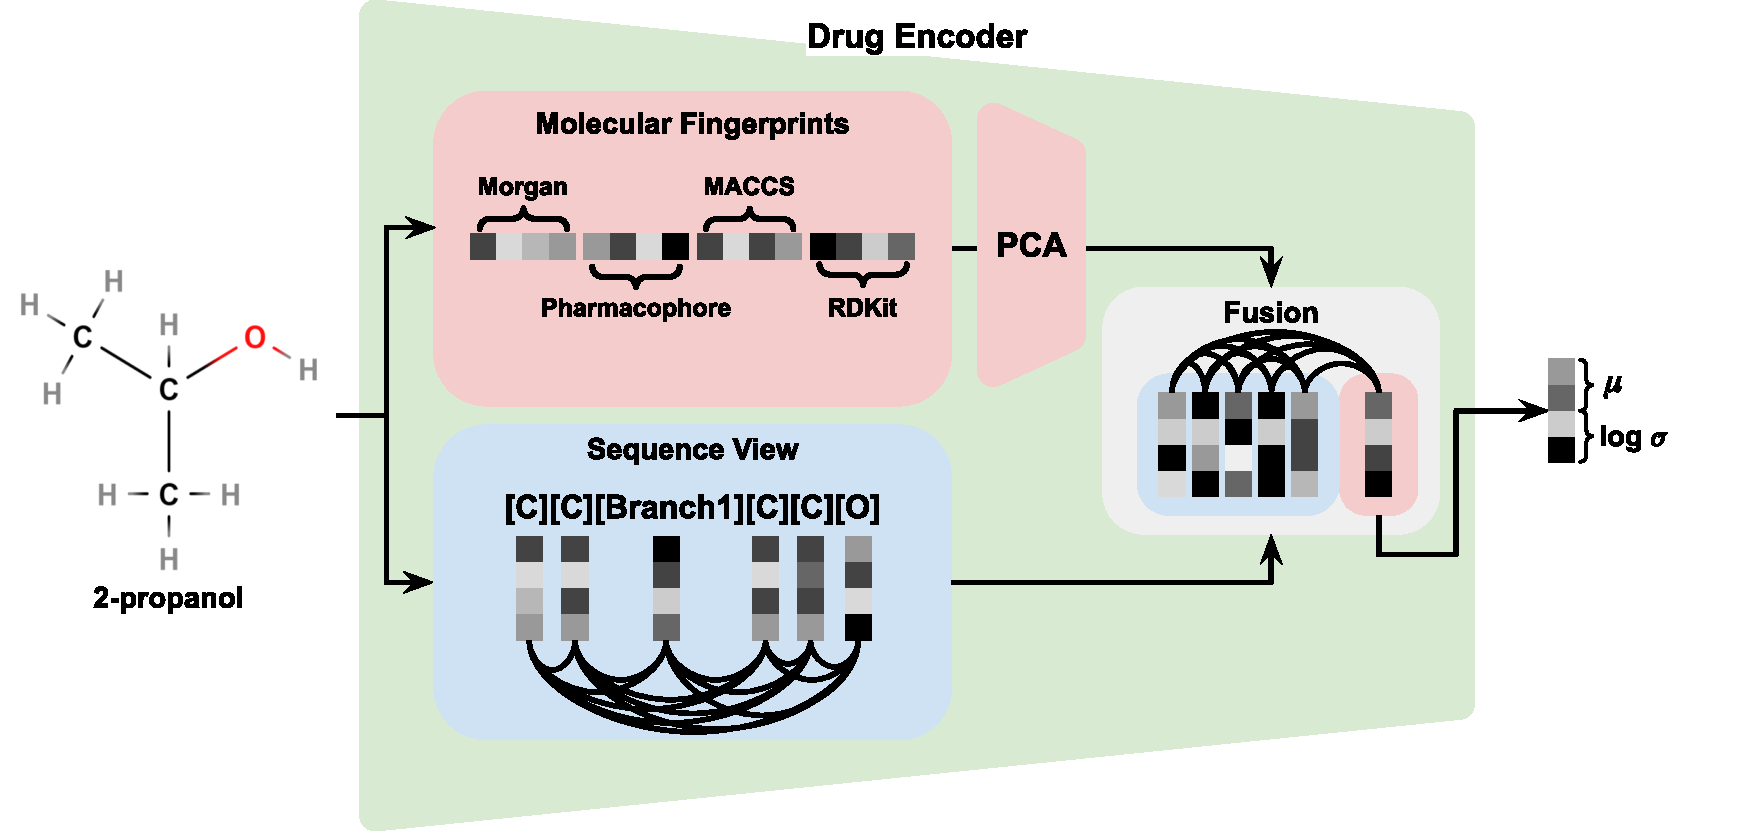
\includegraphics[width=\linewidth]{figs/model/drug_encoder.pdf}

    \caption[The drug encoder.]{The drug encoder. Fixed molecular fingerprints and token-level SELFIES representations are combined by a fusion Transformer. The state at the fingerprint position is projected into the parameters $\mu_d$ and $\log\sigma_d^2$ of the molecular posterior.}

    \label{fig:encoder}

\end{figure}

For a molecule $d$, the molecular encoder defines a diagonal Gaussian posterior
\begin{equation*}
    q_\phi(z\mid d)
    =
    \Ncal\!\left(
    \mu_d,
    \operatorname{diag}(\sigma_d^2)
    \right).
\end{equation*}

Here, $\mu_d$ gives the location of molecule $d$, and $\sigma_d^2$ gives its variance along each latent coordinate. The diagonal covariance allows the encoder to learn a separate spread in each direction.

\paragraph{Drug decoder.}

Figure \ref{fig:decoder} shows how a latent sample is converted back into a molecule. The decoder receives the latent representation $z$ together with the protein representation. The source of $z$ differs between training and generation, but its use by the decoder is the same.

The decoder is an autoregressive Transformer with causal self-attention. Each next token is predicted using the tokens already written: in the figure, the prefix \texttt{<BOS>[C][C]} is followed by \texttt{[Branch1]}. Subsequent predictions can therefore account for earlier choices because those choices become part of the input. Cross-attention additionally gives each decoder position access to two memory representations: a projection of $z$ and a projection of the conditioning protein embedding.

After each Transformer layer, a protein-dependent affine transformation further modifies the hidden states. It learns a scale and a shift from the protein representation, allowing the same decoder to adapt its intermediate representations to different proteins. These transformations are initialized as the identity, allowing reconstruction to develop before they acquire a conditioning effect through optimization.

Training uses teacher forcing: the decoder receives the true preceding tokens and minimizes next-token cross-entropy over non-padding positions. Generation begins with the beginning-of-sequence token and uses each sampled token as input to the next step. It stops when an end-of-sequence token is sampled or the maximum length of 128 tokens is reached. Padding, beginning-of-sequence, and unknown tokens cannot be sampled as molecular content, and termination is allowed only after at least one molecular token has been produced.

The final SelVAEGen configurations generate SELFIES. These strings are parsed and sanitized with RDKit before evaluation. Unless otherwise stated, the next-token sampling temperature is one. The temperature experiment in Section \ref{sec:temp} changes this sampling parameter while keeping the trained model fixed.

\begin{figure}[ht]

    \centering

    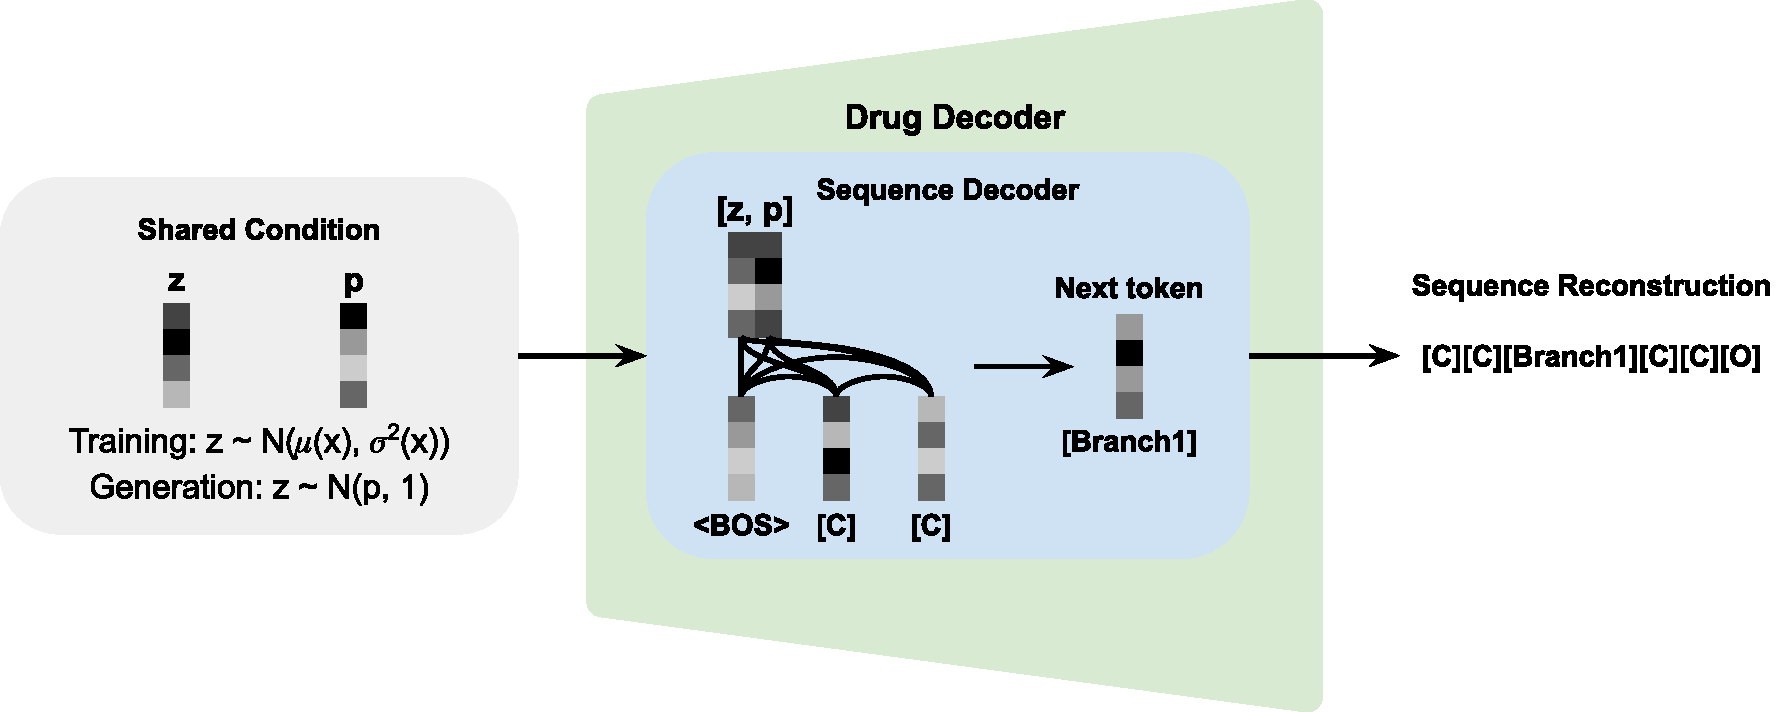
\includegraphics[width=\linewidth]{figs/model/drug_decoder.pdf}

    \caption[The drug decoder.]{The autoregressive drug decoder. The latent representation and protein representation are supplied through cross-attention, while protein-dependent affine transformations provide additional conditioning after each Transformer layer.}

    \label{fig:decoder}

\end{figure}

During training, a latent representation of the molecule is sampled using the reparameterization
\begin{equation*}
    z
    =
    \mu_d
    +
    \sigma_d\odot\epsilon,
    \qquad
    \epsilon\sim\Ncal(0,I).
\end{equation*}

The decoder receives this sample together with the protein representation, defining the conditional distribution
\begin{equation*}
    p_\theta(d\mid z,m_\psi(P)).
\end{equation*}

At generation time there is no input molecule. Instead, the latent representation is sampled directly from the protein-conditioned prior,
\begin{equation*}
    z
    \sim
    \Ncal\!\left(
    m_\psi(P),
    I
    \right),
\end{equation*}
and decoded conditionally on the requested protein. The same decoder must therefore work with samples from the molecular posterior during reconstruction and from the protein prior during generation. This is the reason for bringing those distributions together during training.

As in the VAE introduced in Chapter \ref{sec:literature}, reconstruction and prior regularization are combined in a variational lower bound:
\begin{equation*}
    \log p(d\mid P)
    \geq
    \E_{q_\phi(z\mid d)}
    \left[
        \log p_\theta(d\mid z,m_\psi(P))
        \right]
    -
    \KL\!\left(
    q_\phi(z\mid d)
    \,\|\,
    p_\psi(z\mid P)
    \right).
\end{equation*}

The first term rewards reconstructing the molecule from its posterior sample and the protein representation. The prior regularization loss brings that posterior towards the prior from which generation will later sample. To additionally teach the relative affinity relationships, we need a score describing how compatible a molecular representation is with a protein.

\paragraph{Target compatibility.}

A drug has high target compatibility when its latent mean lies in a region of high density under the protein-conditioned prior. Since that prior has fixed identity covariance, compatibility can be expressed through the distance between the molecular mean and the protein mean:
\begin{equation*}
    s(d,P)
    =
    -\frac{1}{2}
    \left\|
    \mu_d-m_\psi(P)
    \right\|_2^2.
\end{equation*}

The score is highest when $\mu_d$ and $m_\psi(P)$ coincide and decreases as they move apart. We assume that a latent space can be learned in which differences in this score follow experimentally observed affinity rankings. The score therefore supplies an ordering of interactions.

The proposed ranking and distributional losses use this compatibility score, which is calculated from the model's own representations and is distinct from the affinity estimates produced by the external oracles. Its connection to the protein prior follows directly from the Gaussian density. Since
\begin{equation*}
    p_\psi(z\mid P)
    =
    \Ncal\!\left(
    m_\psi(P),I
    \right),
\end{equation*}
evaluating its log density at the molecular latent mean gives
\begin{equation*}
    \log p_\psi(\mu_d\mid P)
    =
    -\frac{D}{2}\log(2\pi)
    -
    \frac{1}{2}
    \left\|
    \mu_d-m_\psi(P)
    \right\|_2^2
    =
    -\frac{D}{2}\log(2\pi)
    +
    s(d,P),
\end{equation*}
where $D=128$ is the dimensionality of the latent space. Therefore, for two molecules evaluated against the same protein,
\begin{equation*}
    \log p_\psi(\mu_{d_1}\mid P)
    -
    \log p_\psi(\mu_{d_2}\mid P)
    =
    s(d_1,P)
    -
    s(d_2,P),
\end{equation*}
because the Gaussian normalization constant cancels. A larger compatibility difference therefore corresponds exactly to a larger log-likelihood difference under the protein-conditioned latent distribution. Section \ref{sec:losses} uses this relation to train compatibility scores from measured affinity orderings.

\subsection{Training objectives}\label{sec:losses}
The complete objective contains five terms: the reconstruction loss $\mathcal{L}_{\mathrm{recon}}$, the prior regularization loss $\mathrm{KL}$, the affinity ranking loss $\mathcal{L}_{\mathrm{aff}}$, the selectivity ranking loss $\mathcal{L}_{\mathrm{sel}}$, and the distributional selectivity loss $\mathcal{L}_{\mathrm{dist}}$. Together, they teach the model how to reconstruct molecules, where to sample for a protein, and how to organize relative compatibilities. Equation \ref{eq:full_loss} groups the reconstruction loss, the prior regularization loss, and the three ranking and distributional losses. Figure \ref{fig:losses} illustrates the first four terms.

The purpose of the ranking and distributional losses can first be understood at the level of distributions. Chapter \ref{sec:metrics} evaluates whether affinities to intended targets tend to exceed affinities to off-target proteins. During training, the model works with the corresponding latent compatibility scores. For a molecule measured against several proteins, the desired arrangement places it in a region more compatible with its preferred protein than with the alternatives. Across molecules, these advantages should occur consistently, separating preferred-target from off-target compatibilities. This explains why the objectives concern differences and their spread: a uniform increase in compatibility would not establish a target preference. The resulting geometry is intended to support the separation of predicted affinity distributions examined in Chapter \ref{sec:results}, without requiring a uniform rise in absolute affinity.

All affinity information used to calculate the ranking and distributional losses comes from experimentally observed training pairs. The affinity oracles are used to evaluate generated molecules and do not provide gradients or affinity estimates for these losses. The training comparisons therefore depend on measured affinities, while generated molecules are later evaluated using the oracles discussed in Section \ref{sec:oracles}.

\begin{figure}[H]
    \centering
    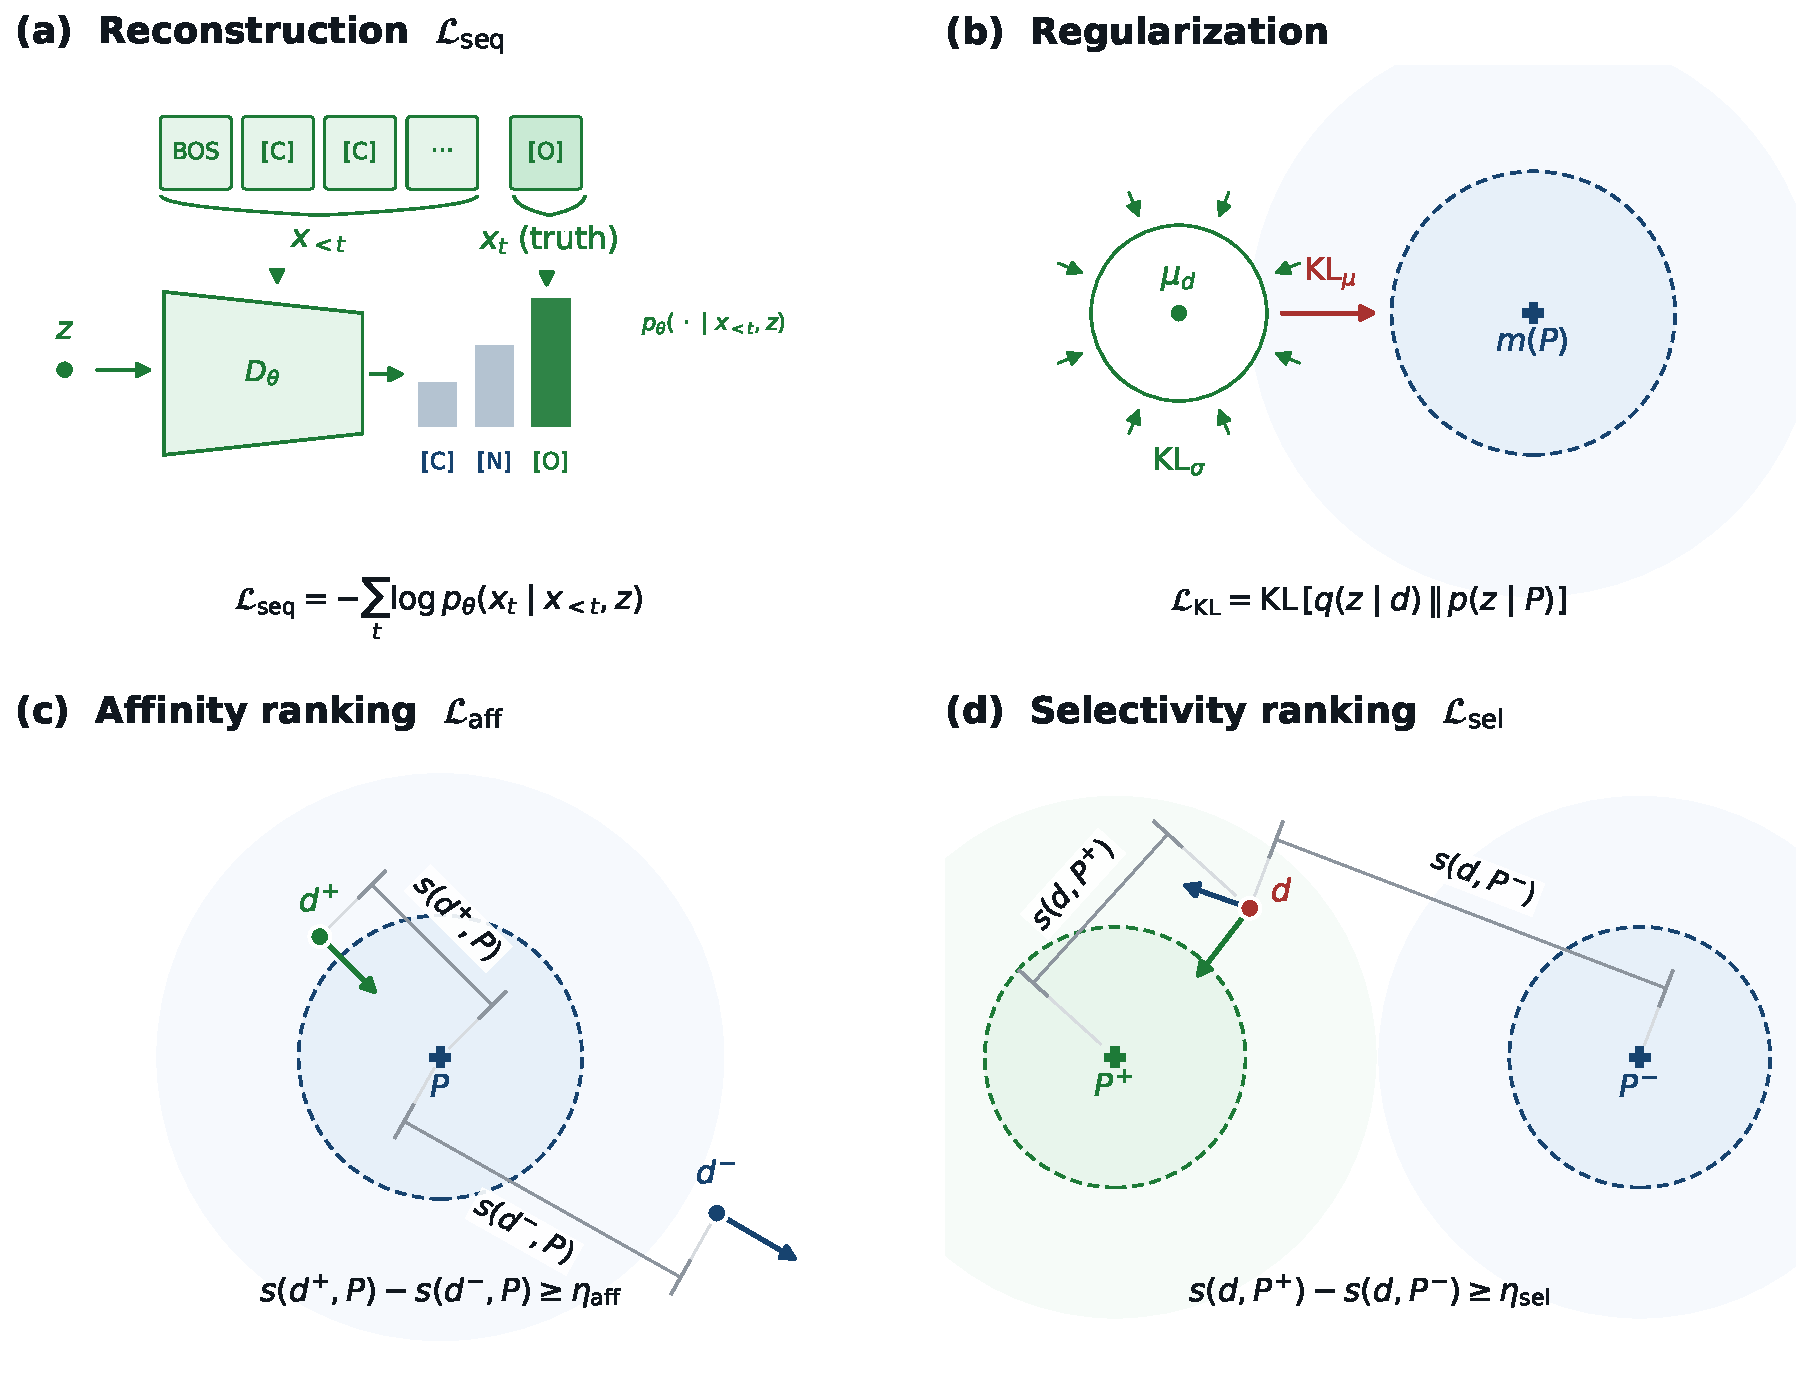
\includegraphics[width=\linewidth]{figs/model/losses.pdf}
    \caption[The training objectives, geometrically.]{How the losses organize the latent
        space. \textbf{(a)} The reconstruction loss requires the code to retain molecular information
        from which the decoder can recover the input string. \textbf{(b)} The prior regularization loss
        brings the molecular posterior mean $\mu_d$ towards the conditioning protein's
        Gaussian and its variance towards one, matching the distribution used for generation.
        \textbf{(c)} The affinity ranking loss compares two molecules for one protein and encourages
        the stronger measured binder to have higher compatibility by the margin
        $\eta_{\mathrm{aff}}$. \textbf{(d)} The selectivity ranking loss compares one molecule against
        two proteins and encourages higher compatibility with the protein it binds more
        strongly. In both ranking panels the dimension lines mark the latent spans that the
        compatibility score reads. Since $s(d,P)$ is minus half the squared distance between the
        molecular mean and the protein mean, a shorter span is a higher score, and each of these
        losses asks for one span to be shorter than the other by its margin.}
    \label{fig:losses}
\end{figure}

\paragraph{Reconstruction loss.}
Reconstruction teaches the decoder to recover an observed molecule from its latent representation. For the sequence decoder, this means predicting the next molecular token from the true preceding tokens. Let $\mathbf{x}=(x_1,\ldots,x_T)$ be the tokenized molecular string. Its reconstruction loss is
\begin{equation*}
    \mathcal{L}_{\mathrm{seq}}
    =
    -\sum_{t=1}^{T}
    \log
    p_{\theta}
    \left(
    x_t
    \mid
    x_{<t},z
    \right),
\end{equation*}
where $z$ is sampled from the molecular encoder's posterior and $x_{<t}$ denotes the tokens preceding position $t$. Each term penalizes assigning low probability to the observed next token.

\paragraph{Prior regularization loss.}
Reconstruction uses samples from molecular posteriors, but generation samples from protein priors. The prior regularization loss brings these distributions together by penalizing the KL divergence from the molecular posterior to the corresponding protein-conditioned Gaussian:

\begin{equation*}
    p(z\mid P)
    =
    \mathcal{N}
    \left(
    m_\psi(P),I
    \right),
\end{equation*}

Here, $m_\psi(P)$ denotes the protein prior mean defined above. The molecular encoder's approximate posterior is
\begin{equation*}
    q(z\mid d)
    =
    \mathcal{N}
    \left(
    \mu_d,
    \operatorname{diag}(\sigma_d^2)
    \right).
\end{equation*}

For this choice of posterior and prior, the prior regularization loss can be decomposed into contributions from the posterior mean and variance:
\begin{equation*}
    \mathrm{KL}
    =\underbrace{
        \frac{1}{2}
        \left\|
        \mu_d-m_\psi(P)
        \right\|_2^2}_{\mathrm{KL}_{\mu}}+\underbrace{\frac{1}{2}
        \sum_r
        \left(
        \sigma_{d,r}^2
        -
        1
        -
        \log\sigma_{d,r}^2
        \right)}_{
        \mathrm{KL}_{\sigma}}.
\end{equation*}

The mean component $\mathrm{KL}_{\mu}$ penalizes the distance between the molecular mean and the protein mean. The variance component $\mathrm{KL}_{\sigma}$ brings each posterior variance towards the prior variance of one, with $r$ indexing latent coordinates. These two contributions regulate where the molecular distribution lies and how widely it spreads.
\paragraph{Affinity ranking loss.}
The two ranking losses apply the same comparison along different axes of the affinity matrix. Affinity ranking holds a protein fixed and compares two molecules. Selectivity ranking holds a molecule fixed and compares two proteins. Panels (c) and (d) of Figure \ref{fig:losses} show this distinction. The first organizes molecules by affinity to a target, while the second directly teaches relative target preference.

For affinity ranking, consider two molecules with measured affinities to a protein $P$. Denote the stronger binder by $d^{+}$ and the weaker by $d^{-}$. Their compatibility scores are $s^+=s(d^{+},P)$ and $s^-=s(d^{-},P)$. We want $s^+$ to exceed $s^-$, meaning that the stronger binder lies in a region of greater likelihood under the protein's latent distribution, as established in Section \ref{sec:varmod}.

Let $A^+$ and $A^-$ be their measured affinities to $P$. The size of this experimental difference determines the comparison's weight:
\begin{equation*}
    w
    =
    \left|
    A^{+}-A^{-}
    \right|.
\end{equation*}

The affinity ranking loss is defined as the weighted margin loss
\begin{equation*}
    \mathcal{L}_{\mathrm{aff}}
    =
    \frac{
        \displaystyle
        \sum
        w\,
        \max
        \left(
        0,
        \eta_{\mathrm{aff}}
        -
        \left(
        s^{+}-s^{-}
        \right)
        \right)
    }{
        \displaystyle
        \sum w
    },
\end{equation*}

The sums run over all the possible molecular comparisons in the training batch, and $\eta_{\mathrm{aff}}$ is the required compatibility margin. When $s^+-s^-$ is smaller than this margin, the comparison incurs a penalty. Once the gap reaches the margin, its penalty is zero. Weighting by $w$ gives less influence to molecules whose measured affinities are only weakly distinguished.

\paragraph{Selectivity ranking loss.}
Selectivity ranking instead fixes one molecule $d$ and compares two proteins. Let $P^{+}$ be the protein for which its measured affinity is higher and $P^{-}$ the one for which it is lower. We want the molecular representation to have higher likelihood under the prior of $P^{+}$ than under that of $P^{-}$. Because both priors have identity covariance, their Gaussian normalization constants cancel in the log-likelihood difference. The desired ordering can therefore again be expressed through the compatibility scores
\begin{equation*}
    s^{+}=s(d,P^{+}),
    \qquad
    s^{-}=s(d,P^{-}),
\end{equation*}
and the pair is weighted by the corresponding observed affinity gap,
\begin{equation*}
    w
    =
    \left|
    A^{+}-A^{-}
    \right|.
\end{equation*}

The loss is
\begin{equation*}
    \mathcal{L}_{\mathrm{sel}}
    =
    \frac{
        \displaystyle
        \sum
        w\,
        \max
        \left(
        0,
        \eta_{\mathrm{sel}}
        -
        \left(
        s^{+}-s^{-}
        \right)
        \right)
    }{
        \displaystyle
        \sum w
    }.
\end{equation*}

Here, $\eta_{\mathrm{sel}}$ is the required compatibility margin, and the sums run over the protein comparisons. As with affinity ranking, a comparison contributes only while its compatibility gap is below the margin. The distinction is the object being compared: $\mathcal{L}_{\mathrm{aff}}$ ranks molecules for a fixed protein, whereas $\mathcal{L}_{\mathrm{sel}}$ ranks proteins for a fixed molecule. The latter therefore requires molecules with experimental measurements against multiple proteins.

Short videos illustrating the geometry of these losses are available in the ``docs/videos'' folder of the project \href{https://github.com/DutraIRS/SelVAEGen}{GitHub repository}. In particular, they illustrate the necessity of introducing the margins so as to avoid a trivial solution of push the lower affinity elements towards infinity.

\paragraph{Distributional selectivity loss.}
Pairwise ranking teaches individual orderings, but we also want the compatibility advantage to be positive and consistent across molecules. The distributional selectivity loss combines two requirements: each molecule should have a sufficient average advantage for its preferred protein, and the mean advantage across the batch should be large relative to its spread.

For a molecule $d$, let $P^{*}$ be the protein with its highest recorded affinity and $\mathcal{P}_{\mathrm{off}}$ the set of off-target proteins used in the comparison. Its mean compatibility gap is
\begin{equation*}
    \gamma(d)
    =
    \frac{1}{|\mathcal{P}_{\mathrm{off}}|}
    \sum_{P\in\mathcal{P}_{\mathrm{off}}}
    \left[
        s(d,P^{*})
        -
        s(d,P)
        \right].
\end{equation*}

A positive $\gamma(d)$ means that the molecule is more compatible with $P^{*}$ than with its off-target proteins on average. The directional loss requires this advantage to reach a margin $\eta_{\mu}$:
\begin{equation*}
    \mathcal{L}_{\mathrm{dir}}
    =
    \mathbb{E}_{d}
    \left[
        \max
        \left(
        0,
        \eta_{\mu}
        -
        \gamma(d)
        \right)
        \right].
\end{equation*}

This penalty is applied to individual molecules. The separation loss considers the batch as a whole, requiring the mean gap divided by its standard deviation to reach $\eta_e$:
\begin{equation*}
    \mathcal{L}_{\mathrm{sep}}
    =
    \max
    \left(
    0,
    \eta_e
    -
    \frac{
        \mathbb{E}[\gamma]
    }{
        \operatorname{sd}(\gamma)
    }
    \right).
\end{equation*}

The ratio $\mathbb{E}[\gamma]/\operatorname{sd}(\gamma)$ measures the size of the average advantage relative to its variation across molecules. For a given positive mean, a wider spread reduces this ratio. The term therefore discourages an advantage that is large on average but inconsistent from one molecule to the next. The complete distributional selectivity loss is
\begin{equation*}
    \mathcal{L}_{\mathrm{dist}}
    =
    (1-\lambda)
    \mathcal{L}_{\mathrm{sep}}
    +
    \lambda
    \mathcal{L}_{\mathrm{dir}},
\end{equation*}
where $\lambda\in[0,1]$ balances the directional loss for individual molecules and the separation loss for the batch.

The margins specify how much separation is sufficient. Without this stopping point, an objective that continually rewards a larger compatibility difference could be improved simply by moving non-preferred representations increasingly far away. The hinge form instead becomes zero once its required margin is met, so that comparison supplies no further gradient to enlarge the gap. It encourages the desired ordering without continuing to reward unbounded separation \parencite{Hadsell_Chopra_LeCun_2006}.

The final objective combines these five terms, with the coefficients $\beta$ controlling how much each contributes:
\begin{equation}
    \label{eq:full_loss}
    \mathcal{L}=\underbrace{
        \beta_{\mathrm{recon}}\mathcal{L}_{\mathrm{recon}}
    }_{\text{reconstruction}} +
    \underbrace{
        \beta_{\mathrm{KL}}\mathrm{KL}
    }_{\text{prior regularization}} +
    \underbrace{
        \beta_a\mathcal{L}_{\mathrm{aff}}
        +
        \beta_s\mathcal{L}_{\mathrm{sel}}
        +
        \beta_d\mathcal{L}_{\mathrm{dist}}
    }_{\text{ranking and distributional losses}}.
\end{equation}

Optimization uses AdamW \parencite{Loshchilov_Hutter_2019}, which applies weight decay separately from the gradient-based parameter update. Hyperparameters, including loss weights and margins, are selected with Optuna \parencite{Akiba_Sano_Yanase_Ohta_Koyama_2019} using the Tree-structured Parzen Estimator (TPE) procedure \parencite{Bergstra_Bardenet_Bengio_Kegl_2011}. Each trial trains a model with the proposed configuration and generates molecules for proteins in the validation split. The configuration is scored by Effective $\Delta$, with higher values preferred. This selection criterion rewards selective output while accounting for the validity, uniqueness, novelty, and on-target affinity requirements defined in Chapter \ref{sec:metrics}.

\chapteropening
{Results}
{figs/chapters/results.pdf}
{0.85\textwidth}
{Predicted on-target and ranked off-target affinities on KIBA. For each of the 23 test proteins, each model generates 256 molecules. Colored bars show the mean predicted affinity to the conditioning protein. Gray bars show the mean predicted affinity to off-target proteins after ranking them by affinity, so that the first gray bar corresponds to the strongest predicted off-target, the second to the second strongest, and so on. The dashed line indicates the dataset’s positive-affinity threshold. The $\Delta$ score is defined as the height of the colored bar minus the mean height of the gray bars. Among the models compared, SelVAEGen is the only one that shows both a positive $\Delta$ score and a mean on-target affinity above the dataset’s threshold.}
{%
    \lettrine[
        lines=2,
        lhang=0.0,
        loversize=0.0
    ]{A}{}\textit{t this stage, the model can be evaluated with the metrics of Chapter \ref{sec:metrics}, in comparison with three recent protein-targeted generators. The question is whether the molecules they produce preferentially bind to the protein for which they were generated. We first describe the data and the affinity predictors used to assess those molecules. We then compare generation quality, predicted affinity and selectivity, before examining individual examples and the effects of the model's main design choices. Figure \ref{fig:results_first} shows that comparison on one of the datasets, KIBA.}
}[Parla! [Speak!]][Michelangelo][sec:results][Predicted on-target and ranked off-target affinities on the KIBA dataset.][fig:results_first]

\subsection{Datasets}\label{sec:datasets}

Four drug-target affinity datasets commonly used in the literature are considered here. They differ in the number of molecules and proteins they contain, the proportion of drug-protein pairs with a measured affinity, and the diversity of their targets. In order to ensure the quality and consistency of the datasets, we applied a series of curation steps to each one. The same curation criteria were applied to each dataset. We excluded:
\begin{itemize}
    \item Proteins with fewer than 50 or more than 2000 amino acids.
    \item Drugs whose SMILES string is longer than 128 characters.
    \item Proteins with fewer than 5 observed affinity values.
\end{itemize}

\paragraph{KIBA {\normalfont\parencite{Tang2014KIBA}}} contains affinity measurements for kinase inhibitors. Instead of reporting a single assay type, it combines $K_i$, $K_d$ and $\mathrm{IC}_{50}$ measurements from several sources into a common KIBA score. The threshold for a positive interaction is $12.1$ on this scale. Figure \ref{fig:kiba_data} shows the distributions of affinity values, protein and molecular string lengths, and the number of measurements per protein.

\begin{figure}[H]
    \centering
    
\includegraphics[width=0.8\textwidth]{figs/e0/kiba/distributions.pdf}
    \caption[Profile of the KIBA dataset.]{Profile of the KIBA dataset. \textbf{(a)} Distribution of recorded affinity values, with the dataset's positive-affinity threshold marked in red. \textbf{(b)} Distribution of protein lengths, measured as the number of amino acids in each unique protein. \textbf{(c)} Distribution of molecular string lengths for unique drugs. The red lines in \textbf{(b)} and \textbf{(c)} mark the filtering criteria. \textbf{(d)} Number of recorded affinity measurements per protein.}
    \label{fig:kiba_data}
\end{figure}

\paragraph{Davis {\normalfont\parencite{Davis2011}}} contains a complete panel of inhibitor-kinase measurements obtained under a single assay protocol. Every inhibitor was tested against every kinase, so the matrix of dissociation constants is fully observed. This provides direct comparisons between proteins for each molecule, although the collection of molecules is small. Figure \ref{fig:davis_data} shows its main characteristics.

\begin{figure}[H]
    \centering
    
\includegraphics[width=0.7\textwidth]{figs/e0/davis/distributions.pdf}
    \caption[Profile of the Davis dataset.]{Profile of the Davis dataset. \textbf{(a)} Distribution of recorded affinity values, with the dataset's positive-affinity threshold marked in red. \textbf{(b)} Distribution of protein lengths, measured as the number of amino acids in each unique protein. \textbf{(c)} Distribution of molecular string lengths for unique drugs. The red lines in \textbf{(b)} and \textbf{(c)} mark the filtering criteria. \textbf{(d)} Number of recorded affinity measurements per protein.}
    \label{fig:davis_data}
\end{figure}

\paragraph{BindingDB {\normalfont\parencite{Liu2007BindingDB}}} collects experimentally measured affinities from the literature, covering many assay types and targets. It contains a more diverse collection of examples, but measurements are available for only roughly two in every thousand drug-protein pairs. Figure \ref{fig:bindingdb_data} summarizes the dataset.

\begin{figure}[H]
    \centering
    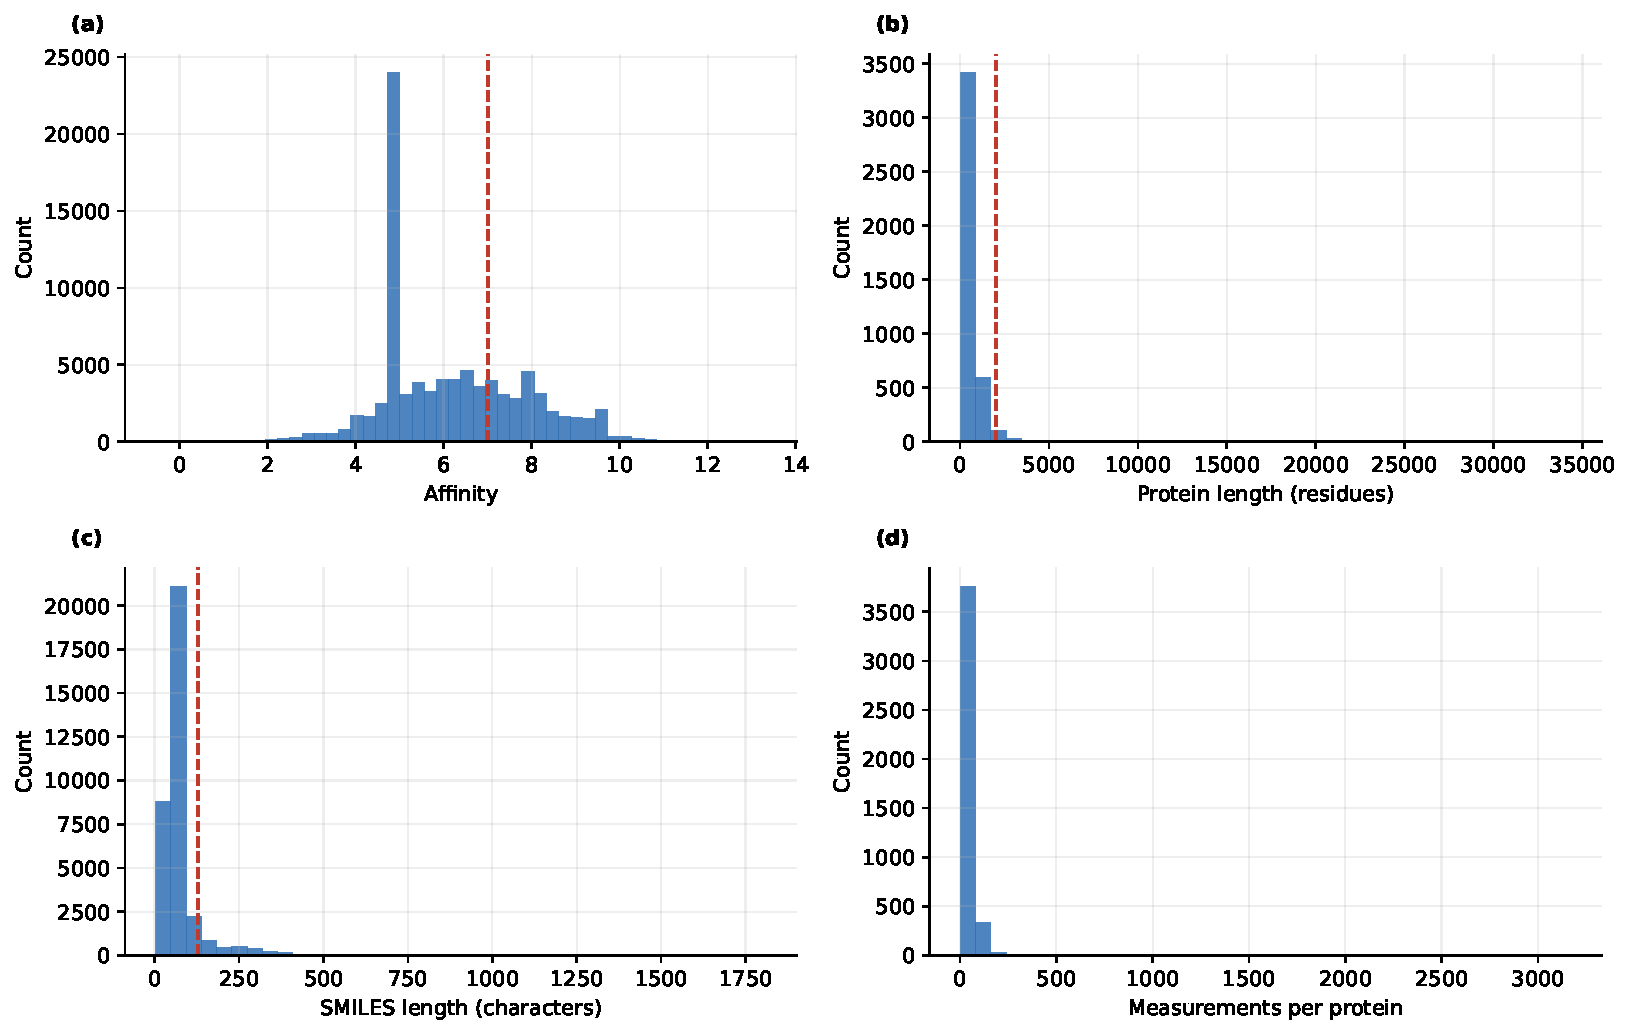
\includegraphics[width=0.7\textwidth]{figs/e0/bindingdb/distributions.pdf}
    \caption[Profile of the BindingDB dataset.]{Profile of the BindingDB dataset. \textbf{(a)} Distribution of recorded affinity values, with the dataset's positive-affinity threshold marked in red. \textbf{(b)} Distribution of protein lengths, measured as the number of amino acids in each unique protein. \textbf{(c)} Distribution of molecular string lengths for unique drugs. The red lines in \textbf{(b)} and \textbf{(c)} mark the filtering criteria. \textbf{(d)} Number of recorded affinity measurements per protein.}
    \label{fig:bindingdb_data}
\end{figure}

\paragraph{Papyrus {\normalfont\parencite{Bequignon2023Papyrus}}} is a large collection of bioactivity data with standardized molecular structures and quality filters. In this work, only high-quality entries for human proteins were retained. Figure \ref{fig:papyrus_data} shows its affinity distribution, the sizes of its molecules and proteins, and its coverage per protein.

\begin{figure}[h]
    \centering
    
\includegraphics[width=0.8\textwidth]{figs/e0/papyrus/distributions.pdf}
    \caption[Profile of the Papyrus dataset.]{Profile of the Papyrus dataset. \textbf{(a)} Distribution of recorded affinity values, with the dataset's positive-affinity threshold marked in red. \textbf{(b)} Distribution of protein lengths, measured as the number of amino acids in each unique protein. \textbf{(c)} Distribution of molecular string lengths for unique drugs. The red lines in \textbf{(b)} and \textbf{(c)} mark the filtering criteria. \textbf{(d)} Number of recorded affinity measurements per protein.}
    \label{fig:papyrus_data}
\end{figure}

The filters retained $98.44\%$, $92.81\%$, $89.03\%$, and $99.06\%$ of the observed affinities in KIBA, Davis, BindingDB and Papyrus, respectively. Table \ref{tab:datasets} reports the resulting collections. KIBA and Davis provide comparatively dense measurements, while BindingDB and Papyrus contain many more molecules but observe only a small fraction of their possible interactions. A large number of affinity records does not imply a large number of examples from which to learn selectivity.

\begin{table}[H]
    \centering
    \caption[Dataset statistics after filtering.]{Dataset statistics after the curation
        criteria above have been applied. \textbf{Drugs} and \textbf{Proteins} count the distinct
        molecules and distinct proteins that survive filtering. \textbf{Records} is the number of observed drug-protein affinities.
        \textbf{Density} expresses those records as a percentage of the
        $\text{Drugs}\times\text{Proteins}$ pairs that could in principle have been measured, so
        $100\%$ means every drug was tested against every protein and a small value means most of
        the matrix is unobserved. \textbf{Threshold} is the value on that dataset's own affinity
        scale at or above which a pair is treated as binding, which differs because KIBA reports a
        composite KIBA score while the other three report affinities on the $pKd$ scale.
        \textbf{Positive} is the percentage of records reaching that threshold.}
    \label{tab:datasets}
    \begin{tabular}{lrrrrrr}
        \toprule
        \textbf{Dataset} & \textbf{Drugs} & \textbf{Proteins} & \textbf{Records} & \textbf{Density (\%)} & \textbf{Threshold}& \textbf{Positive (\%)} \\
        \midrule
        KIBA & 2,015 & 225 & 115,822 & 25.55 & 12.10 & 20.86 \\
        Davis & 64 & 427 & 27,328 & 100.00 & 7.00 & 8.03 \\
        BindingDB & 31,053 & 1,200 & 77,412 & 0.21 & 7.00 & 30.43 \\
        Papyrus & 81,147 & 749 & 239,226 & 0.39 & 7.00 & 32.15 \\
        \bottomrule
    \end{tabular}
\end{table}

\subsubsection{Selectivity in the datasets}
Before training a selective generator, we need to consider what selectivity information is available in these datasets. Whether the observed data captures any selectivity at all, and how many good examples there are, are thus key questions to address before any training can begin.

For the first question, we retain drugs measured against at least three proteins and calculate an empirical $\Delta$ score from their observed affinities. Figure \ref{fig:e0_sel} shows the 20 highest-scoring drugs in each dataset. The on-target protein is taken to be the one with the highest measured affinity, and its score compares that affinity with the mean of its other measured affinities.

\begin{figure}[H]
    \centering
    \begin{subfigure}{0.49\linewidth}
        \centering
        
\includegraphics[width=\linewidth]{figs/e0/kiba/selectivity.pdf}
        \caption{KIBA}\label{fig:e0_sel_kiba}
    \end{subfigure}
    \hfill
    \begin{subfigure}{0.49\linewidth}
        \centering
        
\includegraphics[width=\linewidth]{figs/e0/davis/selectivity.pdf}
        \caption{Davis}\label{fig:e0_sel_davis}
    \end{subfigure}

    \begin{subfigure}{0.49\linewidth}
        \centering
        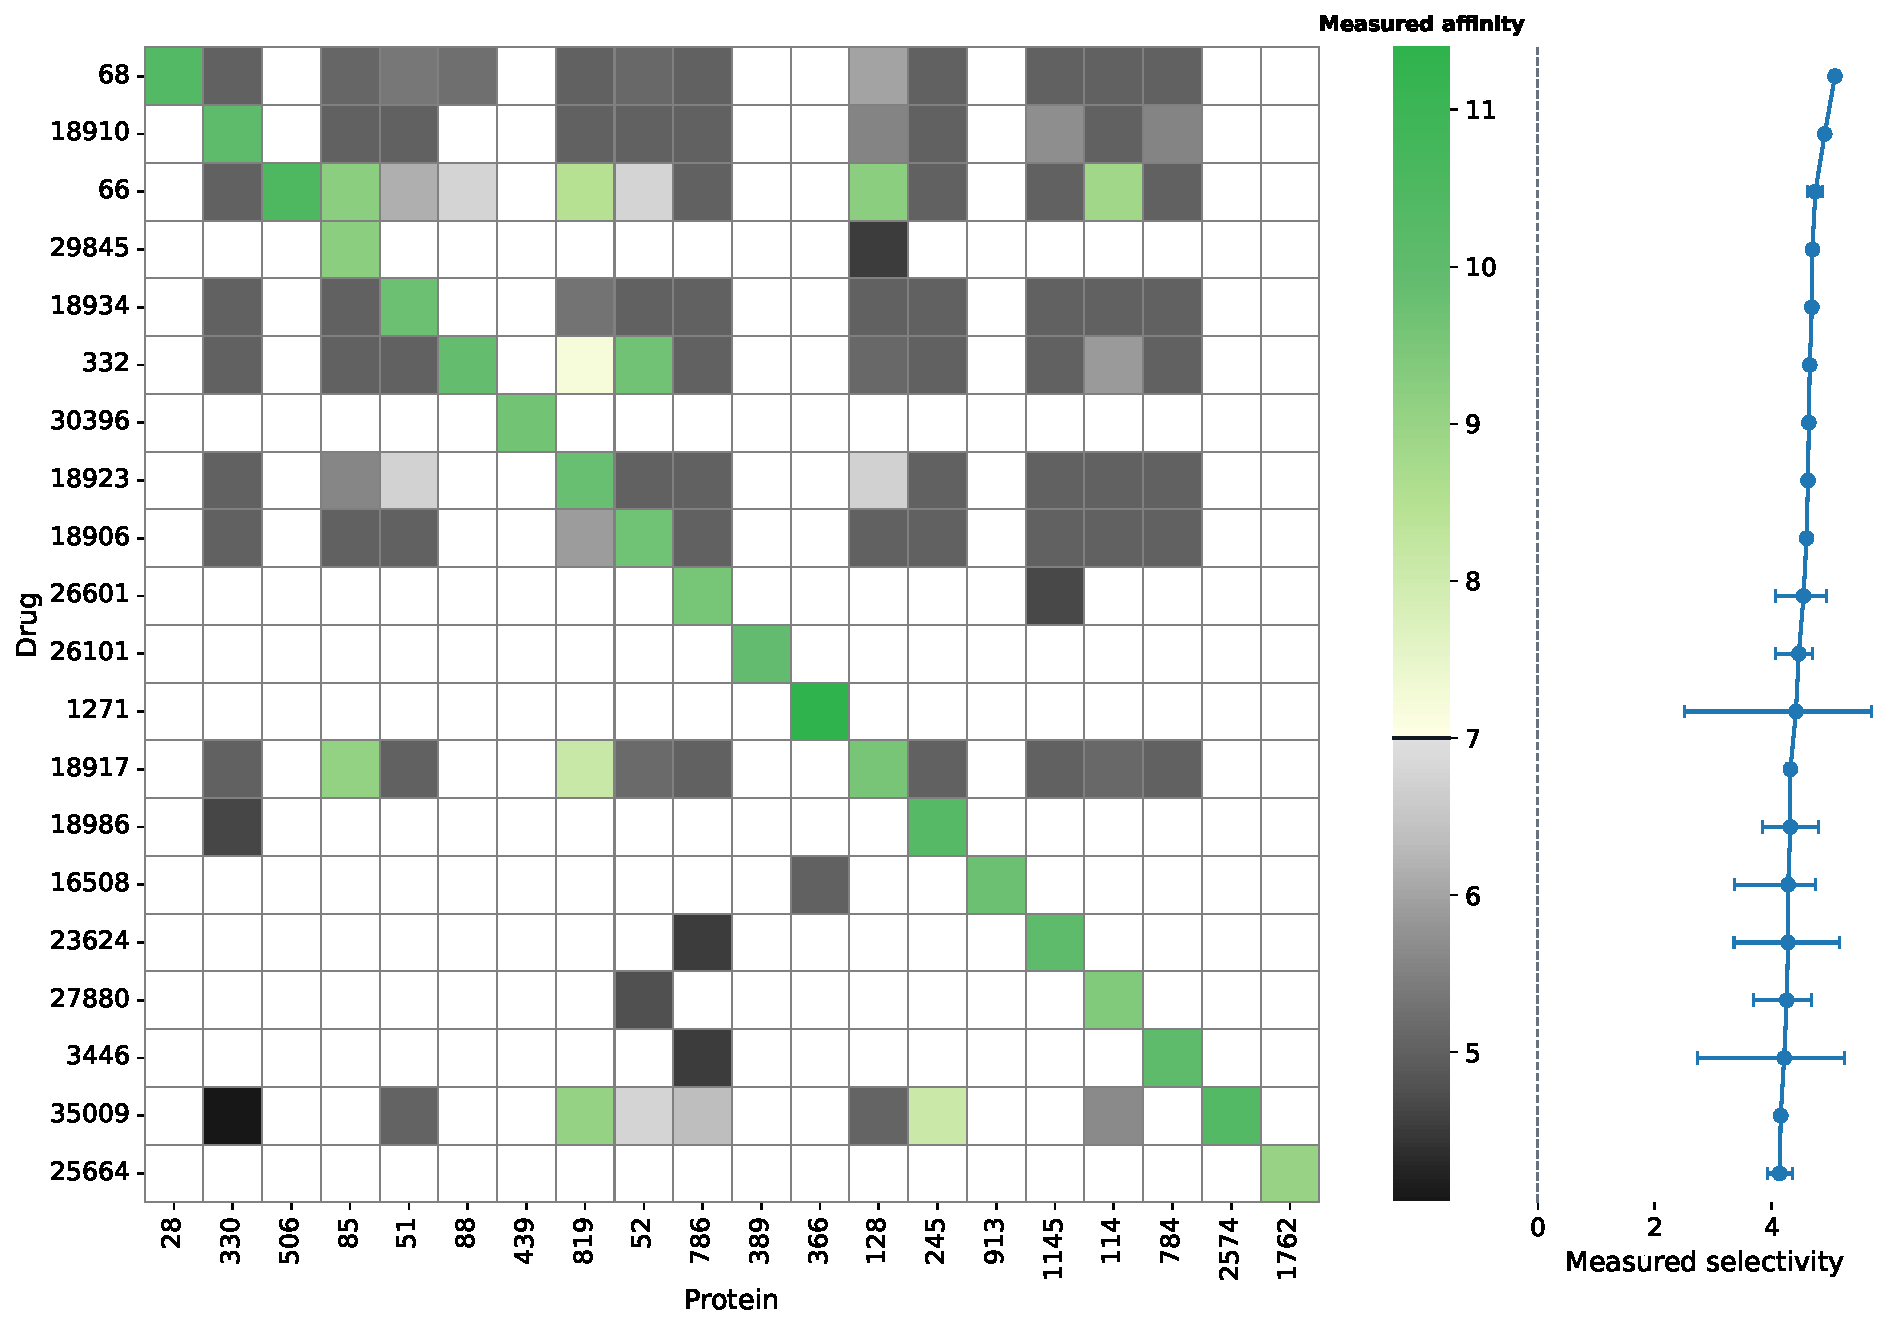
\includegraphics[width=\linewidth]{figs/e0/bindingdb/selectivity.pdf}
        \caption{BindingDB}\label{fig:e0_sel_bindingdb}
    \end{subfigure}
    \hfill
    \begin{subfigure}{0.49\linewidth}
        \centering
        
\includegraphics[width=\linewidth]{figs/e0/papyrus/selectivity.pdf}
        \caption{Papyrus}\label{fig:e0_sel_papyrus}
    \end{subfigure}
    \caption[Best selectivity examples in each dataset.]{The twenty drugs with the highest empirical $\Delta$ score among those measured against at least three proteins in \textbf{(a)} KIBA, \textbf{(b)} Davis, \textbf{(c)} BindingDB and \textbf{(d)} Papyrus. Each row is one drug, and the columns are the proteins preferred by these drugs, arranged so that each diagonal entry is the drug's best measured target. Cell color represents measured affinity. Blank cells indicate unmeasured pairs. Grayscale cells indicate affinity values below the dataset's threshold, and cells in green scale indicate higher affinity values. The strip on the right follows the same row order and gives each drug's empirical $\Delta$: its affinity for the best target minus its mean measured affinity for the remaining proteins, with a bootstrap interval over the off-target set. These examples use experimental data directly, without an oracle or generator. Their apparent selectivity depends on which proteins were measured, so they demonstrate the presence of selective examples within the observed data.}
    \label{fig:e0_sel}
\end{figure}

These examples show that the datasets contain molecules with a substantial preference among the proteins against which they were tested. They do not establish how common such examples are. Their apparent selectivity also depends on the choice of measured proteins: an unmeasured interaction could change the comparison. The figure therefore describes the strongest selectivity examples available in the data, within the limits of the observed panels.

The second question concerns the amount of training information. The selectivity ranking loss of Section \ref{sec:losses} compares two proteins for the same molecule. A drug measured against only one protein cannot supply this comparison, whereas a drug measured against $n$ proteins supplies $\binom{n}{2}$ pairs. Table \ref{tab:selectivity_supply} counts these pairs and shows how they are distributed over the molecules in each dataset.

\begin{table}[H]
    \centering
    \caption[Selectivity examples available in each dataset.]{How much
        selectivity information each dataset holds. A comparison is a pair of proteins
        measured against one common drug, which is the unit the selectivity ranking loss of
        Section \ref{sec:losses} consumes. A drug measured against $n$ proteins supplies
        $\binom{n}{2}$ of them, and a drug measured against one supplies none.
        \textbf{Drugs} is the number of distinct molecules. \textbf{Per drug} is the mean number
        of affinity records per drug. \textbf{$\geq 2$ targets} is the percentage of drugs
        measured against at least two distinct proteins, which is the percentage contributing any
        comparison at all. The remainder of each dataset contributes none.
        \textbf{Comparisons} is $\sum_d \binom{n_d}{2}$ over every drug $d$, the total the
        dataset supplies, and \textbf{Top 1\%} is the share of that total coming from the $1\%$ of
        drugs measured against the most proteins. A dataset may report a large total while almost
        all of it rests on a handful of heavily profiled compounds. All counts are taken over the
        same filtered collections as Table \ref{tab:datasets}.}
    \label{tab:selectivity_supply}
    \begin{tabular}{lrrrrr}
        \toprule
        \textbf{Dataset} & \textbf{Drugs} & \textbf{Per drug} &
        \textbf{$\geq 2$ targets} & \textbf{Comparisons} & \textbf{Top 1\%} \\
        \midrule
        KIBA      &  2,015 &  57.5 & 100.0\% & 5,653,431 &  4.3\% \\
        Davis     &     64 & 427.0 & 100.0\% & 5,820,864 &  1.6\% \\
        BindingDB & 31,053 &   2.5 &  23.9\% & 5,617,163 & 99.6\% \\
        Papyrus   & 81,147 &   2.9 &  40.5\% & 5,422,313 & 93.7\% \\
        \bottomrule
    \end{tabular}
\end{table}

The four datasets contain similar totals, between $5.4$ and $5.8$ million comparisons. What differs is how many molecules contribute to them. In KIBA and Davis, every drug has been measured against several proteins, and the median drug supplies $528$ and $90{,}951$ comparisons, respectively. In BindingDB and Papyrus, the most extensively measured $1\%$ of drugs accounts for $99.6\%$ and $93.7\%$ of all comparisons, and the median drug in either dataset supplies none at all. $76.1\%$ of BindingDB's drugs and $59.5\%$ of Papyrus's drugs have been measured against a single protein, and they contribute no comparison for the loss terms. In summary, although the total number of comparisons is similar, the distribution across molecules is very different.

Figure \ref{fig:e0_aff} makes this difference visible. Each row corresponds to a dataset. The left column groups measurements by drug, so it shows how many proteins can be compared for a given molecule. The right column groups the same measurements by protein, showing how many molecules can be compared for a given target.
In principle, it appears that all datasets have good examples in both cases, with sufficient vertical spread for each measurement. On closer inspection, however, the asymmetry in coverage becomes apparent, particularly in BindingDB and Papyrus, where many drugs have very few measurements compared to the number of proteins.
The Figure \ref{fig:e0_thin} reduces the display to fifty evenly spaced groups on each axis so that individual measurements are easier to distinguish.
KIBA has substantial coverage in both directions, with $56.9$ measurements per drug and $513.8$ per protein. Davis is the complete case, with each of its $64$ drugs measured against every protein. Papyrus is strongly asymmetric: it has $226.1$ measurements per protein but only $2.9$ per drug. Its protein panels therefore contain dense columns, while individual drugs often have only two or three measurements. BindingDB is sparse in both directions, with $2.5$ measurements per drug and $20.9$ per protein. For the selectivity ranking loss, the relevant coverage is on the left.

\begin{figure}[H]
    \centering
    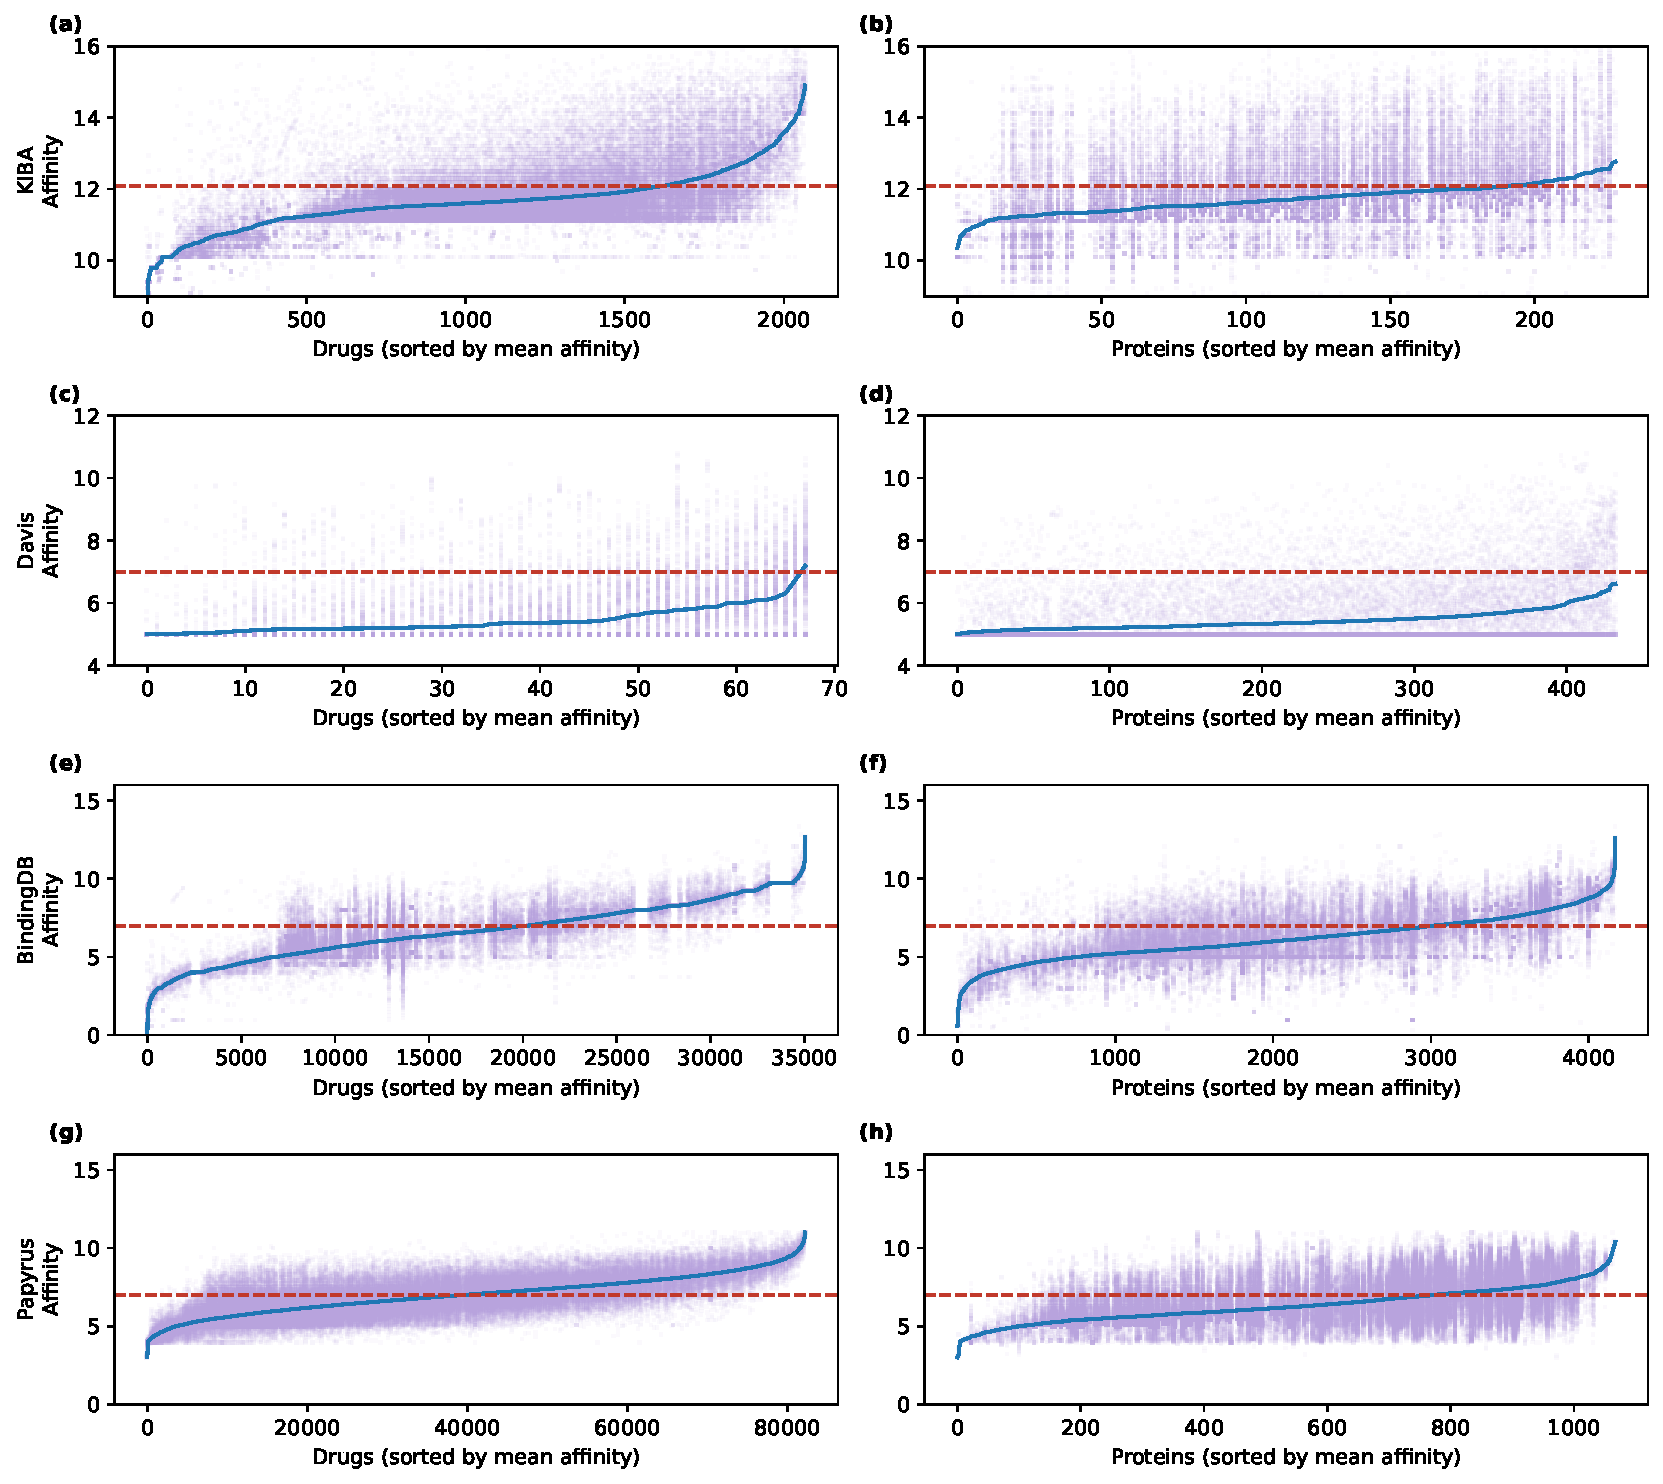
\includegraphics[width=\textwidth]{figs/e0/affinity_full.pdf}
    \caption[Measured affinity per drug and per protein, all four datasets.]{Recorded affinities grouped by drug in the left column and by protein in the right. Rows correspond to \textbf{(a, b)} KIBA, \textbf{(c, d)} Davis, \textbf{(e, f)} BindingDB and \textbf{(g, h)} Papyrus. Each purple square is one measurement, the blue line is the group mean, and the red dashed line is the dataset's positive-affinity threshold. Groups are ordered horizontally by mean affinity. The two panels in each row share a vertical scale. The left column shows the measurements available for comparing proteins for a fixed drug, as required by the selectivity ranking loss. The two largest datasets concentrate more measurements per protein than per drug.}
    \label{fig:e0_aff}
\end{figure}

\begin{figure}[H]
    \centering
    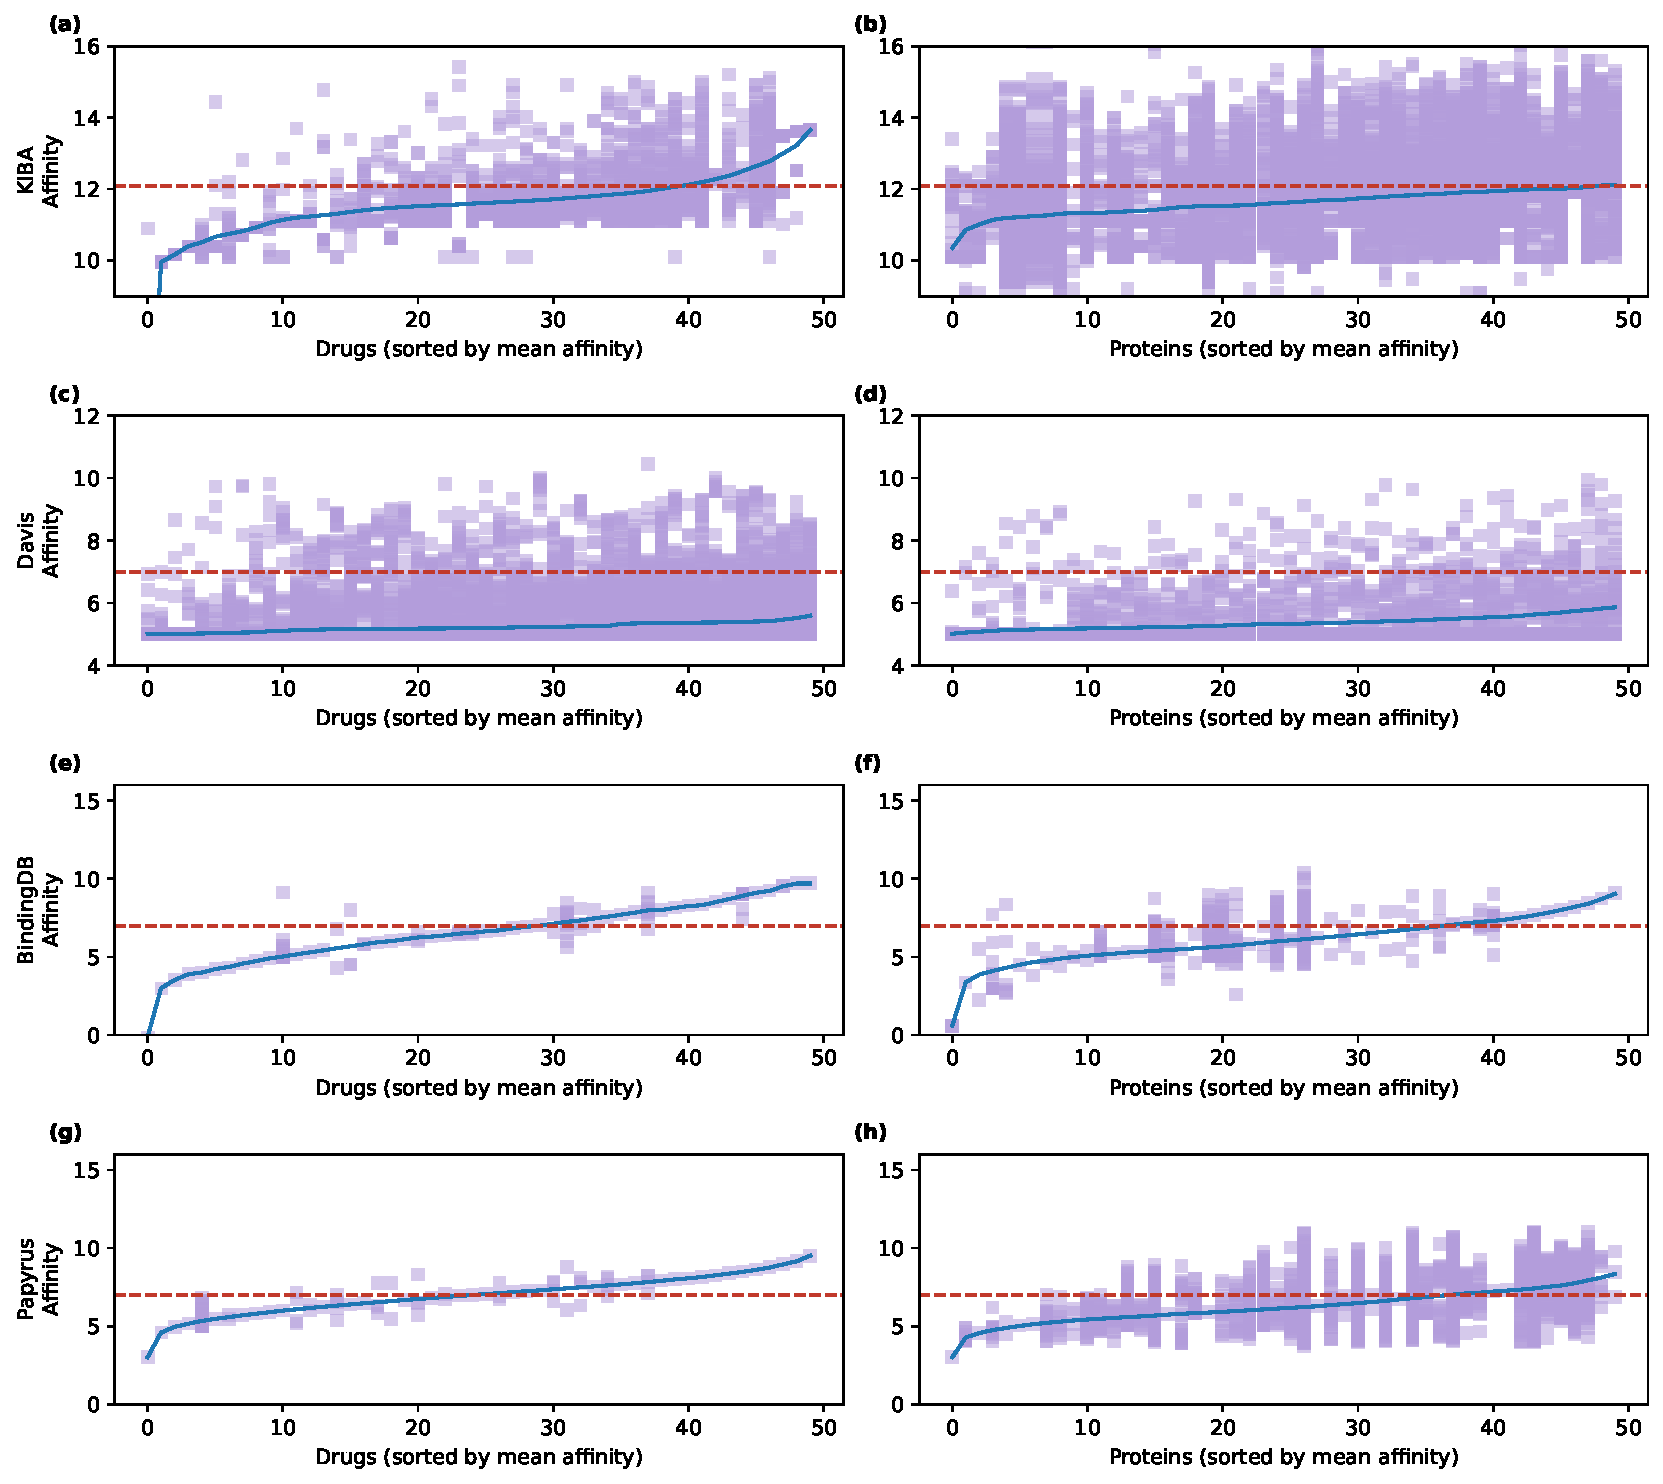
\includegraphics[width=\textwidth]{figs/e0/affinity_thinned.pdf}
    \caption[Measured affinity for fifty drugs and fifty proteins, all four datasets.]{The affinity groups of Figure \ref{fig:e0_aff}, reduced to fifty evenly spaced drugs in the left column and fifty evenly spaced proteins in the right. Rows correspond to \textbf{(a, b)} KIBA, \textbf{(c, d)} Davis, \textbf{(e, f)} BindingDB and \textbf{(g, h)} Papyrus. Groups are selected at a fixed stride through the ordering by mean affinity. Each purple square is one measurement: dense columns indicate groups with many observations, while columns with two or three squares indicate limited coverage. For the drug groups on the left, this coverage determines how many protein preferences can be compared. Davis retains its complete drug panel because it contains only $64$ drugs. BindingDB's and Papyrus's sparsity is evident in the thin columns.}
    \label{fig:e0_thin}
\end{figure}

The recorded values also include censoring floors. In Davis, $70.1\%$ of the affinities are exactly $5.00$, the value assigned when binding is not detected at the highest concentration tested. In BindingDB, $25.5\%$ of records take the same value.

These characteristics help explain why dataset size alone is an incomplete description of the training signal. Papyrus contains roughly twice as many affinity records as KIBA, spread over forty times as many drugs, yet supplies far fewer comparisons per drug. The denser datasets, Davis and KIBA, are also those on which the larger selectivity effects appear in Section \ref{sec:main}.

\subsubsection{Data split}
The oracles are trained separately on each dataset, using the hyperparameters reported in their original papers. Those of the baseline oracle were chosen arbitrarily. Their performance is evaluated on held-out affinity records and reported in Section \ref{sec:oracles}. Generator training uses measured affinities and does not use oracle predictions.

For the generators, we use an 80:10:10 split over proteins. Each protein, together with all affinity records involving it, is assigned to the training, validation or test set with probabilities 0.8, 0.1 and 0.1. A test protein is therefore unseen by the generator during training. Architecture and hyperparameter choices are made on the KIBA validation set, and the final comparisons use the test set of each dataset. All results are replicated five times with different data splits and random parameter initializations. For evaluation, each model produces 256 candidate drugs for each test protein.

\subsection{Oracles can partially capture selectivity}\label{sec:oracles}
The affinities of generated molecules are not experimentally measured in this work. They are estimated by the oracles introduced in Chapter \ref{sec:methods}, whose performance therefore determines how the generation results should be interpreted.

We examine two aspects of that performance. First, an oracle should recover the relative affinities of a molecule for different proteins, since measuring selectivity depends on being able to correctly estimate this comparison. Second, its predictions should remain informative for molecules that differ from the training examples. We assess the first aspect on the measured drug-protein pairs held out from each oracle's own training, which are real measurements and so allow a predicted ordering to be checked against an observed one. The second aspect doesn't have any reference, since a generated molecule may have never been measured. We examine it through the disagreement between the three oracles and its relation to similarity with the training molecules.

Table \ref{tab:oracle} reports affinity prediction performance. The oracles correctly recover the ordering of affinities in approximately $75\%$ of the directional comparisons. They capture part of the selectivity signal while still making a substantial number of ordering errors. The mean Directional Consistency across oracles is highest on Davis ($80.80\%$) and lowest on BindingDB ($76.27\%$), in agreement with the difference in their measurement density discussed above.

\begin{table}[ht]
    \centering
    \caption[Oracle performance on held-out affinity measurements.]{Oracle performance on each dataset's test set of measured drug-protein pairs. RMSE measures prediction error, CI measures agreement with observed affinity rankings, and Directional Consistency measures how often the oracle correctly orders the affinities of two proteins for a fixed drug. Lower RMSE and higher values of the two ranking metrics are desirable.}
    \label{tab:oracle}
    \begin{tabular}{llccc}
        \toprule
        \textbf{Dataset} & \textbf{Oracle} & \textbf{RMSE} & \textbf{CI} & \textbf{Dir. consistency} \\
        \midrule
        KIBA & Baseline & 0.4544 & 0.8193 & 0.7658 \\
        KIBA & GraphDTA & 0.5080 & 0.8169 & 0.7514 \\
        KIBA & GSDTA & 0.4478 & 0.8432 & 0.7927 \\
        \midrule
        Davis & Baseline & 0.5150 & 0.8672 & 0.8322 \\
        Davis & GraphDTA & 0.5556 & 0.8645 & 0.7947 \\
        Davis & GSDTA & 0.5520 & 0.8612 & 0.7972 \\
        \midrule
        BindingDB & Baseline & 0.7585 & 0.8692 & 0.7639 \\
        BindingDB & GraphDTA & 0.7613 & 0.8675 & 0.7557 \\
        BindingDB & GSDTA & 0.7448 & 0.8756 & 0.7686 \\
        \midrule
        Papyrus & Baseline & 0.6532 & 0.8374 & 0.7439 \\
        Papyrus & GraphDTA & 0.6361 & 0.8493 & 0.7829 \\
        Papyrus & GSDTA & 0.5925 & 0.8646 & 0.8280 \\
        \bottomrule
    \end{tabular}
\end{table}

We also examine whether predictions behave differently near the extremes of the affinity range. Figure \ref{fig:three_figures} compares the predicted and observed affinity quantiles on KIBA. The reported pattern does not show a pronounced deterioration at either end of the range. This complements the aggregate scores by showing how the predicted values are distributed across the observed scale.

\begin{figure}[H]
    \centering
    \begin{subfigure}{0.32\textwidth}
        \centering
        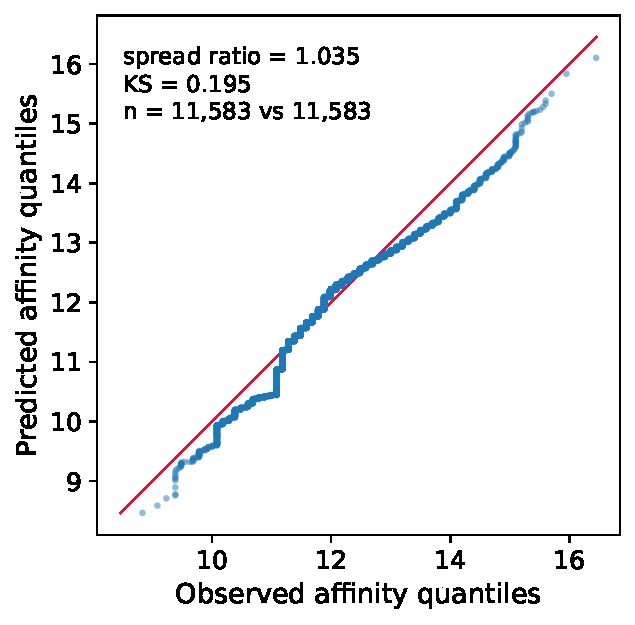
\includegraphics[width=\linewidth]{figs/oracles/kiba/BaselineOracle_qq_predicted.pdf}
        \caption{Baseline oracle}\label{fig:qq_baseline}
    \end{subfigure}
    \hfill
    \begin{subfigure}{0.32\textwidth}
        \centering
        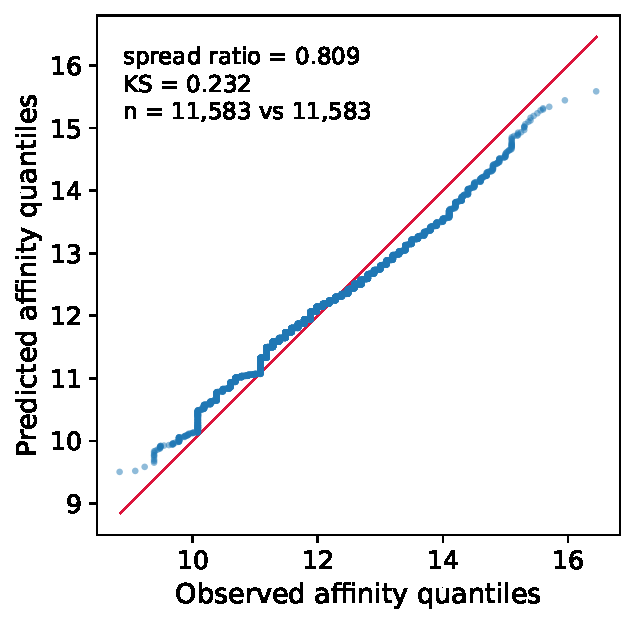
\includegraphics[width=\linewidth]{figs/oracles/kiba/GraphDTAOracle_qq_predicted.pdf}
        \caption{GraphDTA}\label{fig:qq_graphdta}
    \end{subfigure}
    \hfill
    \begin{subfigure}{0.32\textwidth}
        \centering
        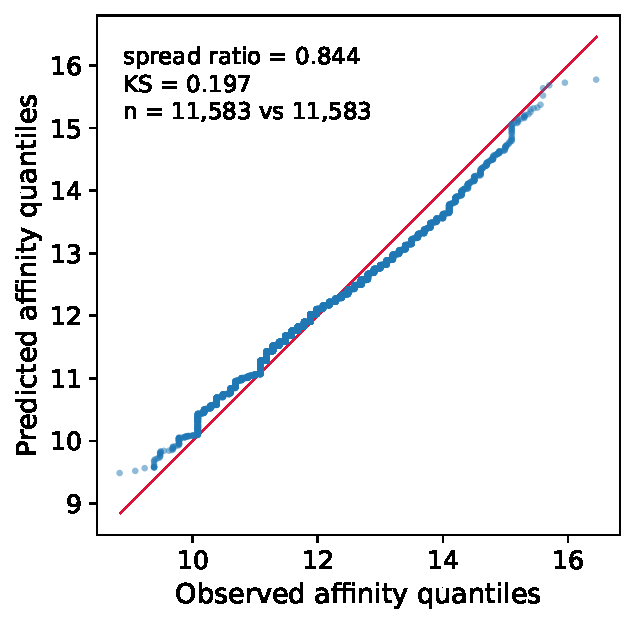
\includegraphics[width=\linewidth]{figs/oracles/kiba/GSDTAOracle_qq_predicted.pdf}
        \caption{GSDTA}\label{fig:qq_gsdta}
    \end{subfigure}

    \caption[QQ-plots of predicted and observed affinity values.]{QQ-plots comparing predicted and observed affinity values on KIBA for \textbf{(a)} the baseline oracle, \textbf{(b)} GraphDTA and \textbf{(c)} GSDTA. Corresponding quantiles show how the predicted affinity distribution relates to the observed one across its range, including the low- and high-affinity extremes.}
    \label{fig:three_figures}
\end{figure}

For a generated molecule, there is no measured affinity against which to calculate an error. It is still possible to ask whether the three oracles agree. Figure \ref{fig:or_disagree} measures their disagreement as the standard deviation of their predictions for a drug-protein pair, and relates it to chemical similarity and to prediction error on held-out measured pairs.

Generated molecules show greater disagreement than training molecules in KIBA and Davis, while these distributions overlap more in BindingDB and Papyrus. Disagreement decreases as similarity to the nearest training molecule increases: the Spearman correlations are $-0.545$, $-0.662$, $-0.127$ and $-0.145$ for KIBA, Davis, BindingDB and Papyrus, respectively. The relationship with unfamiliar chemistry is therefore more pronounced in the two denser datasets.

On measured held-out pairs, disagreement is positively associated with absolute prediction error, with correlations of $0.275$, $0.405$, $0.329$ and $0.356$ in the same dataset order. Together, these observations provide a reason to interpret predictions more cautiously when the oracles disagree, particularly for molecules less similar to training drugs.

\begin{figure}[H]
    \centering
    \sidepanel{figs/e7/kiba/oracle_disagreement_panels.pdf}{KIBA}{fig:or_disagree_kiba}
    \sidepanel{figs/e7/davis/oracle_disagreement_panels.pdf}{Davis}{fig:or_disagree_davis}
    \sidepanel{figs/e7/bindingdb/oracle_disagreement_panels.pdf}{BindingDB}{fig:or_disagree_bindingdb}
    \sidepanel{figs/e7/papyrus/oracle_disagreement_panels.pdf}{Papyrus}{fig:or_disagree_papyrus}
    \caption[Factors correlated with oracle disagreement.]{Oracle disagreement in
        \textbf{(a)} KIBA, \textbf{(b)} Davis, \textbf{(c)} BindingDB and \textbf{(d)} Papyrus.
        Disagreement is the standard deviation of the three oracle predictions for one
        drug-protein pair. The left panel compares the disagreement
        recorded on generated molecules with that recorded on training molecules. The middle panel asks whether
        disagreement tracks how unfamiliar a molecule is, measuring familiarity as the Tanimoto
        similarity of a generated molecule to the nearest molecule in the training set. The
        right panel asks whether disagreement tracks error. In both
        of the right-hand panels the generated molecules or measured pairs are sorted by
        disagreement and split into ten bins of equal count: each marker is one bin, at the mean
        disagreement of its members and the mean Tanimoto similarity or root mean squared error
        within it. The shaded band is a $95\%$ cluster bootstrap interval that resamples
        proteins.}
    \label{fig:or_disagree}
\end{figure}

\subsection{SelVAEGen improves selectivity over competing methods}\label{sec:main}
We now compare SelVAEGen with the three protein-targeted generators described in Section \ref{sec:literature}. All three were published in 2025 and are retrained from scratch for this comparison. The question is whether conditioning on a protein leads each model to generate molecules that preferentially bind to that protein.

Each model generates $256$ molecules for every protein in a dataset's test split. These proteins are unseen during generator training. The same oracle panel scores the generated molecules against their intended targets and the off-target proteins, and the experiment is repeated over independent seeds controlling the split and parameter initialization. Architecture and hyperparameter choices use the validation set, as described in Section \ref{sec:temp}.

SelVAEGen is the only model with significantly positive utility on all four datasets, and it shows the strongest overall preference for its conditioning proteins. We examine this result together with generation quality and chemical properties, then use the complementary selectivity metrics to describe the advantage in more detail. This order allows the selectivity results to be read together with the quality of the output from which they were calculated. The numerical examples below refer to KIBA, since most of the analysis remains valid in all cases. The figures present all four datasets.

Figure \ref{fig:e6_qual} reports validity, uniqueness and novelty. On KIBA, SelVAEGen and DeepDTAGen generate almost exclusively valid molecules, with validity $1.000$ and $0.976$, compared with $0.380$ for Prot2Drug and $0.322$ for ZeroGEN. The pattern differs for uniqueness and novelty. SelVAEGen has the lowest uniqueness, $0.446$, compared with $0.667$, $0.888$ and $0.967$ for DeepDTAGen, Prot2Drug and ZeroGEN. Its novelty is $0.275$, below the $0.634$ of Prot2Drug and $0.911$ of ZeroGEN, but above the $0.027$ of DeepDTAGen. Thus, SelVAEGen reliably produces valid structures but repeats molecules and recovers training examples more often than Prot2Drug and ZeroGEN. Those two models, in turn, fail to produce valid structures in most attempts.

\begin{figure}[H]
    \centering
    \sidepanel{figs/e6/kiba/seq_quality.pdf}{KIBA}{fig:e6_qual_kiba}
    \sidepanel{figs/e6/davis/seq_quality.pdf}{Davis}{fig:e6_qual_davis}
    \sidepanel{figs/e6/bindingdb/seq_quality.pdf}{BindingDB}{fig:e6_qual_bindingdb}
    \sidepanel{figs/e6/papyrus/seq_quality.pdf}{Papyrus}{fig:e6_qual_papyrus}
    \caption[Generation quality of the four models, by dataset.]{Validity, uniqueness and novelty of generated molecules in \textbf{(a)} KIBA, \textbf{(b)} Davis, \textbf{(c)} BindingDB and \textbf{(d)} Papyrus. Each row corresponds to results of the dataset mentioned in the left. Validity measures how often a generation attempt produces a parsable molecule, uniqueness measures how much of the valid output is distinct, and novelty measures how much is absent from the training set. All four models were trained from scratch on the same splits with the same tokenizer.}
    \label{fig:e6_qual}
\end{figure}

Figures \ref{fig:e6_chema} and \ref{fig:chemb} examine predicted affinity and chemical quality. On KIBA, SelVAEGen has the highest mean predicted on-target affinity, $12.440$, compared with $11.470$, $11.418$ and $11.201$ for the competing models. It also has the highest mean affinity in the top decile, $14.010$. Its success rate of $0.020$ is close to the $0.021$ of Prot2Drug and exceeds the $0.001$ of DeepDTAGen. The Fr\'echet ChemNet distance is lowest for SelVAEGen, at $2.536$ compared with $4.559$, $6.113$ and $6.325$, indicating that its generated distribution is closest to the training chemistry under this measure.

The per-molecule chemical scores reveal a different aspect of the output. SelVAEGen's Lipinski compliance of $0.916$ and QED of $0.524$ are the lowest among the four models, while its synthetic accessibility score of $2.855$ is the least favorable. Higher predicted affinity and a smaller distance from the training distribution therefore coexist with less favorable values on these chemical criteria.

\begin{figure}[H]
    \centering
    \sidepanel{figs/e6/kiba/seq_potency.pdf}{KIBA}{fig:e6_chema_kiba}
    \sidepanel{figs/e6/davis/seq_potency.pdf}{Davis}{fig:e6_chema_davis}
    \sidepanel{figs/e6/bindingdb/seq_potency.pdf}{BindingDB}{fig:e6_chema_bindingdb}
    \sidepanel{figs/e6/papyrus/seq_potency.pdf}{Papyrus}{fig:e6_chema_papyrus}
    \caption[Potency of the generated molecules, by dataset.]{Predicted potency and distributional similarity of generated molecules in \textbf{(a)} KIBA, \textbf{(b)} Davis, \textbf{(c)} BindingDB and \textbf{(d)} Papyrus. Mean predicted affinity summarizes the whole library, while the mean of the top decile summarizes its best tenth, the candidates of greatest interest for subsequent selection. Success rate counts unique, novel molecules whose predicted affinity clears the dataset threshold, marked by a dashed line in the first two panels. Fr\'echet ChemNet distance compares the generated and training chemical distributions; lower values indicate a closer match, making this the only panel where lower is better. BindingDB and Papyrus provide roughly three measurements per drug, so their affinity estimates draw on sparser data than KIBA and Davis.}
    \label{fig:e6_chema}
\end{figure}

\begin{figure}[H]
    \centering
    \sidepanel{figs/e6/kiba/seq_chemistry.pdf}{KIBA}{fig:chemb_kiba}
    \sidepanel{figs/e6/davis/seq_chemistry.pdf}{Davis}{fig:chemb_davis}
    \sidepanel{figs/e6/bindingdb/seq_chemistry.pdf}{BindingDB}{fig:chemb_bindingdb}
    \sidepanel{figs/e6/papyrus/seq_chemistry.pdf}{Papyrus}{fig:chemb_papyrus}
    \caption[Chemical properties of the generated molecules, by dataset.]{Chemical properties of generated molecules in \textbf{(a)} KIBA, \textbf{(b)} Davis, \textbf{(c)} BindingDB and \textbf{(d)} Papyrus. Lipinski compliance is the fraction meeting the rule-of-five criterion for molecular size, lipophilicity and hydrogen bonding. QED summarizes drug-likeness on a scale of $[0,1]$. The synthetic accessibility score estimates the difficulty of making a molecule, from $1$ to $10$, and is the only panel where lower is better. Internal diversity is the mean pairwise structural dissimilarity within a generated library; low values indicate that its molecules are structurally similar among themselves.}
    \label{fig:chemb}
\end{figure}

The central comparison concerns selectivity. The $\Delta$ score measures the mean on-target affinity advantage, while Directional Consistency asks how often that advantage occurs in individual comparisons. Reading them together helps distinguish a systematic preference from an average driven by a few extreme molecules.

On KIBA, SelVAEGen obtains a $\Delta$ score of $0.2887$, compared with $0.0186$, $0.0049$ and $-0.0028$ for Prot2Drug, ZeroGEN and DeepDTAGen, respectively (Figure \ref{fig:e6_sel}). The slightly negative value for DeepDTAGen means that its off-target predictions are, on average, marginally higher than its on-target predictions. SelVAEGen also reaches a Directional Consistency of $0.6297$, whereas the baselines range from $0.4986$ to $0.5052$, close to the chance reference of $0.5$ (Figure \ref{fig:e6_agree}). Its average advantage is therefore accompanied by a more frequent preference for the conditioning protein.

\begin{figure}[H]
    \centering
    \sidepanel{figs/e6/kiba/seq_agreement.pdf}{KIBA}{fig:e6_agree_kiba}
    \sidepanel{figs/e6/davis/seq_agreement.pdf}{Davis}{fig:e6_agree_davis}
    \sidepanel{figs/e6/bindingdb/seq_agreement.pdf}{BindingDB}{fig:e6_agree_bindingdb}
    \sidepanel{figs/e6/papyrus/seq_agreement.pdf}{Papyrus}{fig:e6_agree_papyrus}
    \caption[Directional Consistency and Tanimoto Gap, by dataset.]{Directional Consistency and Tanimoto Gap in \textbf{(a)} KIBA, \textbf{(b)} Davis, \textbf{(c)} BindingDB and \textbf{(d)} Papyrus. Directional Consistency counts how often a molecule's predicted on-target affinity exceeds its affinity for an individual off-target protein. It therefore shows whether the on-target advantage occurs regularly, without being dominated by a few extreme $\Delta$ scores. The dashed line marks the chance level of $0.5$. Tanimoto Gap measures the excess structural similarity between molecules generated for the same protein over those generated for different proteins. Its reference value of $0$ indicates no systematic structural dependence on the target.}
    \label{fig:e6_agree}
\end{figure}

The Tanimoto Gap asks whether this dependence on the target is also visible in molecular structure. SelVAEGen obtains $0.0556$, compared with $0.0324$, $0.0064$ and $-0.0002$ for the baselines (Figure \ref{fig:e6_agree}). Molecules generated for the same protein are consequently more similar to one another than to molecules generated for different proteins. This provides a chemical counterpart to the affinity comparisons.

Effective $\Delta$ then accounts for generation attempts that fail the validity, uniqueness, novelty or on-target affinity requirements defined in Chapter \ref{sec:metrics}. SelVAEGen retains the highest score, $0.0954$, compared with $0.0408$, $0.0290$ and $0.0170$, although the difference between models is narrower (Figure \ref{fig:e6_sel}). The gain in predicted selectivity thus remains under the more restrictive measure of useful output per generation attempt.

\begin{figure}[H]
    \centering
    \sidepanel{figs/e6/kiba/seq_deltas.pdf}{KIBA}{fig:e6_sel_kiba}
    \sidepanel{figs/e6/davis/seq_deltas.pdf}{Davis}{fig:e6_sel_davis}
    \sidepanel{figs/e6/bindingdb/seq_deltas.pdf}{BindingDB}{fig:e6_sel_bindingdb}
    \sidepanel{figs/e6/papyrus/seq_deltas.pdf}{Papyrus}{fig:e6_sel_papyrus}
    \caption[The three $\Delta$ metrics, by dataset.]{The three $\Delta$ metrics in \textbf{(a)} KIBA, \textbf{(b)} Davis, \textbf{(c)} BindingDB and \textbf{(d)} Papyrus. The $\Delta$ score is the mean difference between a generated molecule's predicted affinity for its intended target and its mean affinity for the alternatives. Distributional $\Delta$ compares the complete on-target and off-target affinity distributions, without pairing each molecule with its own off-target values. Effective $\Delta$ combines selectivity with validity, uniqueness and novelty, accounting for generation attempts that do not yield usable new molecules. The dashed line marks the reference value of $0$ for a generator that ignores its conditioning protein.}
    \label{fig:e6_sel}
\end{figure}

The same result can be examined across the distribution of individual molecules. Figure \ref{fig:cum} reports, for each level of selectivity, the fraction of generated molecules whose $\delta$ exceeds that level. Reading a curve at $\delta=0$ shows how often a molecule favors its target over its average off-target affinity, and moving to the right imposes a larger required advantage. It can be seen that SelVAEGen has a uniformly higher fraction of molecules exceeding each selectivity threshold compared with the competitors.

\begin{figure}[hp]
    \centering
    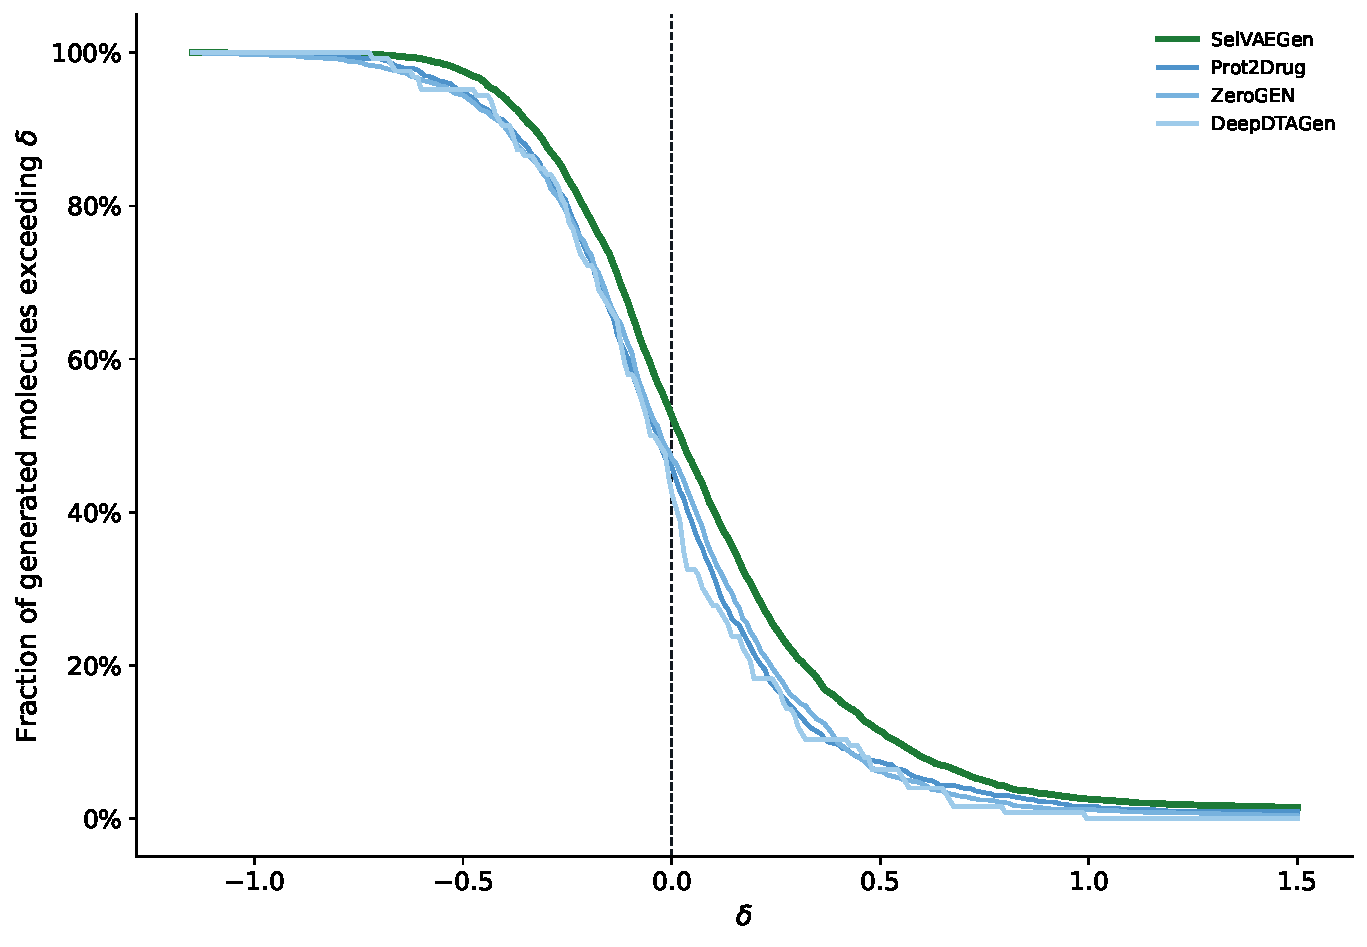
\includegraphics[width=\linewidth]{figs/e7/kiba/delta_survival.pdf}
    \caption[Fraction of generated drugs above a level of selectivity.]{Fraction of generated KIBA molecules whose individual selectivity score exceeds the value $\delta$ on the horizontal axis. The curves decrease as the required selectivity increases. The dashed vertical line marks $\delta=0$, where a molecule's predicted affinity for its intended target equals its mean predicted affinity for the other proteins.}
    \label{fig:cum}
\end{figure}

We next return to the threshold-dependent definition of utility in Section \ref{sec:defs}. Figure \ref{fig:kdes} shows the on-target and off-target affinity distributions, and Table \ref{tab:integrals} reports the difference between their estimated probabilities above the dataset threshold. This asks whether a generated molecule is more likely to exceed the binding threshold for its intended target than for an alternative protein. SelVAEGen is the only model whose on-target distribution is consistently shifted towards higher affinities across all four datasets, resulting in the blue areas in Figure \ref{fig:kdes} corresponding to the utility of the generator.

\begin{figure}[hp]
    \centering
    \sidepanel{figs/e6/kiba/models_side_by_side.pdf}{KIBA}{fig:kdes_kiba}
    \sidepanel{figs/e6/davis/models_side_by_side.pdf}{Davis}{fig:kdes_davis}
    \sidepanel{figs/e6/bindingdb/models_side_by_side.pdf}{BindingDB}{fig:kdes_bindingdb}
    \sidepanel{figs/e6/papyrus/models_side_by_side.pdf}{Papyrus}{fig:kdes_papyrus}
    \caption[On- and off-target affinity distributions, by dataset.]{Estimated densities of on-target and off-target predicted affinities in \textbf{(a)} KIBA, \textbf{(b)} Davis, \textbf{(c)} BindingDB and \textbf{(d)} Papyrus. Each model's two curves represent $p_G$ and $q_G$ from Section \ref{sec:defs}. An on-target distribution shifted towards higher affinity values indicates target preference. SelVAEGen shows this shift consistently across all four datasets. Integrating the difference between the densities above the dataset's positive-affinity threshold gives the utility estimates in Table \ref{tab:integrals}. The blue are corresponds to the utility of the generator.}
    \label{fig:kdes}
\end{figure}

SelVAEGen obtains utility values of $0.1334$, $0.2013$, $0.0275$ and $0.0373$ on KIBA, Davis, BindingDB and Papyrus, respectively. These are excess probabilities of an above-threshold on-target affinity relative to an off-target affinity. Its utility is significantly above zero on all four datasets under a $t$-test after Benjamini-Hochberg (BH) correction for multiple comparisons \parencite{benjamini1995controlling}. Some baselines also have significantly positive utility on individual datasets, particularly KIBA, but their effects are substantially smaller. Under the definition in Section \ref{sec:defs}, SelVAEGen is therefore the only model with consistent evidence of selective generation across all datasets considered here.

\begin{table}[ht]
    \centering
    \caption[Selectivity estimates across datasets.]{Selectivity utility above each dataset's positive-affinity threshold, estimated by numerical integration, and Distributional $\Delta$ scores. Values are mean $\pm$ standard deviation across replication seeds. Bold values indicate means significantly above zero under a one-tailed $t$-test after Benjamini-Hochberg correction at a false discovery rate of $q=0.05$.}
    \label{tab:integrals}
    \begin{tabular}{llcc}
        \toprule
        Dataset & Model
        & Utility
        & Distributional $\Delta$ score \\
        \midrule

        KIBA & SelVAEGen
        & \textbf{0.1334 $\pm$ 0.0499}
        & 0.1771 $\pm$ 0.0978 \\
        KIBA & DeepDTAGen
        & \textbf{0.0045 $\pm$ 0.0016}
        & -0.0145 $\pm$ 0.0427 \\
        KIBA & Prot2Drug
        & \textbf{0.0165 $\pm$ 0.0017}
        & 0.0278 $\pm$ 0.0517 \\
        KIBA & ZeroGEN
        & \textbf{0.0046 $\pm$ 0.0024}
        & 0.0234 $\pm$ 0.0183 \\
        \midrule

        Davis & SelVAEGen
        & \textbf{0.2013 $\pm$ 0.0375}
        & 1.2521 $\pm$ 0.6767 \\
        Davis & DeepDTAGen
        & -0.0002 $\pm$ 0.0004
        & -0.0695 $\pm$ 0.0073 \\
        Davis & Prot2Drug
        & 0.0001 $\pm$ 0.0015
        & -0.0705 $\pm$ 0.0095 \\
        Davis & ZeroGEN
        & 0.0012 $\pm$ 0.0011
        & -0.0303 $\pm$ 0.0256 \\
        \midrule

        BindingDB & SelVAEGen
        & \textbf{0.0275 $\pm$ 0.0050}
        & 0.0170 $\pm$ 0.0129 \\
        BindingDB & DeepDTAGen
        & \textbf{0.0060 $\pm$ 0.0026}
        & -0.0278 $\pm$ 0.0160 \\
        BindingDB & Prot2Drug
        & -0.0001 $\pm$ 0.0086
        & -0.0615 $\pm$ 0.0443 \\
        BindingDB & ZeroGEN
        & 0.0063 $\pm$ 0.0116
        & -0.0541 $\pm$ 0.0316 \\
        \midrule

        Papyrus & SelVAEGen
        & \textbf{0.0373 $\pm$ 0.0222}
        & 0.0298 $\pm$ 0.0533 \\
        Papyrus & DeepDTAGen
        & -0.0023 $\pm$ 0.0019
        & -0.0320 $\pm$ 0.0255 \\
        Papyrus & Prot2Drug
        & 0.0040 $\pm$ 0.0132
        & 0.0005 $\pm$ 0.0719 \\
        Papyrus & ZeroGEN
        & -0.0004 $\pm$ 0.0057
        & -0.0320 $\pm$ 0.0053 \\

        \bottomrule
    \end{tabular}
\end{table}

Figure \ref{fig:utility} extends this comparison by varying the affinity threshold. At each point on a curve, utility compares the fractions of on-target and off-target predictions exceeding that value. The vertical dashed line recovers the threshold used in Table \ref{tab:integrals}. This view shows how much the conclusion depends on the chosen threshold, while the $\Delta$ score summarizes utility across thresholds as established in Chapter \ref{sec:metrics}. As before, SelVAEGen consistently demonstrates superior utility across the range of thresholds.

\clearpage
\begin{figure}[H]
    \centering
    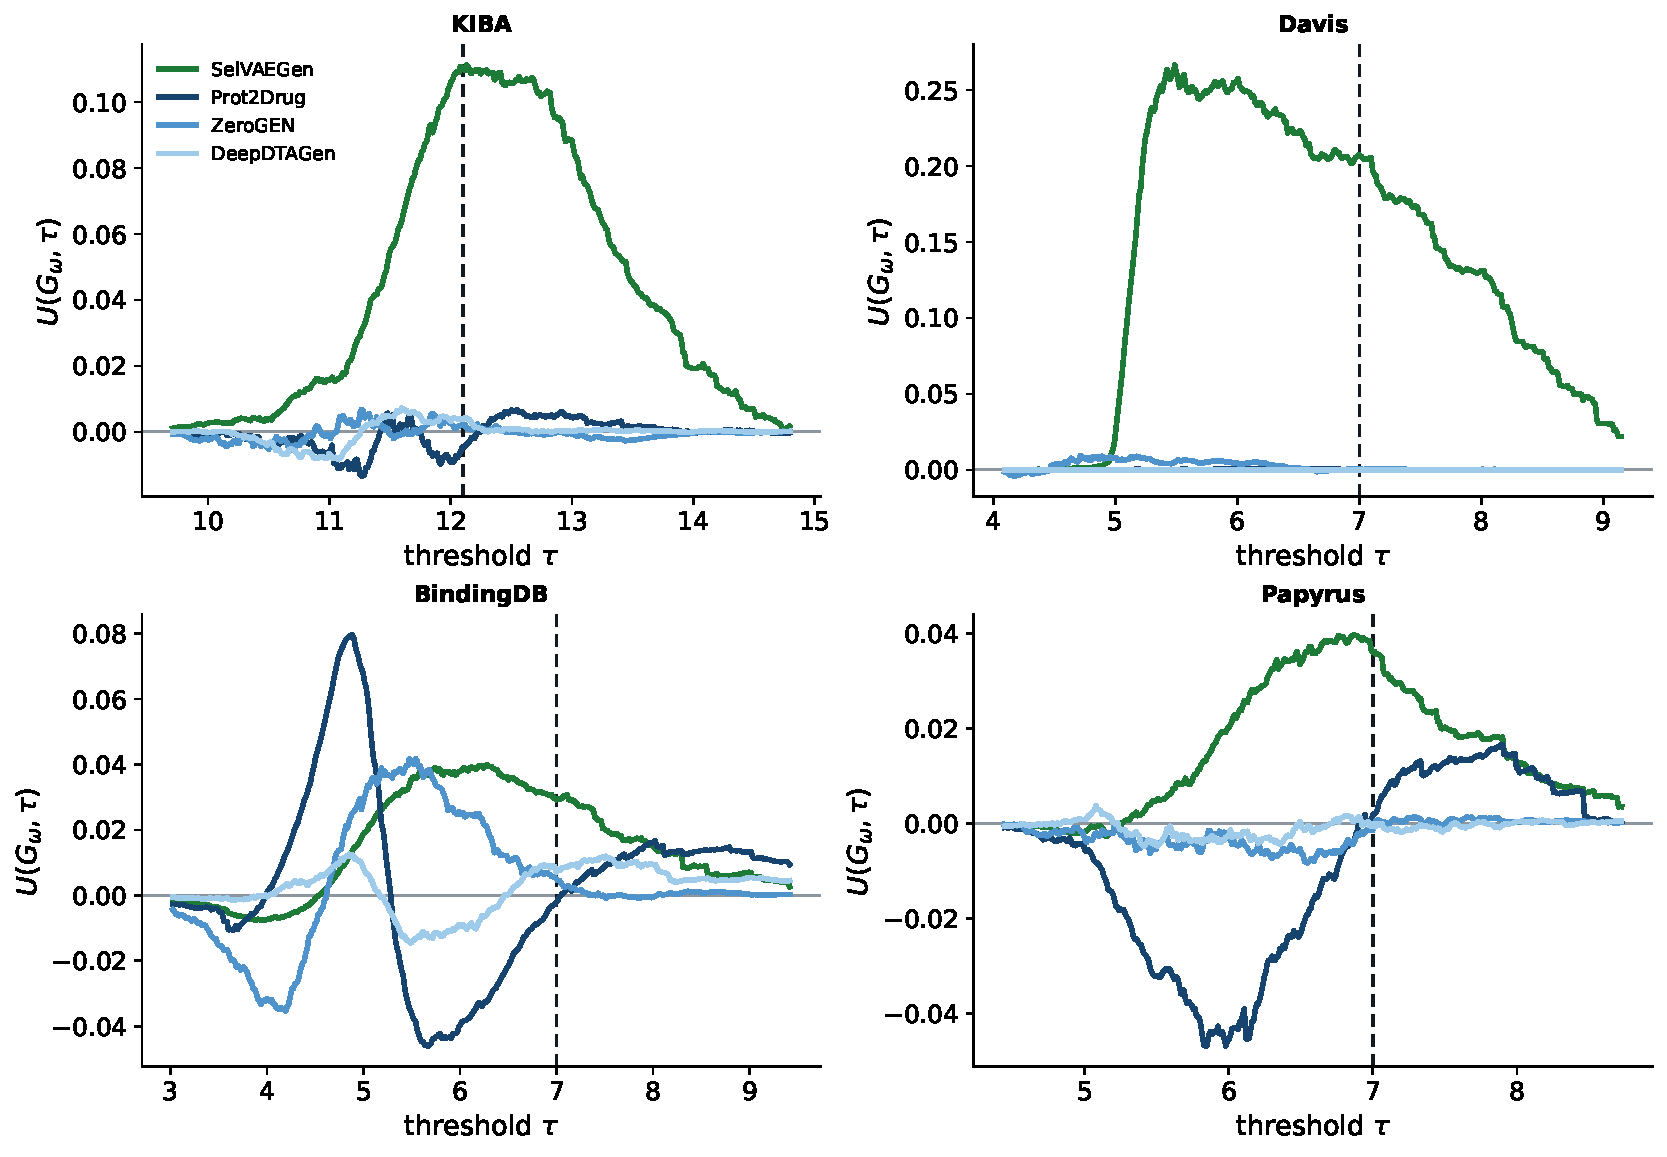
\includegraphics[width=\textwidth]{figs/e7/utility_curves.pdf}
    \caption[Utility at every threshold, by dataset.]{Selectivity utility $U(G_\omega,\tau)$ across affinity thresholds, mean over seeds. At each threshold $\tau$, utility is the excess probability of an above-threshold affinity for the intended target compared with an off-target protein. Values above zero indicate target preference at that threshold. A curve remaining above zero across the range indicates that the advantage persists as the threshold changes. The dashed vertical line marks the threshold used in Table \ref{tab:integrals}. These curves use empirical distributions.}
    \label{fig:utility}
\end{figure}

\subsection{What SelVAEGen generates}
The preceding metrics summarize complete generated libraries. We now examine individual molecules and target-specific groups to see how those aggregate patterns appear in the output. The examples illustrate molecular structure, predicted affinity and dependence on the conditioning protein.

Figure \ref{fig:e7_affinity} compares two affinity distributions for each of 20 KIBA random test proteins: the measured affinities of the dataset's drugs and the predicted affinities of the molecules generated for that target. For 19 of the 20 proteins, the generated mean is higher than the measured mean. Across the twenty proteins, the corresponding averages are $12.391$ and $11.694$.

Figure \ref{fig:e7_affinity_others} repeats the analysis on the remaining datasets. The mean generated-minus-measured difference over twenty proteins is $1.217$ on Davis and $0.697$ on KIBA, compared with $0.164$ on BindingDB and $0.148$ on Papyrus. The larger shifts occur in the datasets that provide more selectivity comparisons per molecule, following the pattern described in Section \ref{sec:datasets}.

\begin{figure}[H]
    \centering
    
\includegraphics[width=\linewidth]{figs/e7/kiba/affinity.pdf}
    \caption[Affinity of observed and generated drugs in KIBA.]{Measured affinities of KIBA drugs and predicted affinities of SelVAEGen molecules for twenty held-out test proteins. Each column contains a pair of distributions for one protein: measured affinities on the left and generated-molecule predictions on the right. Proteins are ordered by mean measured affinity, so the red boxes rise from left to right by construction. The generated mean exceeds the measured mean for 19 of the 20 proteins. The two sides represent experimental observations and oracle predictions, respectively, with the oracles trained on affinity measurements of the same kind as those on the left.}
    \label{fig:e7_affinity}
\end{figure}

\begin{figure}[H]
    \centering
    \sidepanel{figs/e7/davis/affinity.pdf}{Davis}{fig:e7_aff_davis}
    \sidepanel{figs/e7/bindingdb/affinity.pdf}{BindingDB}{fig:e7_aff_bindingdb}
    \sidepanel{figs/e7/papyrus/affinity.pdf}{Papyrus}{fig:e7_aff_papyrus}
    \caption[Affinity of observed and generated drugs in Davis, BindingDB and Papyrus.]{Measured and generated-molecule affinity distributions in \textbf{(a)} Davis, \textbf{(b)} BindingDB and \textbf{(c)} Papyrus, using the same presentation as Figure \ref{fig:e7_affinity}. Each column is one held-out test protein, with measured affinities of dataset drugs on the left and predicted affinities of SelVAEGen molecules on the right. Proteins are ordered within each row by mean measured affinity, so the red boxes rise from left to right by construction. Experimental observations are therefore compared with oracle predictions. The displacement between these distributions varies across datasets with different measurement densities.}
    \label{fig:e7_affinity_others}
\end{figure}

Figure \ref{fig:e7_affinity_models} applies the same comparison to the competing generators on KIBA. Using the same proteins and measured reference makes it possible to see whether the upward displacement also occurs for their generated libraries.

\begin{figure}[H]
    \centering
    \sidepanel{figs/e7/kiba/affinity_DeepDTAGen.pdf}{DeepDTAGen}{fig:e7_aff_comp_DeepDTAGen}
    \sidepanel{figs/e7/kiba/affinity_Prot2Drug.pdf}{Prot2Drug}{fig:e7_aff_comp_Prot2Drug}
    \sidepanel{figs/e7/kiba/affinity_ZeroGEN.pdf}{ZeroGEN}{fig:e7_aff_comp_ZeroGEN}
    \caption[Affinity of observed and generated drugs for the competing methods on KIBA.]{The KIBA comparison of Figure \ref{fig:e7_affinity} for \textbf{(a)} DeepDTAGen, \textbf{(b)} Prot2Drug and \textbf{(c)} ZeroGEN. Every row uses the same twenty proteins in the same order by mean measured affinity, so the red reference boxes are identical and column $i$ refers to the same protein throughout. Mean predicted affinities are $11.536$, $11.445$ and $11.212$, respectively, against a measured reference mean of $11.694$. The upward displacement seen for SelVAEGen is absent from these model averages.}
    \label{fig:e7_affinity_models}
\end{figure}

Figure \ref{fig:e7_tanimoto} examines how the conditioning protein changes molecular structure. The rows and columns contain generated molecules, with molecules produced for the same protein placed together. Higher similarity within one such group appears as a block along the diagonal. SelVAEGen shows this structure, consistent with its positive Tanimoto Gap: changing the target changes the region of chemical space from which molecules are generated.

The pattern must be read together with uniqueness and internal diversity. A model that always returned one fixed molecule for each protein would also produce strong diagonal blocks. The blocks show a dependence on the target; the generation-quality metrics indicate how much variation remains within each target's library.

\begin{figure}[H]
    \centering
    \begin{subfigure}{0.62\linewidth}
        \centering

        \begin{minipage}[c]{0.49\linewidth}
            \centering
            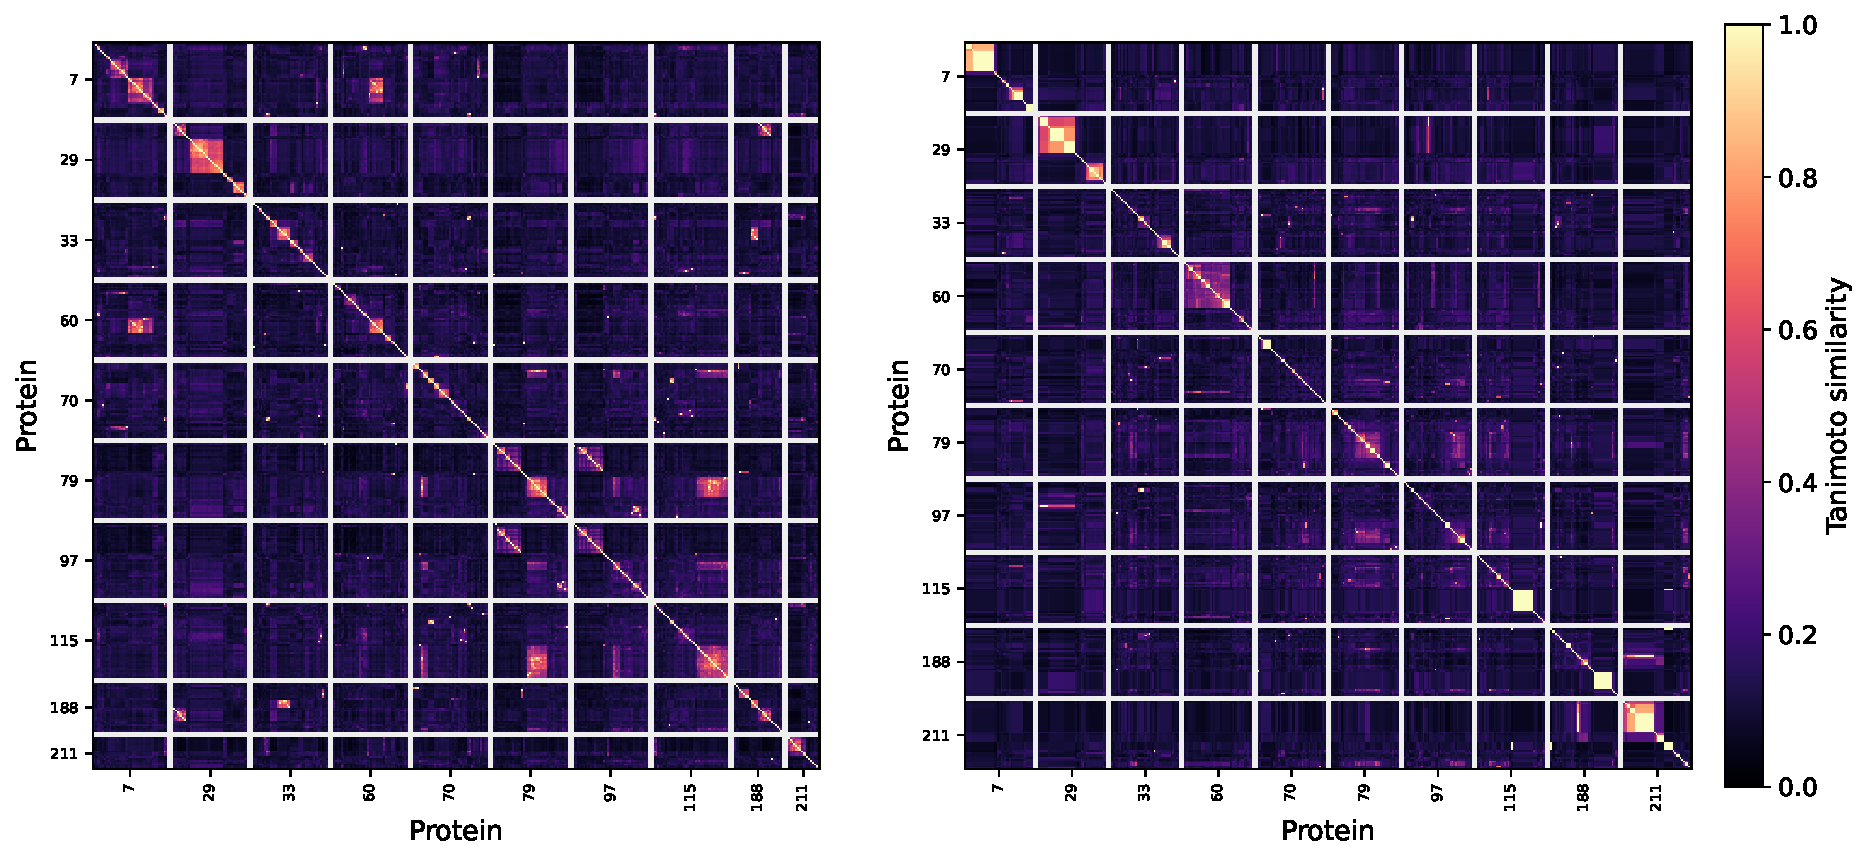
\includegraphics[
                trim=0 0 497bp 0,
                clip,
                width=\linewidth
            ]{figs/e7/kiba/tanimoto.pdf}
        \end{minipage}
        \hfill
        \begin{minipage}[c]{0.45\linewidth}
            \centering
            \caption{Training drugs}
            \label{fig:e7_tan_control}
        \end{minipage}

    \end{subfigure}

    \begin{subfigure}{0.41\linewidth}
        \centering
        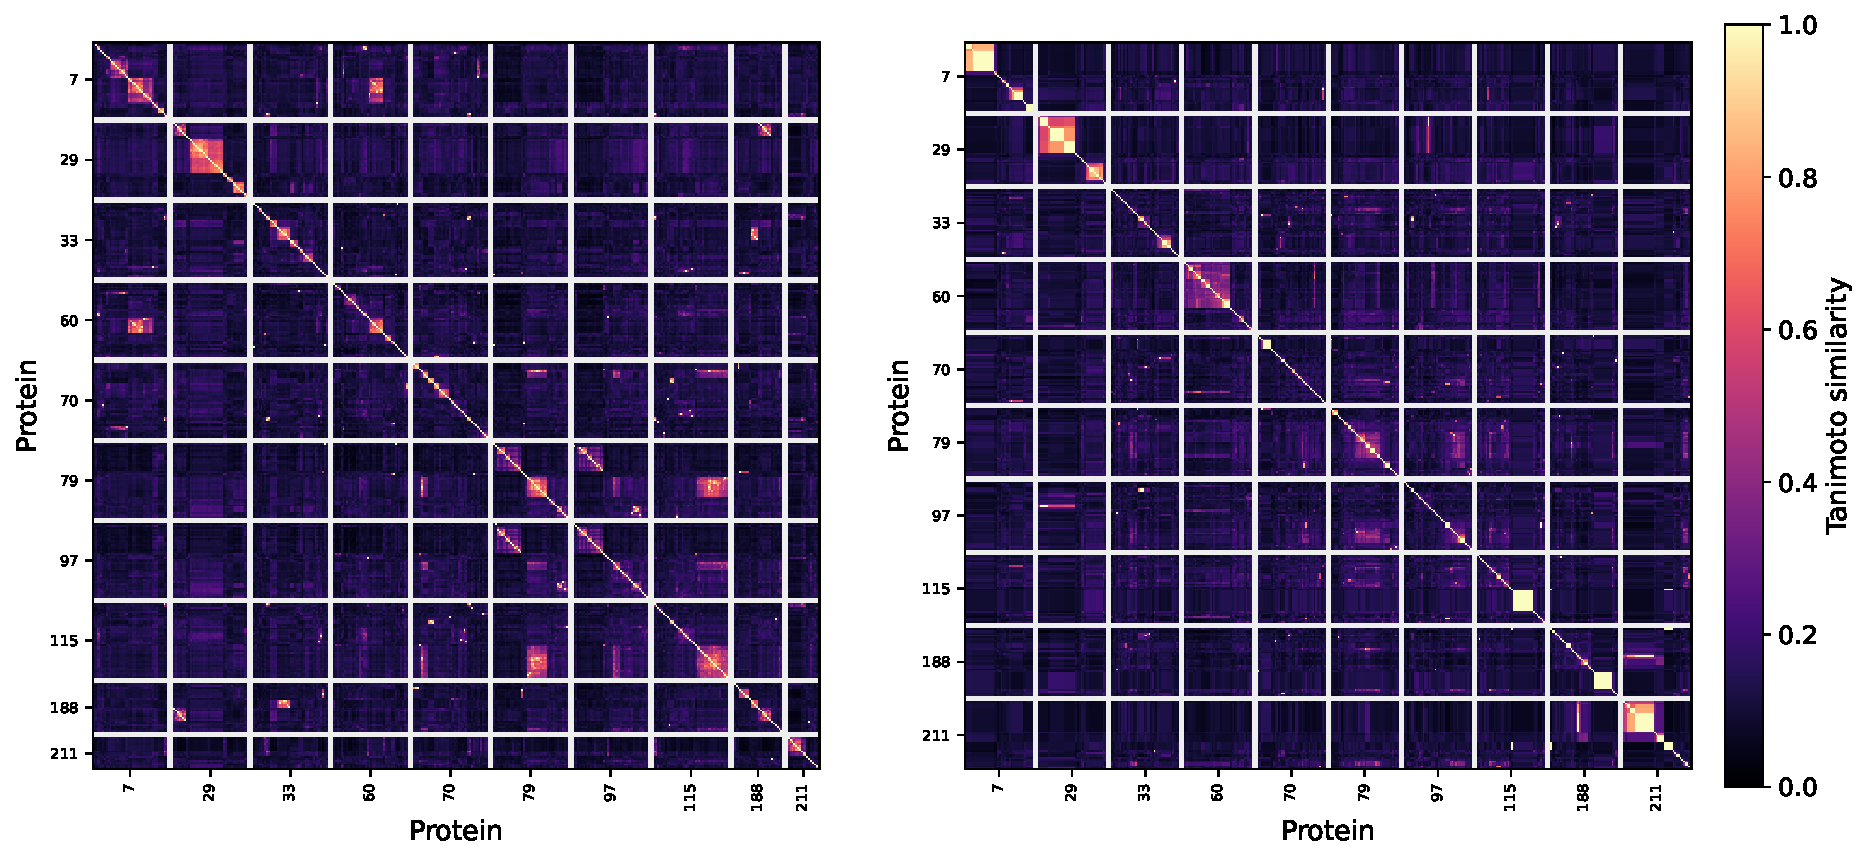
\includegraphics[trim=405bp 0 0 0, clip, width=\linewidth]{figs/e7/kiba/tanimoto.pdf}
        \caption{SelVAEGen}\label{fig:e7_tan_sel}
    \end{subfigure}
    \hfill
    \begin{subfigure}{0.41\linewidth}
        \centering
        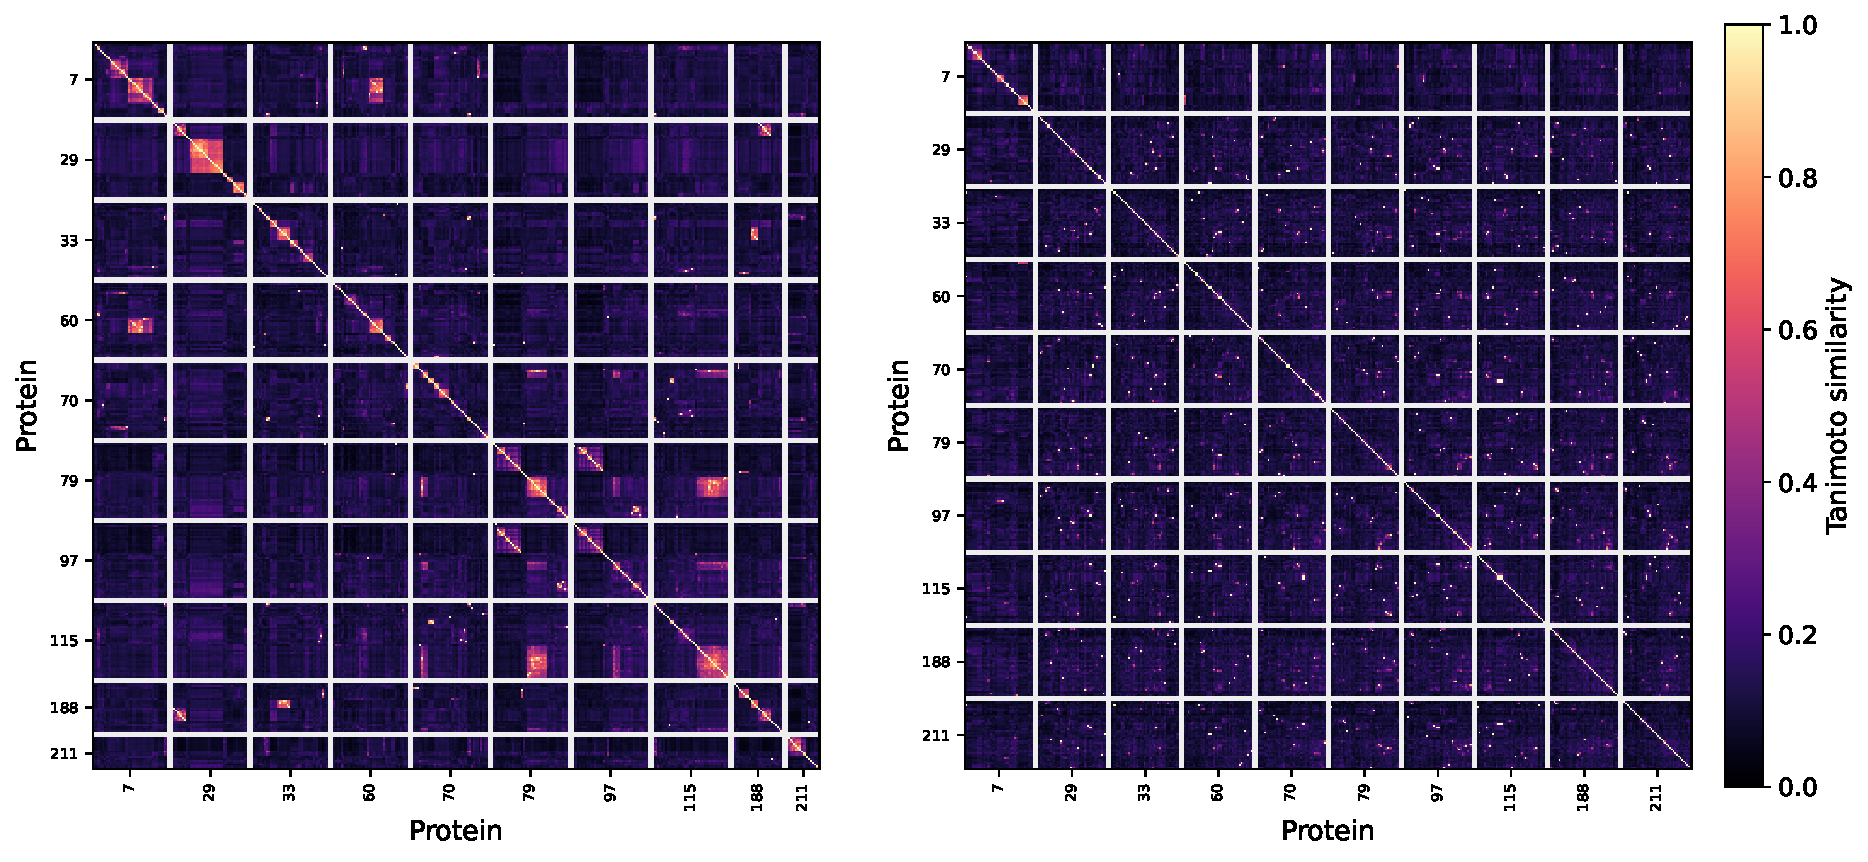
\includegraphics[trim=405bp 0 0 0, clip, width=\linewidth]{figs/e7/kiba/tanimoto_DeepDTAGen.pdf}
        \caption{DeepDTAGen}\label{fig:e7_tan_deep}
    \end{subfigure}

    \begin{subfigure}{0.41\linewidth}
        \centering
        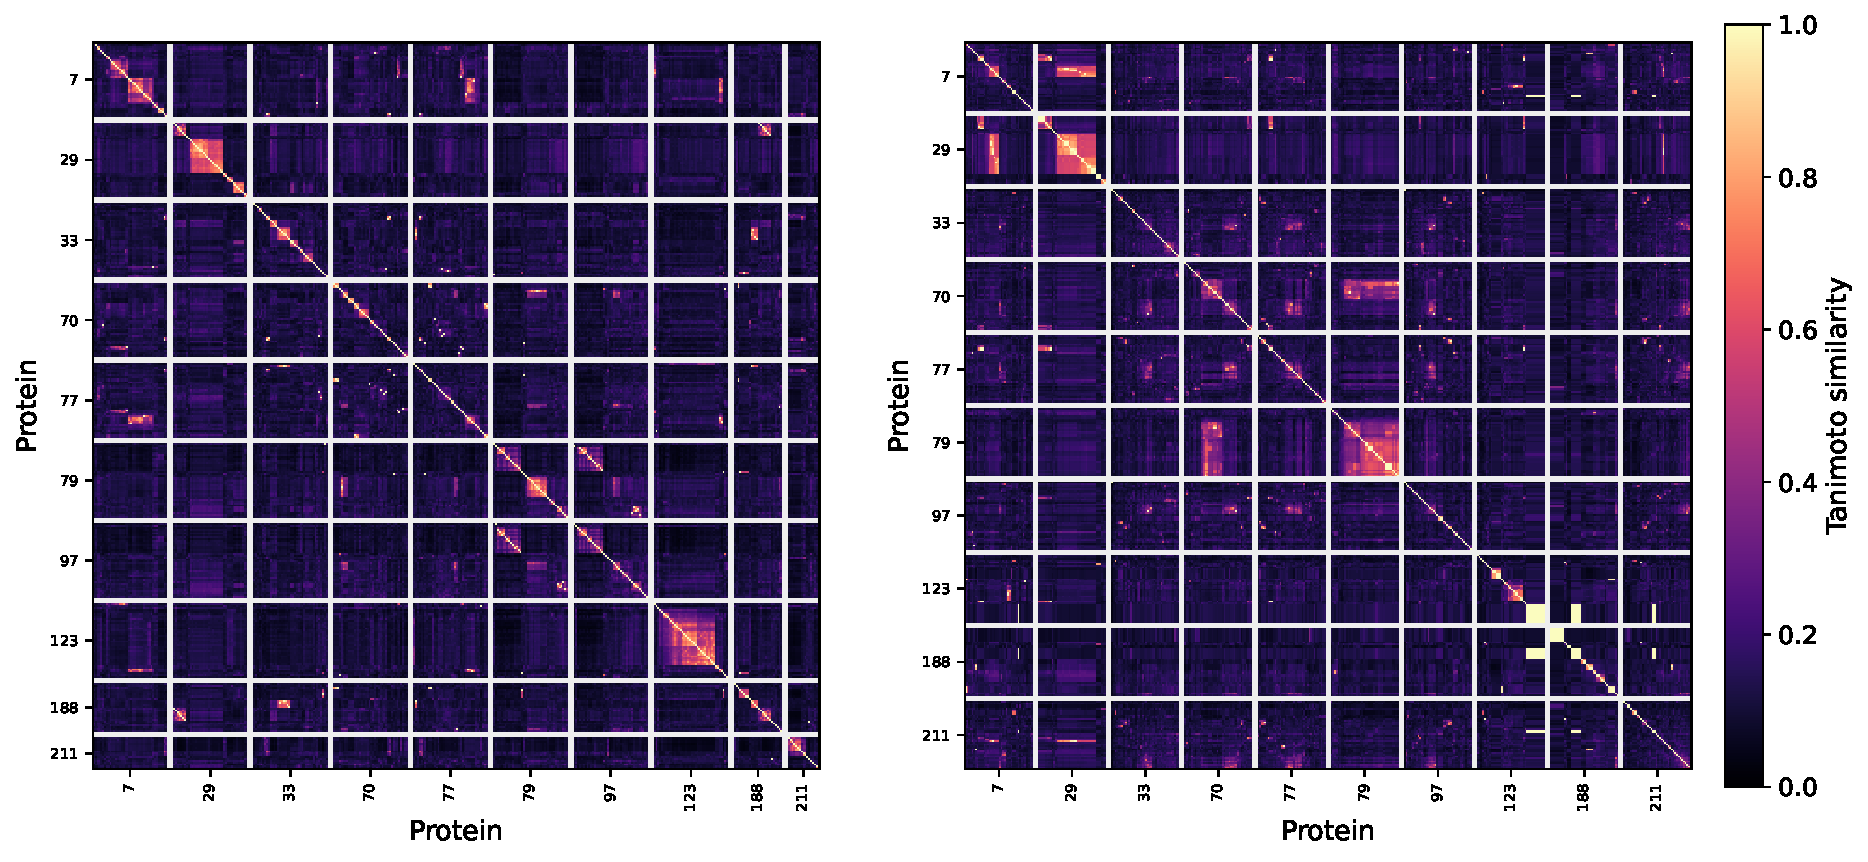
\includegraphics[trim=405bp 0 0 0, clip, width=\linewidth]{figs/e7/kiba/tanimoto_Prot2Drug.pdf}
        \caption{Prot2Drug}\label{fig:e7_tan_prot}
    \end{subfigure}
    \hfill
    \begin{subfigure}{0.41\linewidth}
        \centering
        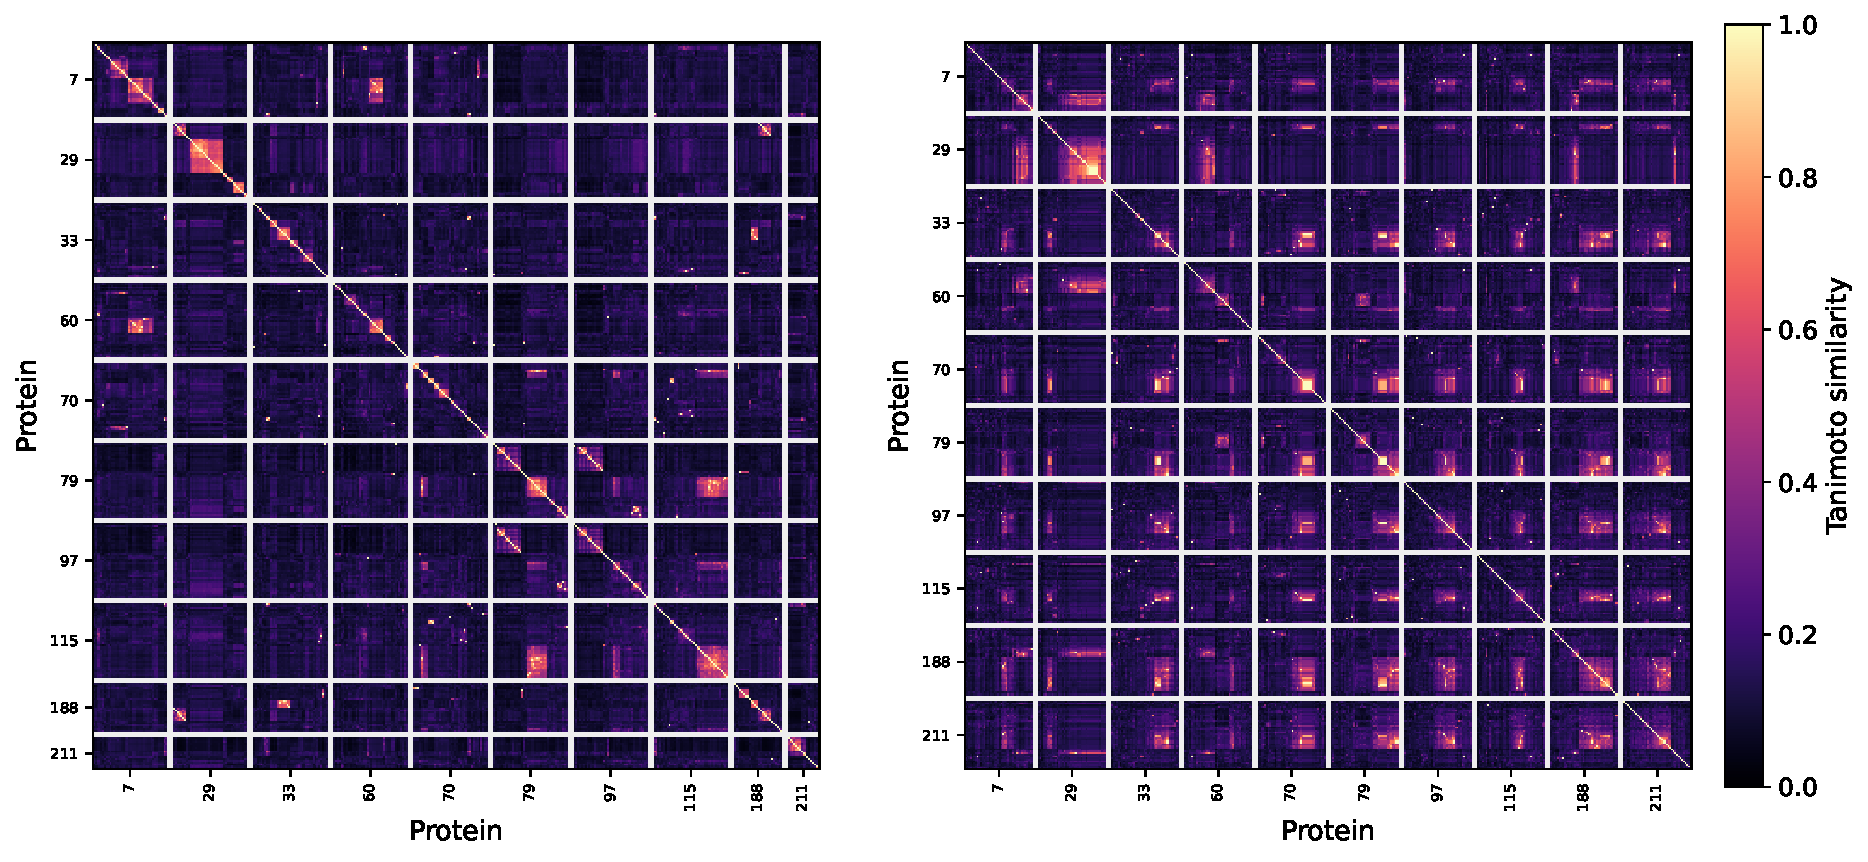
\includegraphics[trim=405bp 0 0 0, clip, width=\linewidth]{figs/e7/kiba/tanimoto_ZeroGEN.pdf}
        \caption{ZeroGEN}\label{fig:e7_tan_zero}
    \end{subfigure}
    \caption[Pairwise similarity of generated molecules, grouped by target.]{Pairwise Tanimoto similarity on KIBA, with molecules ordered so that those generated for the same protein are adjacent. This places within-target comparisons in blocks along the diagonal. \textbf{(a)} shows the dataset's drugs for ten proteins as a measured control, and \textbf{(b)} to \textbf{(e)} show the models' generated molecules on the same similarity scale. Stronger diagonal blocks indicate greater within-target than cross-target similarity, consistent with a positive Tanimoto Gap; DeepDTAGen shows no such structure. Repetition can also strengthen these blocks, which is why they must be read together with the diversity metrics.}
    \label{fig:e7_tanimoto}
\end{figure}

To illustrate how generated libraries could be used to select candidates, we consider 10 random test proteins and choose the novel molecule with the highest predicted selectivity for each target. Figure \ref{fig:e7_selectivity} places these molecules on the rows and the proteins on the columns. Each diagonal cell is therefore an on-target prediction, and the other cells in that row are predictions for the same molecule against alternative proteins. Gray values indicate predicted affinity values below the dataset's threshold, and green values indicate predicted affinity values above the threshold.

The desired pattern is a high diagonal value accompanied by lower off-diagonal values. In this way, the heatmap shows whether a selected molecule's predicted affinity is selective to its intended target. The pattern observed for SelVAEGen illustrates the individual candidates underlying its aggregate selectivity results. These are candidates identified by oracle scoring for possible further investigation.

\begin{figure}[H]
    \centering
    \begin{subfigure}{0.49\linewidth}
        \centering
        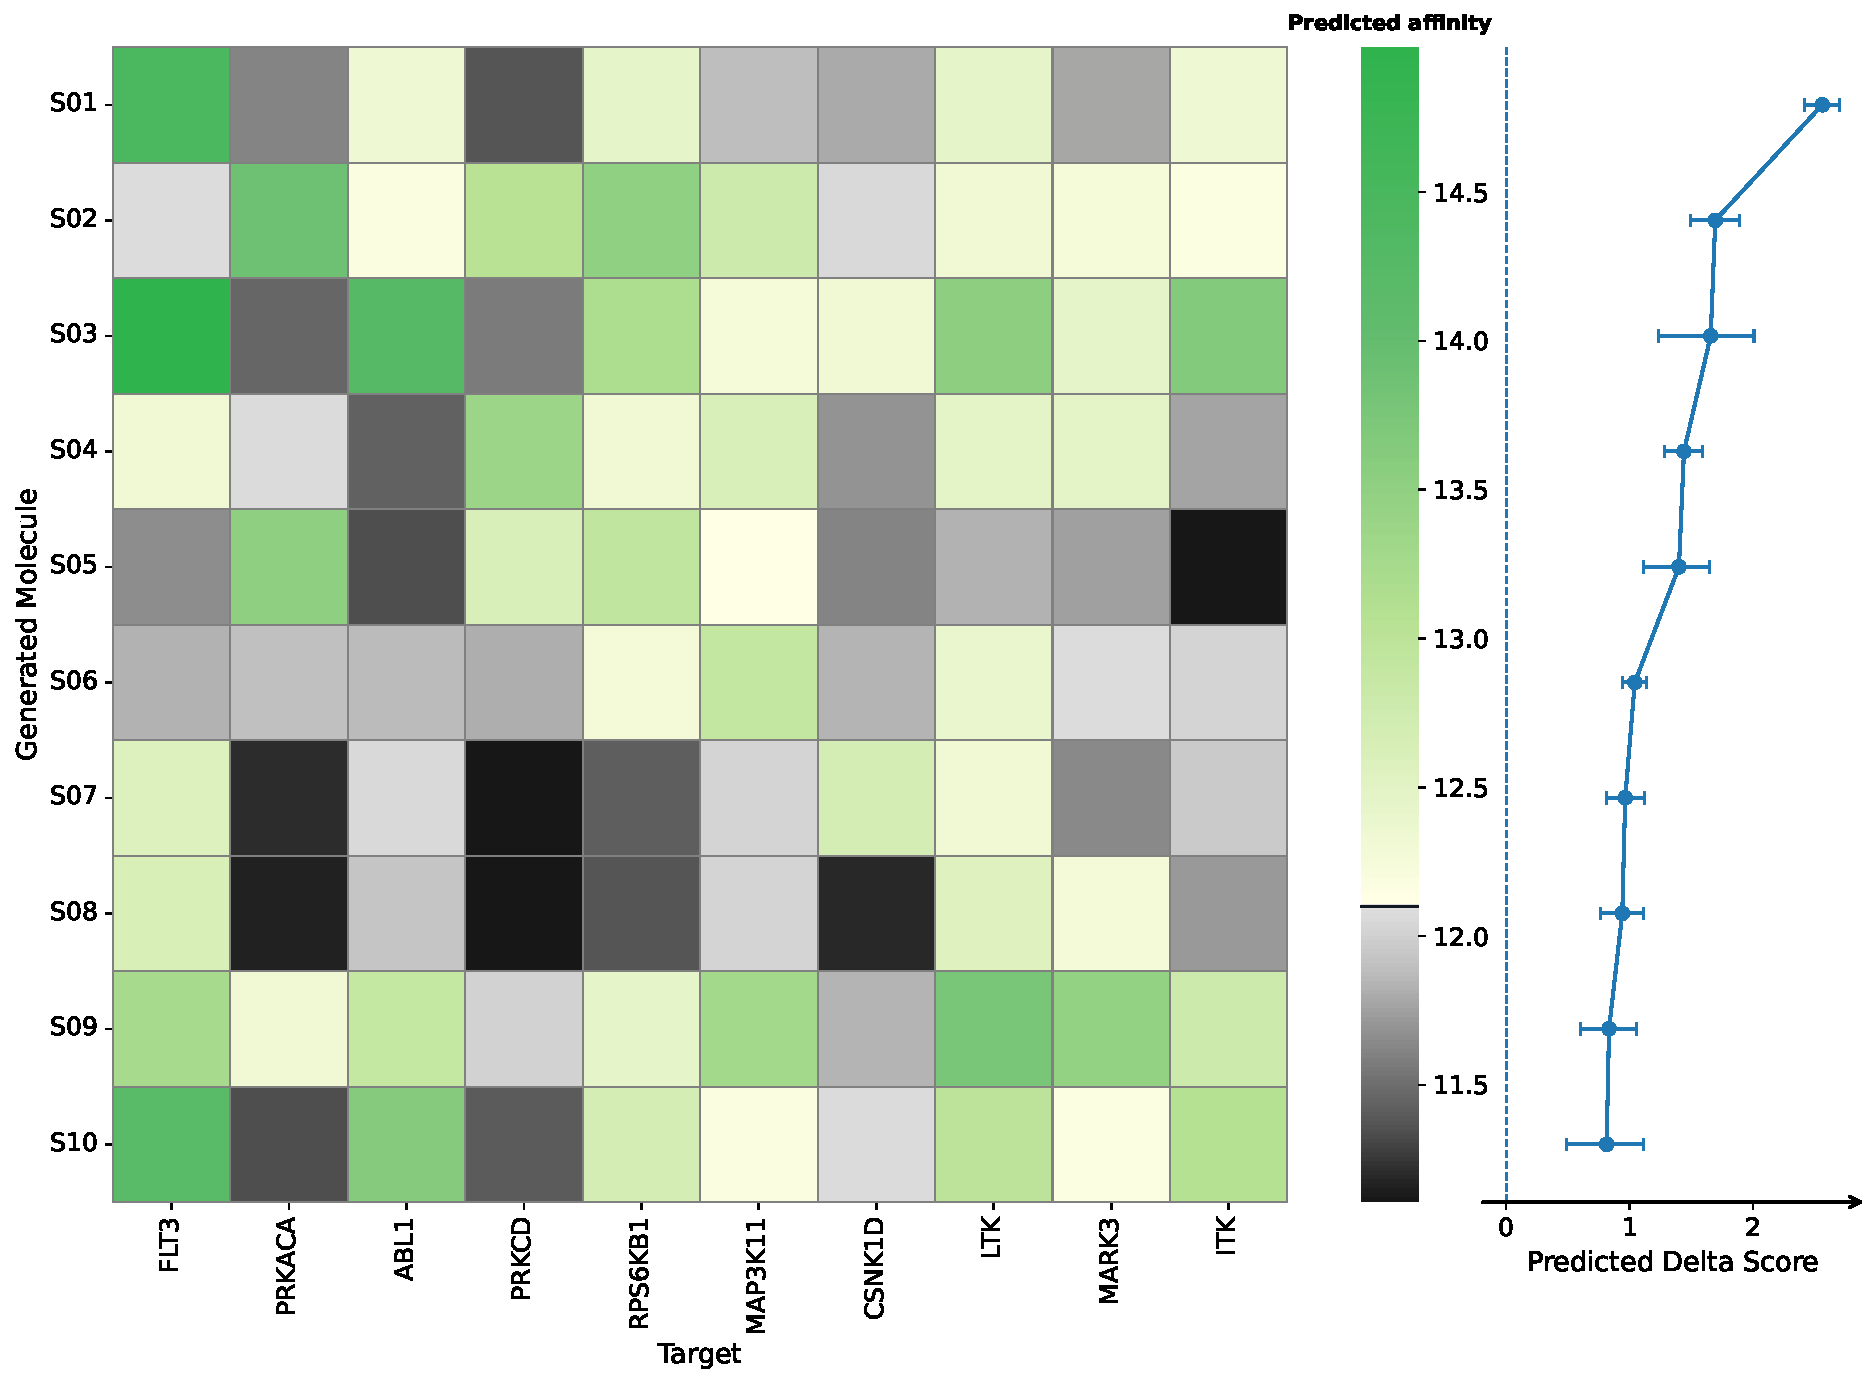
\includegraphics[width=\linewidth]{figs/e7/kiba/best_targets_SelVAEGen.pdf}
        \caption{SelVAEGen}\label{fig:e7_sel_selvaegen}
    \end{subfigure}
    \hfill
    \begin{subfigure}{0.49\linewidth}
        \centering
        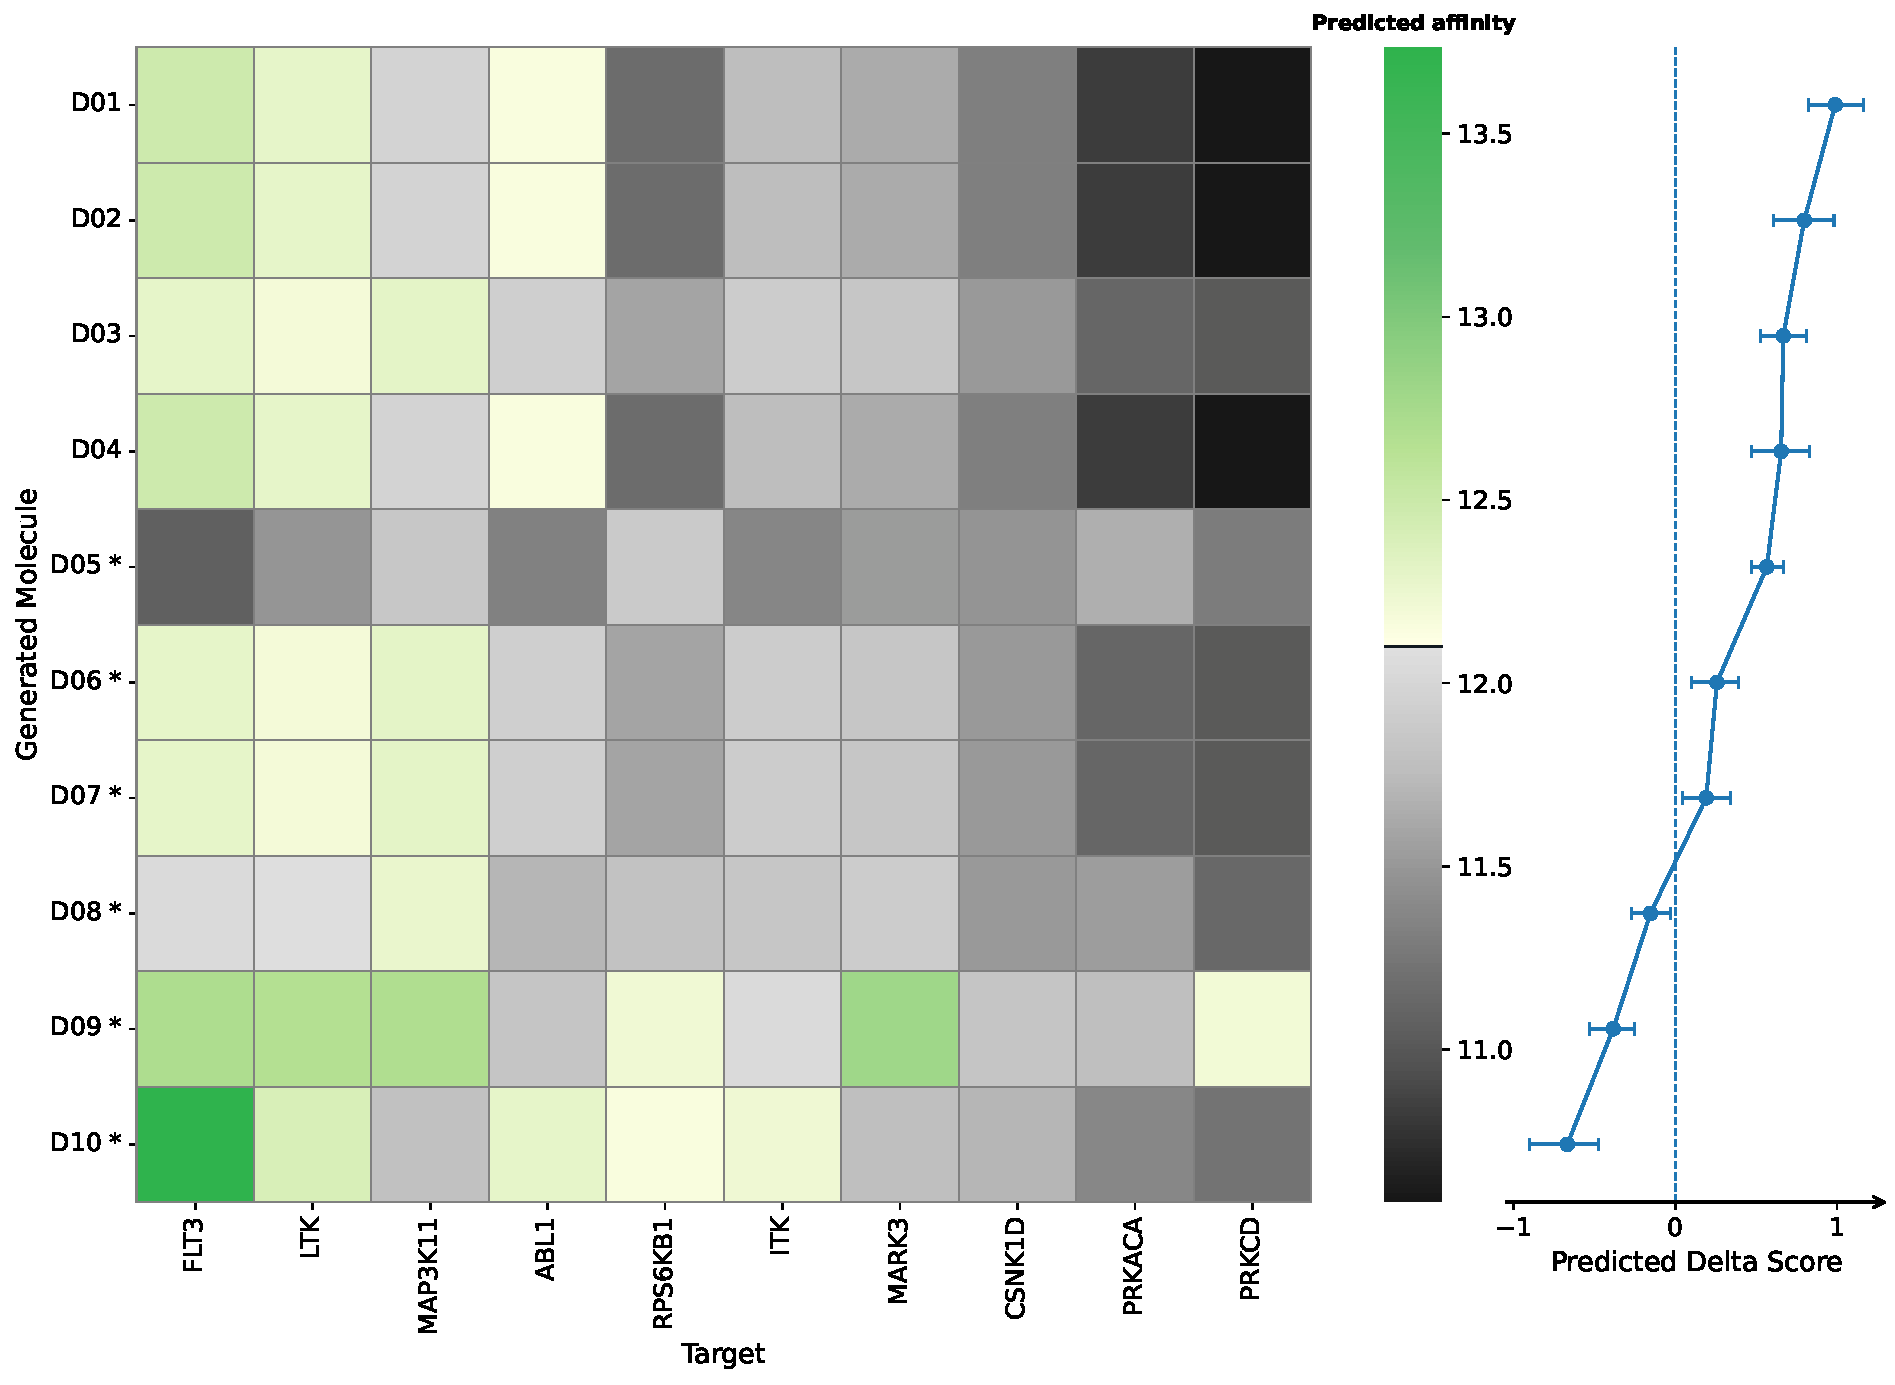
\includegraphics[width=\linewidth]{figs/e7/kiba/best_targets_DeepDTAGen.pdf}
        \caption{DeepDTAGen}\label{fig:e7_sel_deepdtagen}
    \end{subfigure}

    \begin{subfigure}{0.49\linewidth}
        \centering
        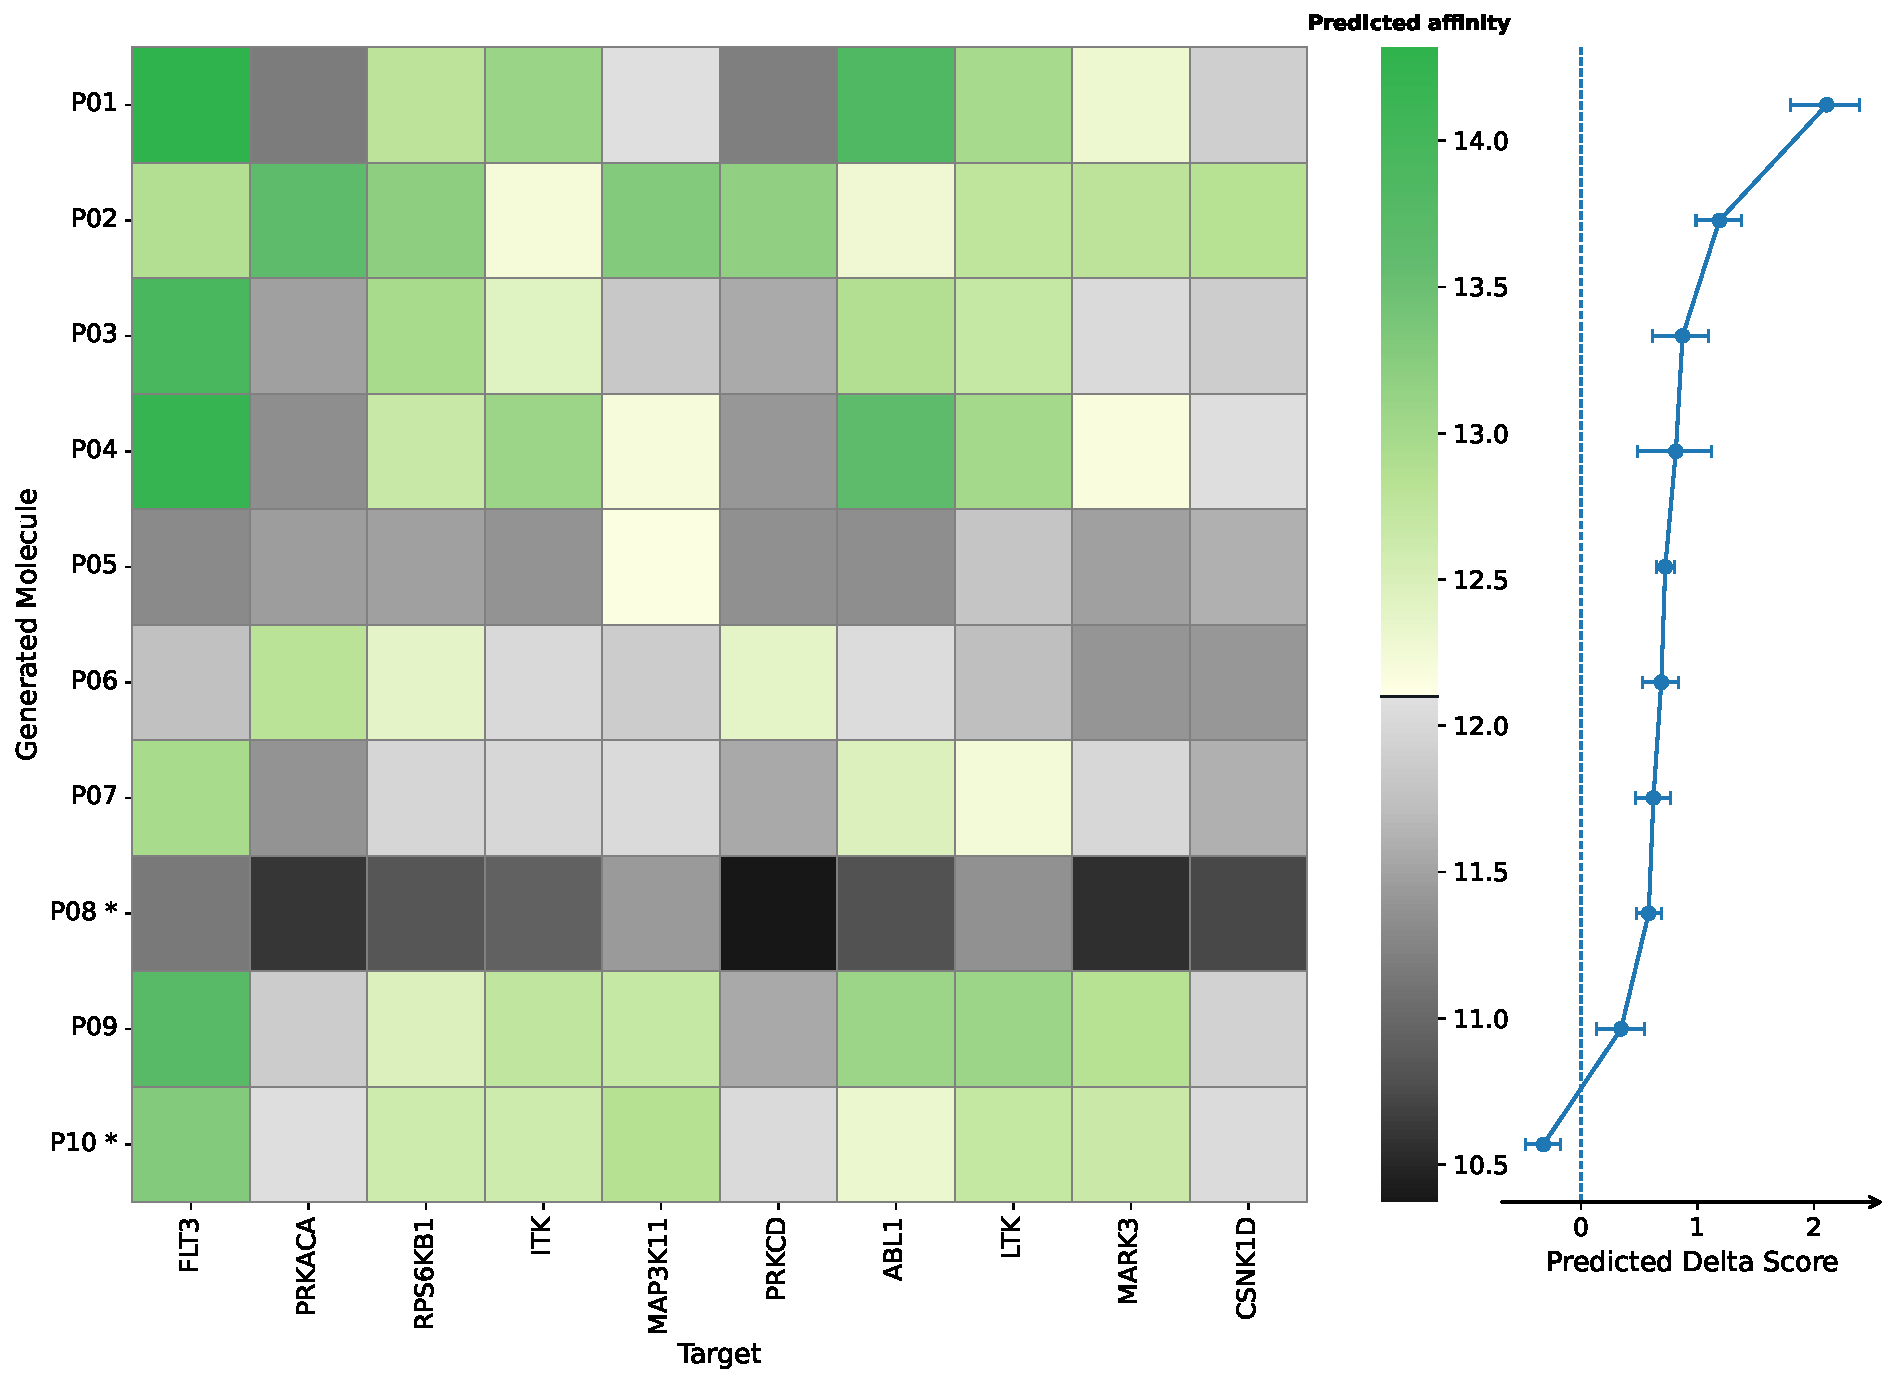
\includegraphics[width=\linewidth]{figs/e7/kiba/best_targets_Prot2Drug.pdf}
        \caption{Prot2Drug}\label{fig:e7_sel_prot2drug}
    \end{subfigure}
    \hfill
    \begin{subfigure}{0.49\linewidth}
        \centering
        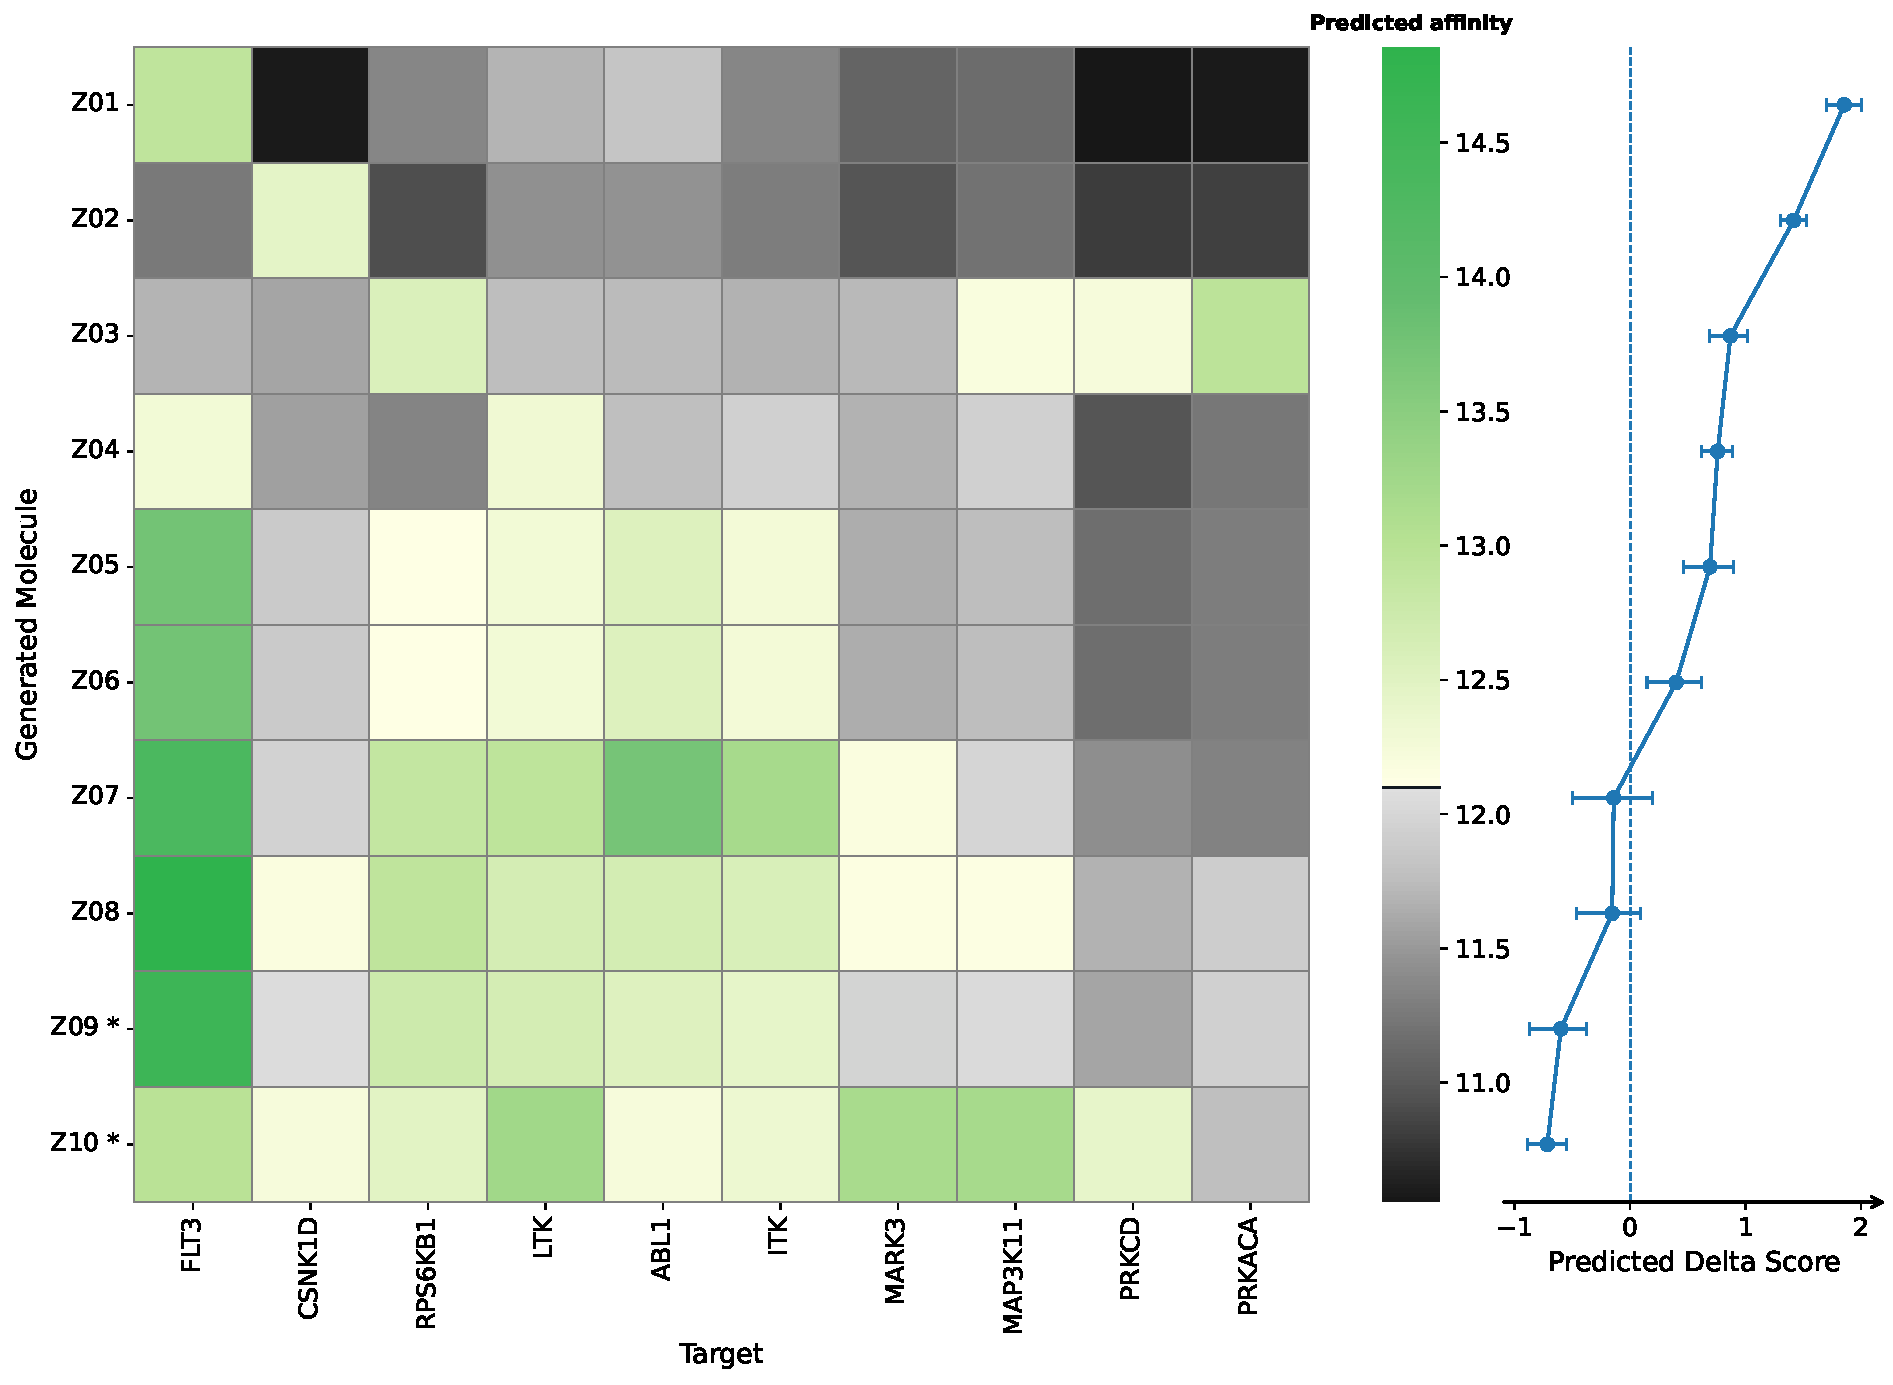
\includegraphics[width=\linewidth]{figs/e7/kiba/best_targets_ZeroGEN.pdf}
        \caption{ZeroGEN}\label{fig:e7_sel_zerogen}
    \end{subfigure}
    \caption[Most selective molecules in KIBA, by model.]{The most selective molecule generated for each of ten cold KIBA proteins by \textbf{(a)} SelVAEGen, \textbf{(b)} DeepDTAGen, \textbf{(c)} Prot2Drug and \textbf{(d)} ZeroGEN. Rows are selected molecules and columns are conditioning proteins, named by UniProt gene symbol. Diagonal cells give predicted affinity for the intended target. Off-diagonal cells give predicted affinity for an alternative. Gray cells are below the KIBA positive-affinity threshold of $12.1$. The strip on the right gives each molecule's $\delta$ score: its on-target prediction minus the mean prediction for the other nine proteins, with a percentile bootstrap $95\%$ confidence interval over that off-target panel. A strong green diagonal against darker off-diagonal cells indicates the desired target preference, most visible for SelVAEGen.}
    \label{fig:e7_selectivity}
\end{figure}

Table \ref{tab:selective_molecules} lists the selected SelVAEGen molecules, and Figure \ref{fig:e7_structures} shows their structures. The table brings together each candidate's intended target, predicted on-target affinity, individual $\delta$ score and similarity to its nearest KIBA training molecule. PubChem identifiers are reported where an exact InChIKey lookup matched a registered compound.

The comparison with training molecules helps describe the structural changes proposed by the generator. Several candidates are close to known training examples, while others have lower similarity. Four of the ten differ from a training molecule by a single edit. Reading these structural comparisons alongside predicted affinity and $\delta$ shows both the chemical relationship to the training set and the target preference used to select each candidate.

\begin{figure}[ht]
    \centering
    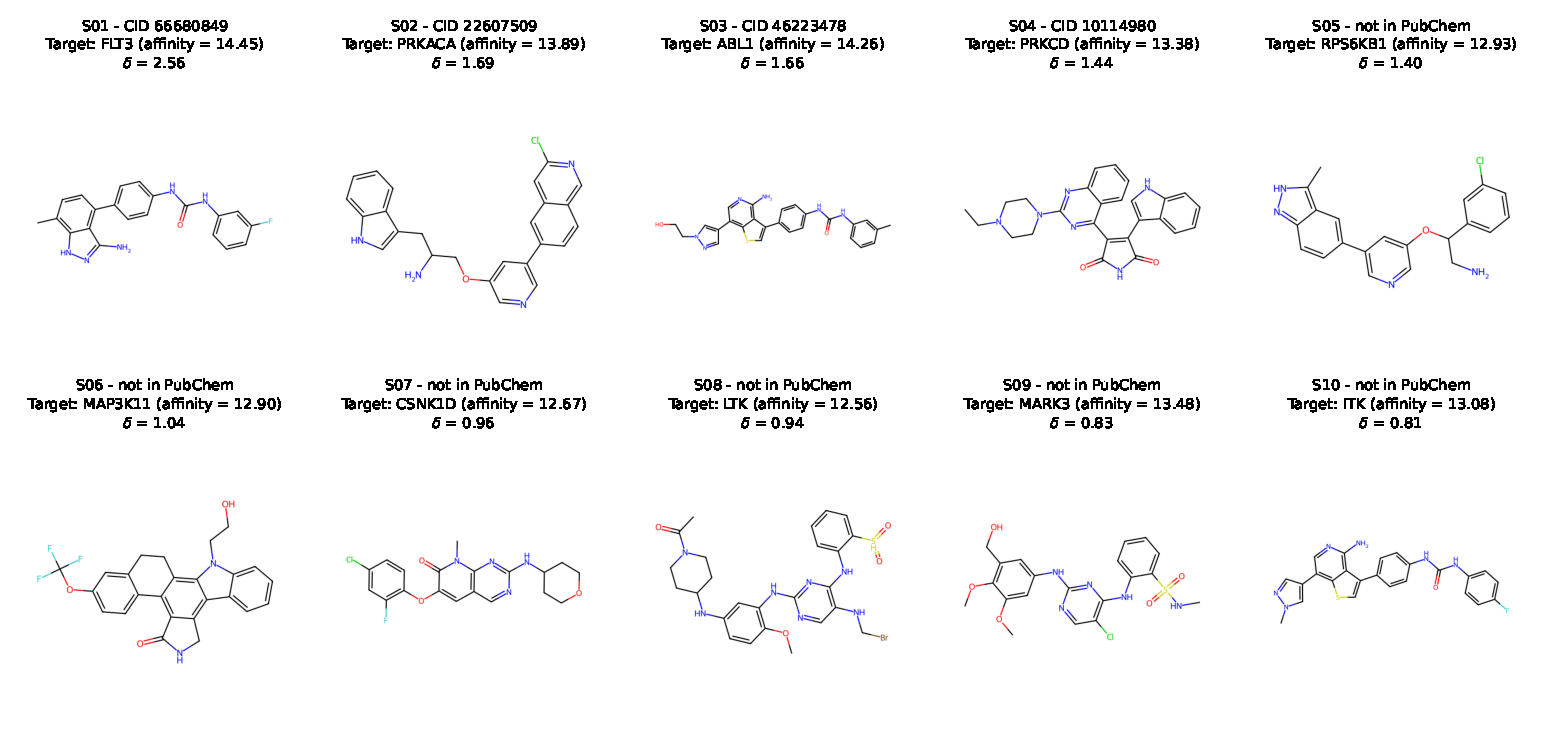
\includegraphics[width=\linewidth]{figs/e7/kiba/structures.pdf}
    \caption[Structures of the most selective molecules on KIBA.]{Structures of the ten
        most selective SelVAEGen molecules on KIBA. Each panel gives the PubChem identifier
        where the molecule matched a registered compound, the conditioning target with the
        predicted affinity against it, and the molecule's predicted $\delta$ score.}
    \label{fig:e7_structures}
\end{figure}

\begin{table}[H]
    \centering
    \caption[Most selective SelVAEGen molecules on KIBA.]{Most selective SelVAEGen molecules on KIBA, ordered by individual $\delta$ score. Target genes are named by their UniProt symbols. Affinity is the mean oracle prediction for the conditioning target, in KIBA score units, and Tanimoto similarity is measured against the nearest KIBA training molecule. PubChem identifiers are listed for the four molecules matched to registered compounds.}
    \label{tab:selective_molecules}
    \begin{tabular}{lcrlccc}
        \toprule
        \textbf{Molecule} & \textbf{PubChem ID} & \textbf{Target} & \textbf{Gene} & \textbf{Affinity} & \textbf{$\delta$} & \textbf{Tanimoto} \\
        \midrule
        S01 & 66680849 & 31 & FLT3 & 14.45 & 2.56 & 0.79 \\
        S02 & 22607509 & 7 & PRKACA & 13.89 & 1.69 & 0.82 \\
        S03 & 46223478 & 180 & ABL1 & 14.26 & 1.66 & 0.85 \\
        S04 & 10114980 & 130 & PRKCD & 13.38 & 1.44 & 0.80 \\
        S05 & - & 124 & RPS6KB1 & 12.93 & 1.40 & 0.63 \\
        S06 & - & 211 & MAP3K11 & 12.90 & 1.04 & 0.81 \\
        S07 & - & 123 & CSNK1D & 12.67 & 0.96 & 0.84 \\
        S08 & - & 195 & LTK & 12.56 & 0.94 & 0.46 \\
        S09 & - & 77 & MARK3 & 13.48 & 0.83 & 0.84 \\
        S10 & - & 115 & ITK & 13.08 & 0.81 & 0.84 \\
        \bottomrule
    \end{tabular}
\end{table}

Taken together, these qualitative examples show at the level of individual molecules what the
aggregate metrics report: the generated structures resemble drug-like chemistry, their
predicted affinities sit above those measured for the same proteins, and the molecules made
for one protein form recognizable structural groups.

\FloatBarrier
\subsection{Ablation studies}\label{sec:temp}
The comparisons above evaluate the final model. We now examine which design choices contribute to its performance and how generation changes when the trained model is sampled under different conditions. The appendix reports the comparison of encoder and decoder branches.

\subsubsection{Molecular string notation}\label{sec:notation}

The molecular string notation affects how easily a decoder can produce a valid structure. We compare SMILES and SELFIES using both validity and Effective $\Delta$, so that a gain in valid output can be considered alongside its contribution to selective generation. Paired Student's $t$-tests compare runs with matching random seeds, and the two resulting $p$-values are corrected using the BH procedure. Table \ref{tab:e3_tests} reports the results.

\begin{table}[ht]
    \centering
    \caption[SMILES and SELFIES on KIBA.]{Comparison of SMILES and SELFIES on KIBA. Difference is SELFIES minus SMILES. The paired Student's $t$-tests compare matching random seeds, and $p_{\mathrm{BH}}$ gives the Benjamini-Hochberg-corrected value. SELFIES improves validity, while the experiment detects no significant difference in Effective $\Delta$.}
    \label{tab:e3_tests}
    \begin{tabular}{lcccccc}
        \toprule
        \textbf{Metric} & \textbf{SMILES} & \textbf{SELFIES} & \textbf{Difference} & \textbf{$t$} & \textbf{$p_{\mathrm{BH}}$} \\
        \midrule
        Effective $\Delta$ & $0.1078 \pm 0.0272$ & $0.1067 \pm 0.0219$ & $-0.0011$  & $-0.2140$ & 0.8410 \\
        Validity & $0.9243 \pm 0.0207$ & $1.0000 \pm 0.0000$ & $+0.0757$ & $8.1641$ & 0.0025 \\
        \bottomrule
    \end{tabular}
\end{table}

SELFIES achieved validity $1.0000$ in every run, compared with $0.9243 \pm 0.0207$ for SMILES. The average difference is $7.57$ percentage points and remains statistically significant after correction ($p_{\mathrm{BH}}=0.0025$). No statistically significant difference in Effective $\Delta$ was detected ($p_{\mathrm{BH}}=0.8410$). SELFIES therefore provides more reliable structural validity, while the experiment does not establish a corresponding improvement in the combined measure of selectivity and generation quality.

\subsubsection{Loss function}
The loss comparison asks whether the affinity ranking loss $\mathcal{L}_{\mathrm{aff}}$, selectivity ranking loss $\mathcal{L}_{\mathrm{sel}}$, and distributional selectivity loss $\mathcal{L}_{\mathrm{dist}}$ improve generation. Every configuration retains the reconstruction loss and prior regularization loss. ``None'' in Table \ref{tab:e4_losses} denotes this common control without the three additional losses. We compare each configuration with that common control using Dunnett's multiple comparison procedure \parencite{dunnett1955multiple}. Table \ref{tab:e4_losses} reports Effective $\Delta$, its difference from the control and the adjusted $p$-value for each comparison.

\begin{table}[H]
    \centering
    \caption[Comparison of training objectives on KIBA.]{Comparison of additional training losses on KIBA. Every configuration retains the reconstruction loss and prior regularization loss. The additional terms are the affinity ranking loss $\mathcal{L}_{\mathrm{aff}}$, selectivity ranking loss $\mathcal{L}_{\mathrm{sel}}$, and distributional selectivity loss $\mathcal{L}_{\mathrm{dist}}$. ``None'' denotes the common control. Differences are relative to this control, with $p$-values adjusted using Dunnett's multiple comparison procedure.}
    \label{tab:e4_losses}
    \begin{tabular}{lccc}
        \toprule
        \textbf{Additional losses} &
        \textbf{Effective $\Delta$} &
        \textbf{Difference} &
        \textbf{$p$} \\
        \midrule
        None
        & $0.0831 \pm 0.0185$
        & -
        & - \\
        $\mathcal{L}_{\mathrm{dist}}$
        & $0.0949 \pm 0.0327$
        & $+0.0118 \pm 0.0159$
        & 0.1132 \\
        $\mathcal{L}_{\mathrm{aff}} + \mathcal{L}_{\mathrm{sel}}$
        & $0.1148 \pm 0.0320$
        & $+0.0317 \pm 0.0154$
        & 0.0003 \\
        $\mathcal{L}_{\mathrm{aff}} + \mathcal{L}_{\mathrm{sel}} + \mathcal{L}_{\mathrm{dist}}$
        & $0.1156 \pm 0.0303$
        & $+0.0325 \pm 0.0163$
        & 0.0003 \\
        \bottomrule
    \end{tabular}
\end{table}

Both configurations containing the affinity ranking and selectivity ranking losses significantly outperform the control. Their mean Effective $\Delta$ values are nearly identical, whether or not the distributional selectivity loss is included. The distributional selectivity loss alone gives a smaller mean increase of $+0.0118$, which is not statistically significant in this comparison. The evidence therefore supports the contribution of the affinity ranking and selectivity ranking losses together.

\subsubsection{Sampling temperature}
Sampling temperature changes which tokens the trained decoder is likely to choose. A lower temperature concentrates probability on the most likely tokens, and a higher temperature gives less likely alternatives a greater chance of being selected \parencite{caccia2020language}. This provides a way to change the diversity of generated molecules without retraining the model.

For each independent SelVAEGen training seed on KIBA, we generate molecules at temperatures from $0$ to $5$ in steps of $0.25$. Figure \ref{fig:qual_e8} reports generation quality, Figure \ref{fig:chem_e8} reports affinity and chemical properties, and Figure \ref{fig:sel_e8} reports selectivity.

Validity remains at one throughout the range, while uniqueness and novelty rise with temperature. At higher temperatures, however, predicted affinity, QED and selectivity decrease, while SA and FCD increase. Directional Consistency approaches its chance reference of $0.5$, and the Tanimoto Gap approaches zero. The model explores more structures, but those structures show less dependence on the intended protein.

Effective $\Delta$ reaches a maximum at an intermediate temperature. Initially, greater uniqueness allows more generation attempts to contribute to the score. Beyond that region, the loss of selectivity outweighs the gain in diversity. Temperature therefore provides a practical means of adjusting the balance between the variety of a generated library and its predicted target preference.

\begin{figure}[H]
    \centering
    
\includegraphics[width=\linewidth]{figs/e8/seq_quality.pdf}
    \caption[Generation metrics across sampling temperatures on KIBA.]{Validity, uniqueness and novelty as a function of SelVAEGen's sampling temperature on KIBA. Validity remains stable while uniqueness and novelty increase with temperature. Shaded bands are 95\% confidence intervals of the mean over seeds. The gray dotted line marks the reference temperature $T=1$, used in the other experiments.}
    \label{fig:qual_e8}
\end{figure}

\begin{figure}[H]
    \centering
    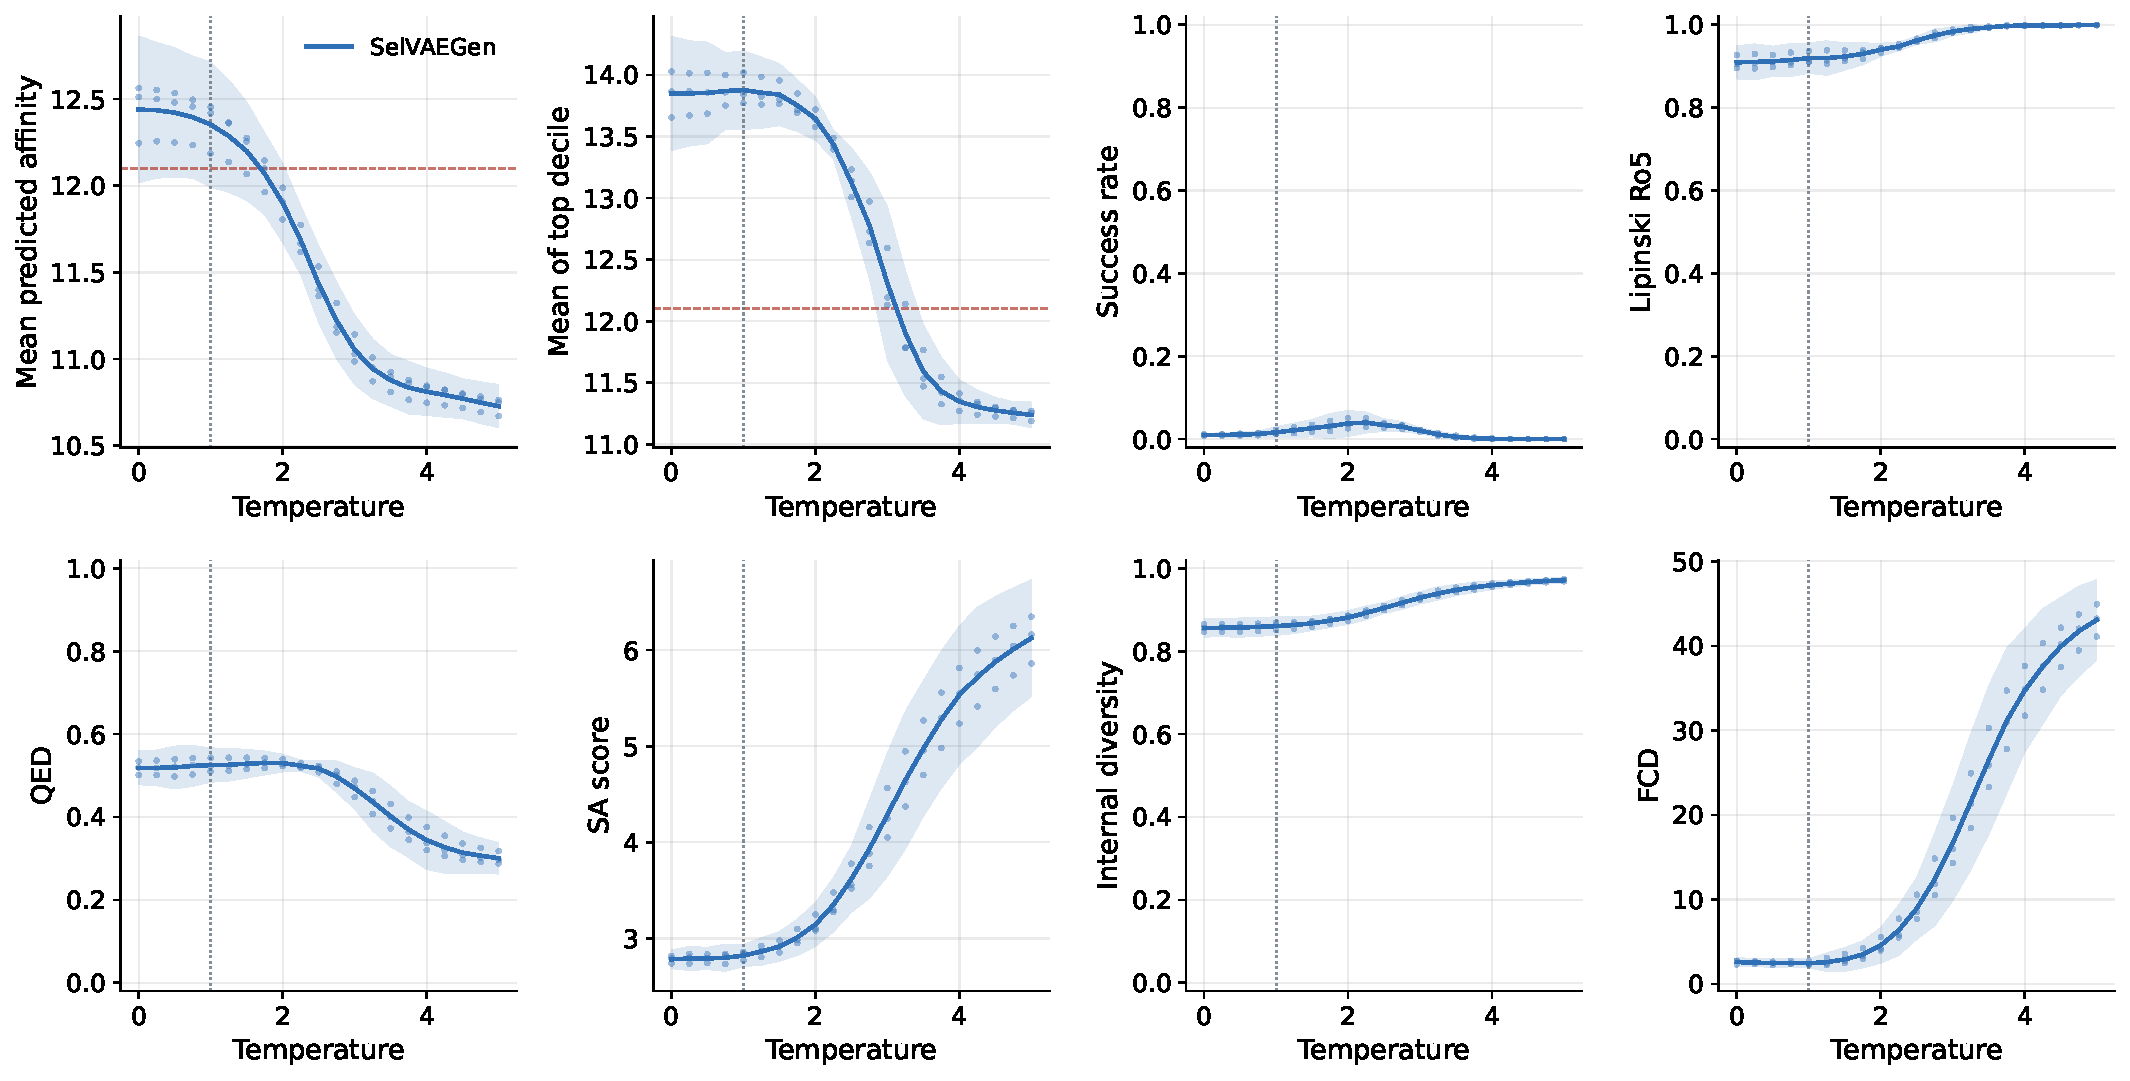
\includegraphics[width=\linewidth]{figs/e8/seq_potency_chemistry.pdf}
    \caption[Chemical metrics across sampling temperatures on KIBA.]{Predicted affinity and chemical properties as a function of SelVAEGen's sampling temperature on KIBA. Higher temperatures reduce predicted affinity and QED while increasing synthetic accessibility scores and FCD. The red dashed line marks the dataset's positive-affinity threshold. Shaded bands are 95\% confidence intervals of the mean over seeds, and the gray dotted line marks the reference temperature $T=1$, used in the other experiments.}
    \label{fig:chem_e8}
\end{figure}

\begin{figure}[H]
    \centering
    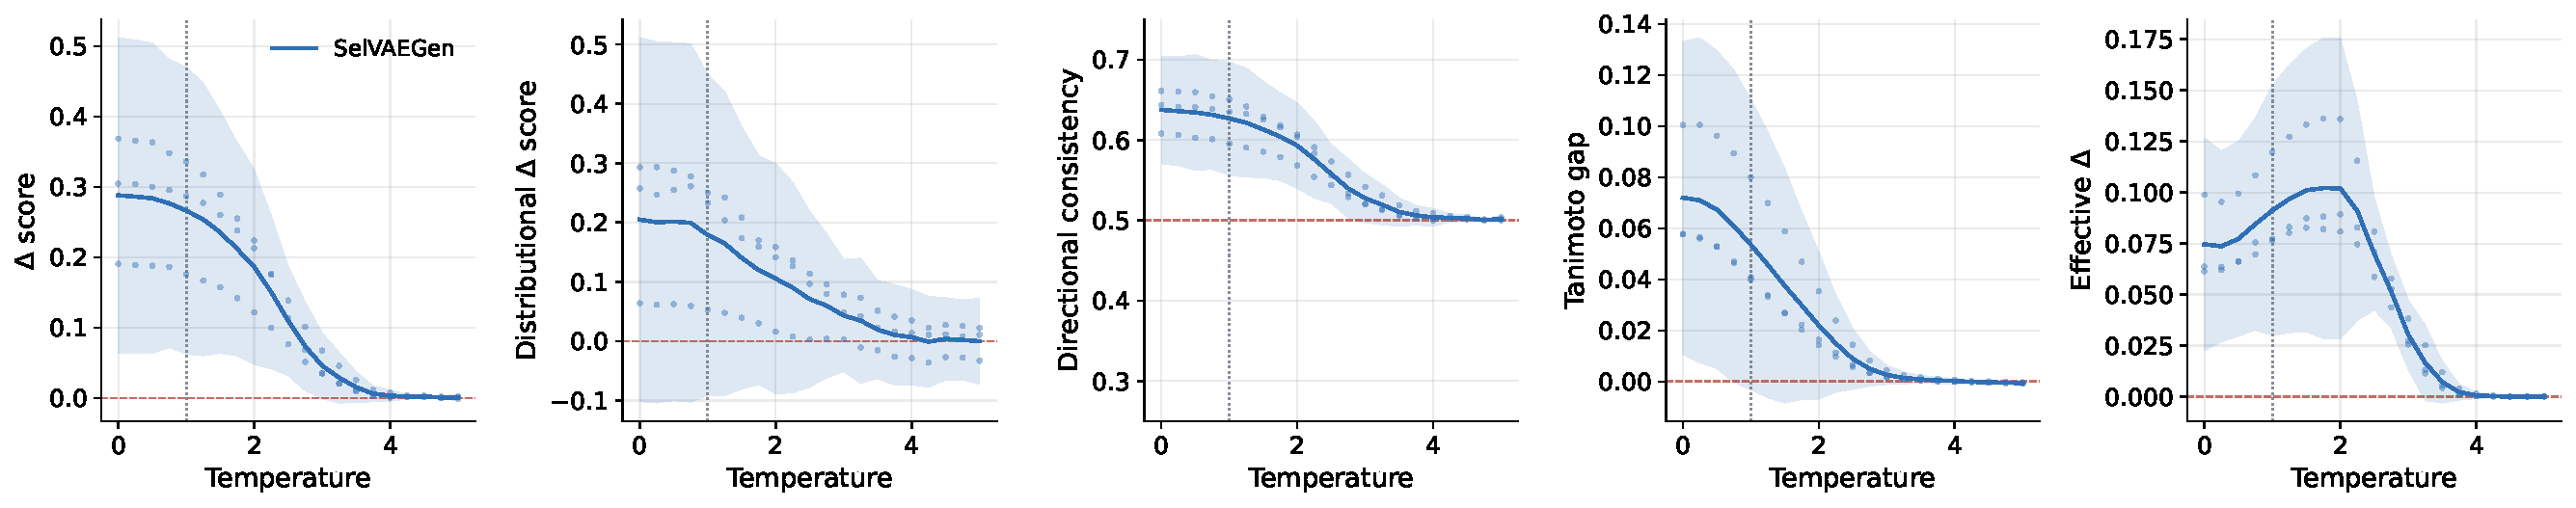
\includegraphics[width=\linewidth]{figs/e8/seq_selectivity.pdf}
    \caption[Selectivity metrics across sampling temperatures on KIBA.]{Selectivity metrics as a function of SelVAEGen's sampling temperature on KIBA. Increasing temperature reduces target preference, while Effective $\Delta$ reaches its maximum at an intermediate temperature. Red dashed lines mark the reference values for a non-selective model. Shaded bands are 95\% confidence intervals of the mean over seeds, and the gray dotted line marks the reference temperature $T=1$, used in the other experiments.}
    \label{fig:sel_e8}
\end{figure}

\subsubsection{Protein similarity}

A protein may be absent from the training set while remaining highly similar to proteins seen during training. We therefore ask whether SelVAEGen performs better on test targets that are more familiar in sequence space. Each test protein is compared with all training proteins using local sequence alignment with the standard BLASTp scoring scheme \parencite{Altschul1997Gapped}. Target familiarity is defined by the smallest E-value obtained against any training protein. Because E-values span many orders of magnitude, we report similarity as $-\log_{10}E$, so that larger values indicate a closer training sequence, and cap values at 300 when numerical underflow occurs.
Test proteins are ordered by this similarity and divided into four equally sized groups. Three selectivity metrics are then recomputed within each group. Figure \ref{fig:e9} shows the resulting $\Delta$, Directional Consistency and Effective $\Delta$ scores, together with performance on the training proteins as a reference. Across datasets, the quartiles cover a broad range of sequence familiarity: intra-group mean $-\log_{10}E$ ranges from 58 to 273 on KIBA, 54 to 295 on Davis, 10 to 272 on BindingDB and 9 to 229 on Papyrus.

Despite this range, selectivity does not show a consistent relationship with proximity to the training proteins. For each seed, we fit the value of each selectivity metric as a function of $-\log_{10}E$ and test the resulting slopes against zero across seeds. After correcting the twelve tests jointly for multiple comparisons, eleven show no significant association. The only exception is $\Delta$ on Davis, with an adjusted $p=0.031$ and a positive slope of $0.005$ per unit of $-\log_{10}E$. This effect is not reproduced by the other selectivity metrics or datasets, however, and the uncertainty intervals of the four Davis groups overlap substantially.
This experiments provides no evidence of a systematic deterioration in selectivity as test proteins become more distant from the training set.

\begin{figure}[H]
    \centering
    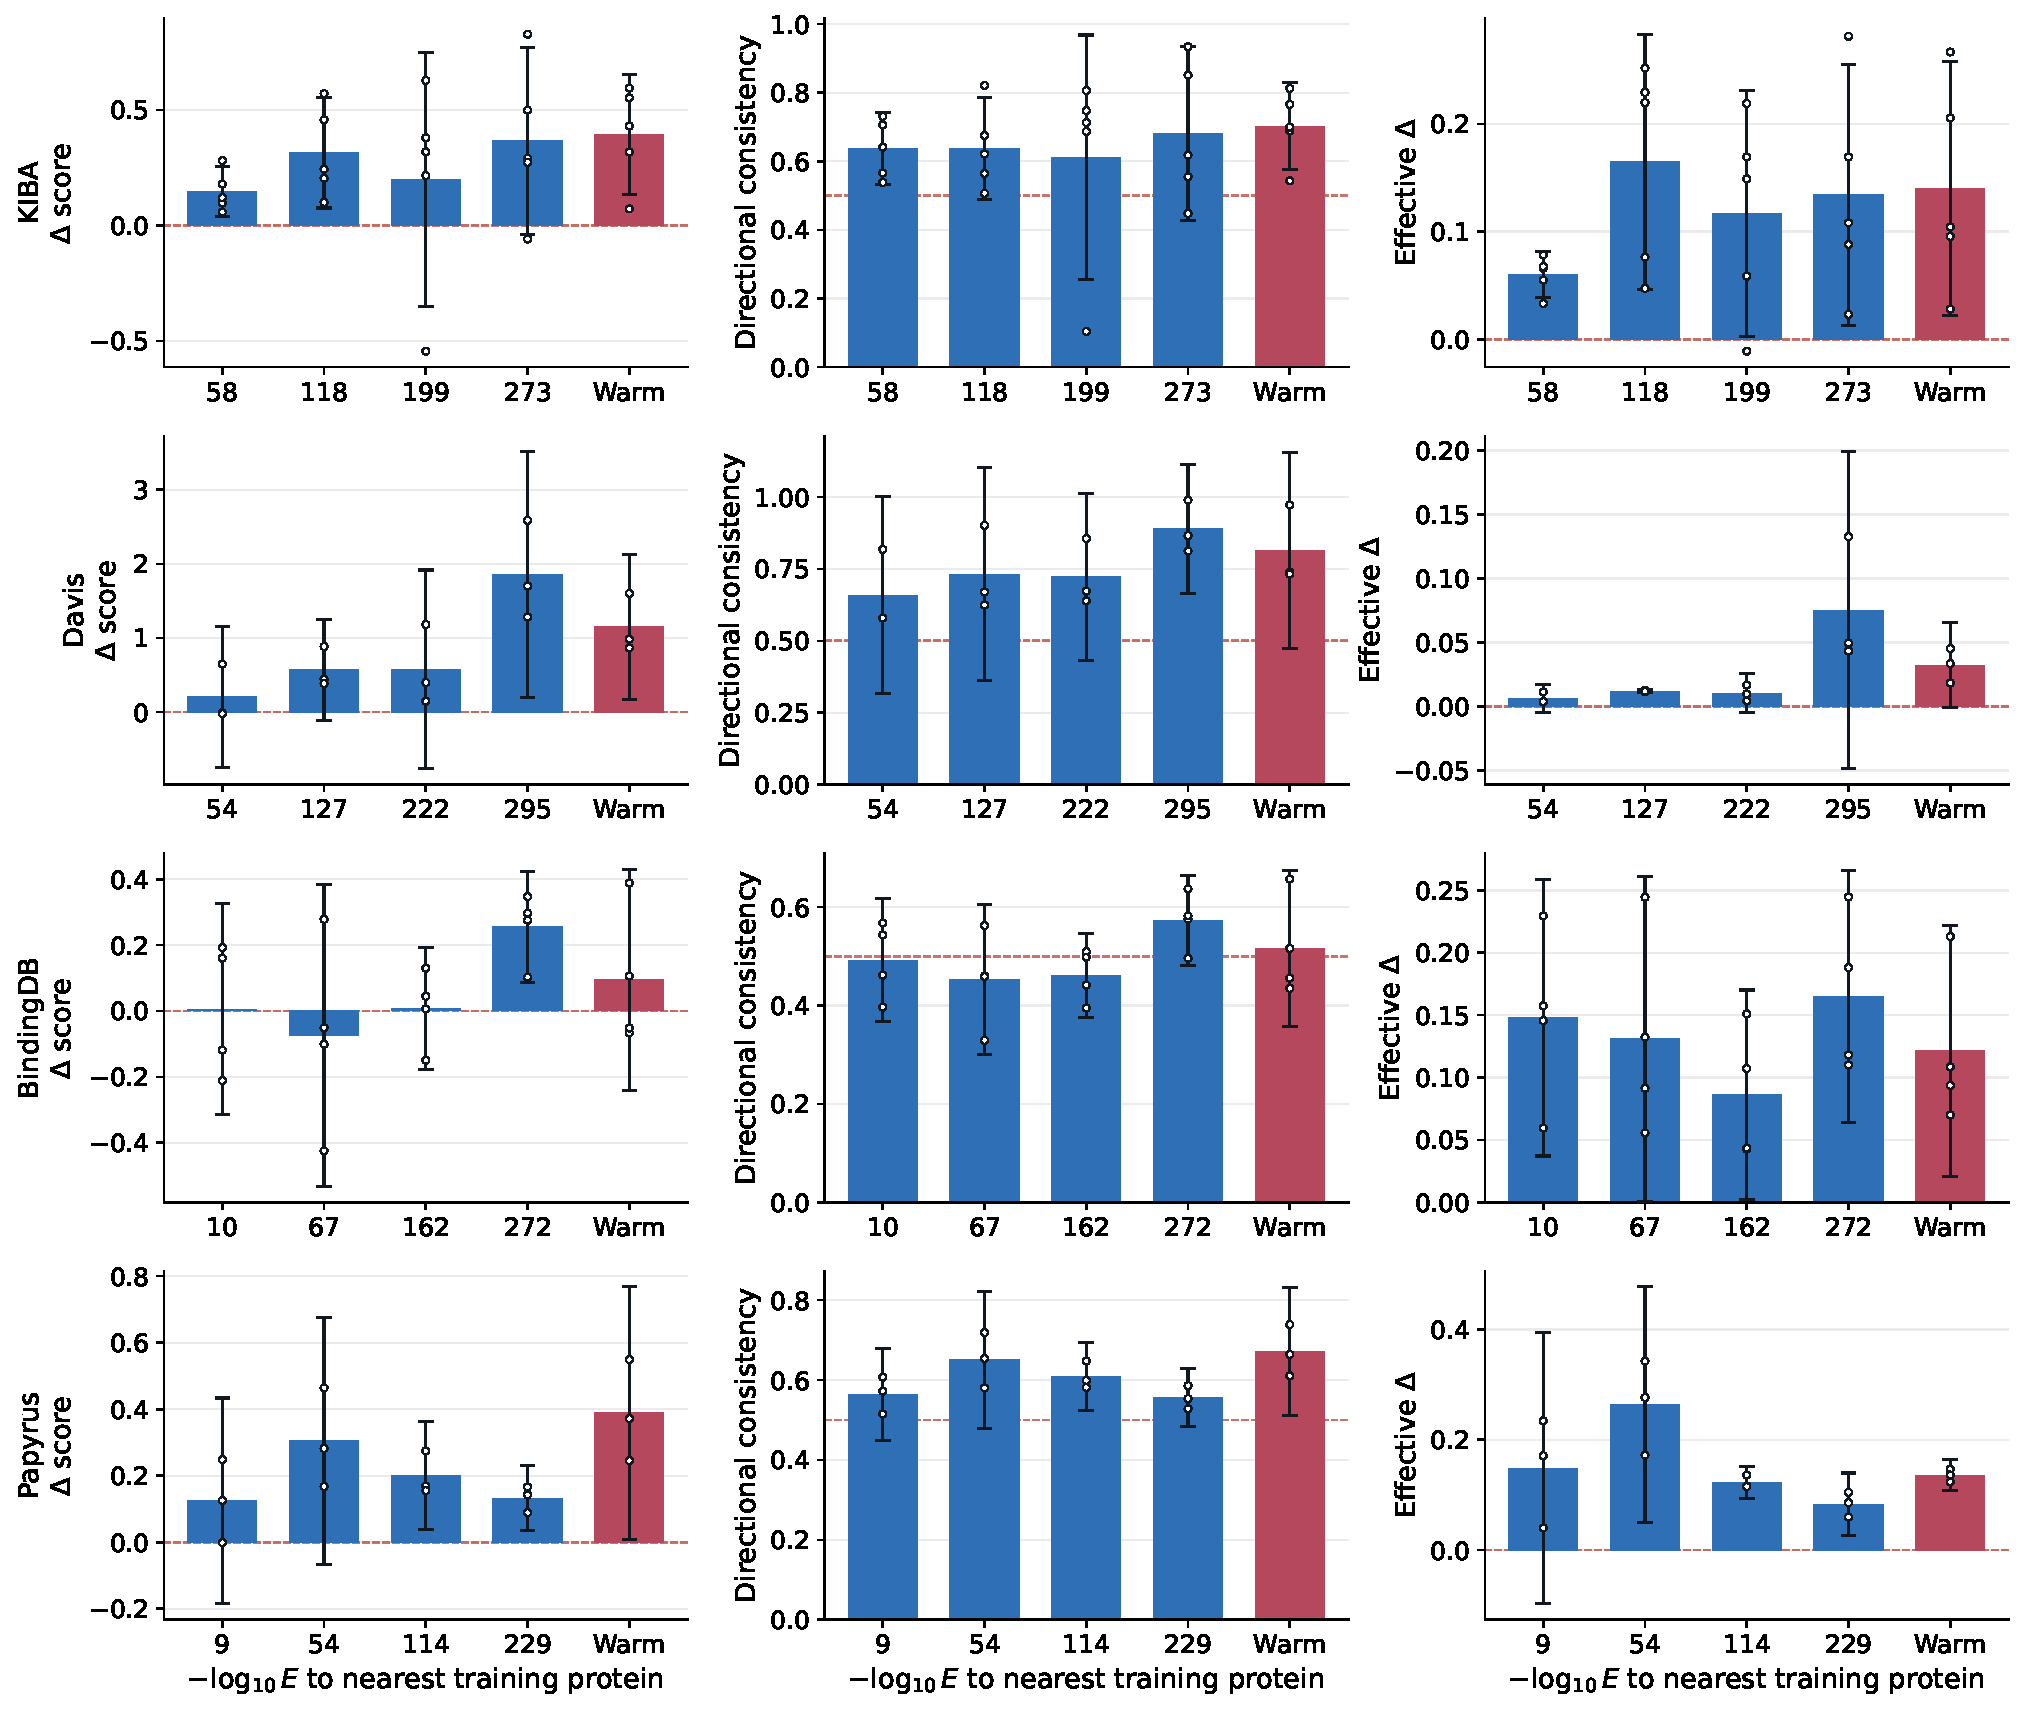
\includegraphics[width=\linewidth]{figs/e9/similarity_grid_evalue.pdf}

    \caption[Selectivity against target familiarity.]{
        Selectivity as a function of target familiarity. Rows correspond to datasets and columns to the three selectivity metrics. Each test protein is matched to its closest training protein according to the E-value of their local sequence alignment and assigned to one of four familiarity groups. Blue bars show the mean metric within each group and are labeled by the corresponding intra-group mean $-\log_{10}E$, with larger values indicating greater similarity to the training set. Red bars show the same metric on training proteins. Error bars denote $95\%$ confidence intervals over seeds and open circles show individual seeds. The dashed line indicates the value expected from a generator that ignores its conditioning protein. Groups are ordered from the least to the most familiar targets.
    }
    \label{fig:e9}
\end{figure}

\subsection{Discussion}

Affinity and selectivity are distinct properties of protein-targeted generation. The competing models obtain favorable predicted on-target affinities, yet their Directional Consistency remains close to chance, showing that high affinity towards the conditioning protein does not imply preference for that protein over alternatives. SelVAEGen instead shows a consistent target-dependent advantage across the proposed selectivity metrics.

This difference is consistent with the information provided during training. Reconstructing molecules associated with a protein does not penalize those molecules for also being compatible with other proteins. SelVAEGen introduces this comparison explicitly: its ranking objectives organize molecules relative to protein representations, and the selectivity-ranking loss directly compares two proteins for the same molecule. The ablations support the contribution of the ranking losses.

The results also show that dataset density matters more than dataset size alone. The strongest improvements occur on KIBA and Davis, where molecules are measured against several proteins. In BindingDB and Papyrus, most molecules provide few or no direct cross-protein comparisons. Learning selective generation depends strongly on measurements that compare the same drugs across several targets.

These conclusions remain limited to predicted selectivity. The oracles recover affinity orderings imperfectly, and their disagreement increases for less familiar molecules.

When considering less familiar held-out proteins, no dependence on target similarity is detectable. Raising SelVAEGen's sampling temperature can trade some target preference for uniqueness, novelty and chemical quality. It also retains the highest Effective $\Delta$, and its utility is significantly positive across all four datasets. Together, these results support the central the idea that explicitly training a generator from relative affinity information can improve its predicted preference for the protein supplied as a condition.

\newpage
\chapteropeninginline
{Conclusion}

This dissertation investigated whether protein-targeted molecular generators produce molecules that preferentially bind to the proteins for which they were generated. The results show that high predicted on-target affinity alone does not establish this property: several competing generators perform well under conventional affinity evaluation while showing little preference for their conditioning targets.

To address this, we introduced a framework for evaluating selective generation and proposed SelVAEGen, which uses relative affinity information to organize proteins and molecules in a shared latent space. Across four standard benchmark datasets, SelVAEGen shows stronger predicted selectivity than the competing methods and is the only model with significantly positive utility on all four datasets after correction for multiple comparisons.

Thus, protein-targeted generation should be evaluated by comparing each generated molecule against both its intended target and alternative proteins. Incorporating the same relative information during training provides a direct way to improve this target preference.

\subsection{Limitations and future work}\label{sec:limitations}

The main limitation is that the reported selectivity is predicted rather than experimentally measured. Although several affinity models are used and their behavior is evaluated on held-out data, their predictions remain approximations. Docking, molecular dynamics and experimental affinity measurements would provide validation of whether the observed target preferences correspond to biological selectivity.

A second limitation is data sparsity. Selectivity requires measurements of the same molecule against several proteins, yet such comparisons are rare in large affinity datasets. Future datasets with broader and more systematic cross-target measurements would therefore be especially valuable. Further work should also address the observed trade-off between selectivity, diversity and chemical quality, and extend the framework from whole-protein conditioning to particular binding pockets or protein interfaces.

\subsection{Data availability and reproducibility}
The entirety of the data and code used to conduct all experiments is available on \href{https://github.com/DutraIRS/SelVAEGen}{GitHub}. Datasets used in this work are publicly available, and the source can be found on their original publications' repositories. All experiments were conducted on a NVIDIA A100 80 GB GPU, and one complete training run of SelVAEGen takes around one hour.

\newpage
\phantomsection
\addcontentsline{toc}{section}{Appendix}
\section*{Appendix}
\setcounter{figure}{0}
\setcounter{table}{0}
\renewcommand{\thefigure}{S\arabic{figure}}
\renewcommand{\thetable}{S\arabic{table}}
This section presents the alternative architectures considered when developing SelVAEGen. The comparison asks whether reading a molecule as a graph, either alone or alongside its string representation, improves generation, and whether the latent representation is better decoded into a string or directly into a graph. We first introduce the representations and their motivation, then describe the alternatives and compare their results.

\subsubsection*{Graph-based representation}
A molecule can be represented as a graph $\Gcal=(\Vcal,\Ecal)$: each node is an atom, with features such as element, charge and hybridization, and each edge is a bond, with an associated bond order, such as single, double or triple. Graph neural networks process this structure through message passing \parencite{Gilmer_Schoenholz_Riley_Vinyals_Dahl_2017}. At each layer, an atom receives information from its neighbors and uses it to update its representation:
\begin{equation*}\label{eq:mpnn}
    h_v^{(\ell+1)} = \UPD\!\left(h_v^{(\ell)},\ \AGG_{u\in\mathcal{N}(v)}\MSG\!\left(h_v^{(\ell)},h_u^{(\ell)},e_{uv}\right)\right),
\end{equation*}
where $\MSG$ forms a message along each edge, $\AGG$ combines the messages from the neighborhood $\mathcal{N}(v)$ without depending on their order, and $\UPD$ combines this information with the atom's previous state. A $\READOUT$ over all nodes then produces a representation of the complete molecule. Different graph neural networks make different choices for these operations. Graph convolutional networks \parencite{Kipf_Welling_2017} use a degree-normalized sum, graph isomorphism networks \parencite{Xu_Hu_Leskovec_Jegelka_2019} use a sum followed by an MLP, and graph attention networks \parencite{Velickovic_Cucurull_Casanova_Romero_Lio_Bengio_2018} learn how much weight to assign to each neighbor.

Encoding starts from a graph whose atoms and bonds are already known. Decoding must instead construct them, while also dealing with the absence of a canonical node ordering. GraphVAE \parencite{Simonovsky_Komodakis_2018} predicts a dense probabilistic adjacency matrix in a single step and uses approximate graph matching to compare it with the target graph, an operation that is expensive and scales poorly. JT-VAE \parencite{Jin_Barzilay_Jaakkola_2018} generates a junction tree of chemically valid fragments and then assembles them. This guarantees validity, but restricts generation to a fixed vocabulary of substructures.

\subsubsection*{Multi-view representation}
A graph and a string describe the same molecule, but make different information directly available to the model. In a graph, atoms that share a bond are neighbors, so connectivity is explicit. Relating distant atoms, however, requires information to pass through several layers. In a string, self-attention can connect any two positions in one step, but the model must learn how punctuation and ring-closure digits encode connectivity. A fingerprint provides another view: a fixed vector summarizing the presence of substructures, which may leave out information needed to distinguish molecules.

The motivation for combining these views is that information which is difficult to extract from one may be easier to obtain from another. A combined representation might therefore be more useful than any individual view. \textcite{Zhu_Xia_Wu_Xie_Zhou_Qin_Li_Liu_2023} tested this idea by jointly pre-training a Transformer on SMILES strings and a GNN on molecular graphs. Each view was required to predict masked content from the other, encouraging the encoders to learn from information beyond that most directly exposed by their own inputs. Their combined representations outperformed equivalent single-view models on downstream property prediction. Here, the architectural comparison tests whether combining views also helps the selective generation task.

\paragraph{Graph decoder.}
The alternative graph decoder expands the latent representation into a fixed number of learned node queries and processes them through four Transformer layers. Each query provides a position for a possible atom in the output graph. As in the sequence decoder, protein-dependent affine transformations modulate the hidden states.

The decoder first predicts whether each possible node exists. For the nodes that exist, it predicts categorical distributions over atom element, chirality and charge. A separate head predicts the bond classes from symmetric low-rank pairwise scores between node representations. These outputs together specify the atoms and bonds of the generated molecule.

Figure \ref{fig:sup_decoder} shows the two decoders and the point at which training and generation differ. Both receive the conditioning pair $[z, p]$. During training, $z$ is sampled around the posterior mean produced by the molecular encoder. During generation, there is no input molecule to encode, so $z$ is sampled around the protein representation $p$, following the protein-conditioned prior described in Section \ref{sec:overview}. The decoder then processes this pair in the same way in both regimes; only the source of the latent sample changes.

\paragraph{Configurations.}
The fingerprint branch is present in every configuration. It is accompanied by the sequence branch, the graph branch, or both, and each of these choices is paired with either a sequence decoder or a graph decoder. This gives the six configurations in Table \ref{tab:configurations}. The names in the table refer to the optional learned views: for example, ``Sequence'' includes both the fingerprint and sequence branches, while ``Both'' includes all three views.

Exactly one decoder is active in each configuration, so a molecule is generated either as a string or as a graph. Figures \ref{fig:sup_encoder}, \ref{fig:sup_decoder} and \ref{fig:sup_model} show the multi-view encoder, the alternative decoders and the complete architecture from which these configurations are formed.

\begin{figure}[H]
    \centering
    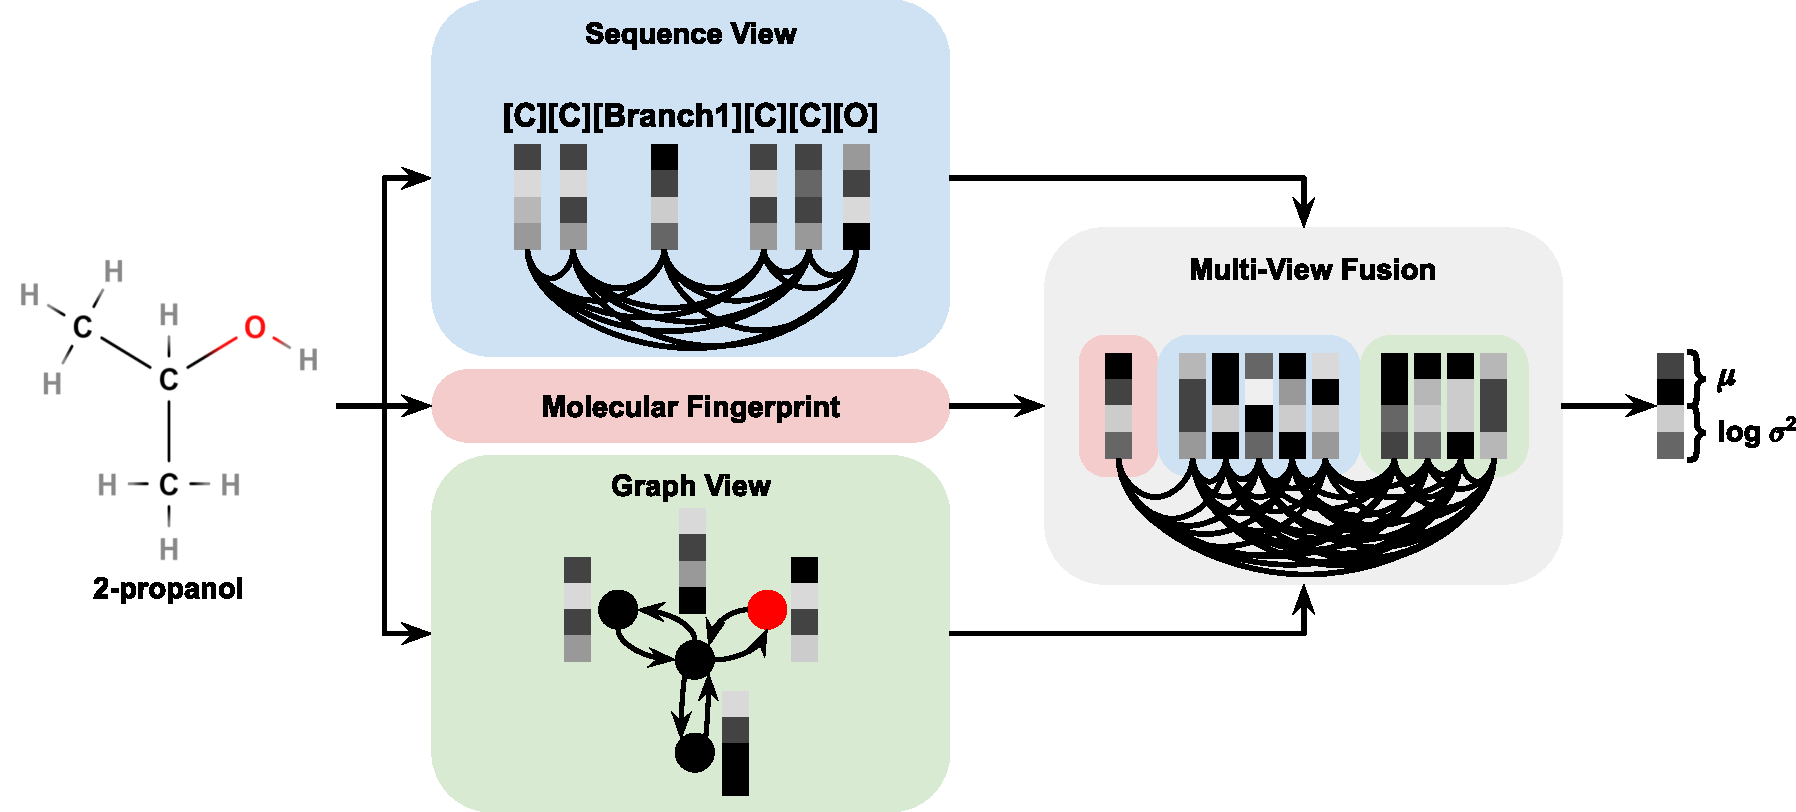
\includegraphics[width=\linewidth]{figs/model/encoder.pdf}
    \caption[Multi-view molecular encoder.]{The multi-view molecular encoder tested in the architectural comparison. The same molecule is read as a token string, a fixed fingerprint vector and an attributed graph. In the graph branch, atoms and bonds are processed by three residual GATv2 layers with four attention heads, with bond attributes included in the attention. The sequence and graph branches contribute one representation per token and per atom, respectively, while the fingerprint contributes a single vector regardless of molecular size. Fusion attends over all these representations jointly. Learned view identifiers, shown by the colors, indicate the source of each representation, and the posterior parameters are read from the fingerprint position.}
    \label{fig:sup_encoder}
\end{figure}

\begin{figure}[H]
    \centering
    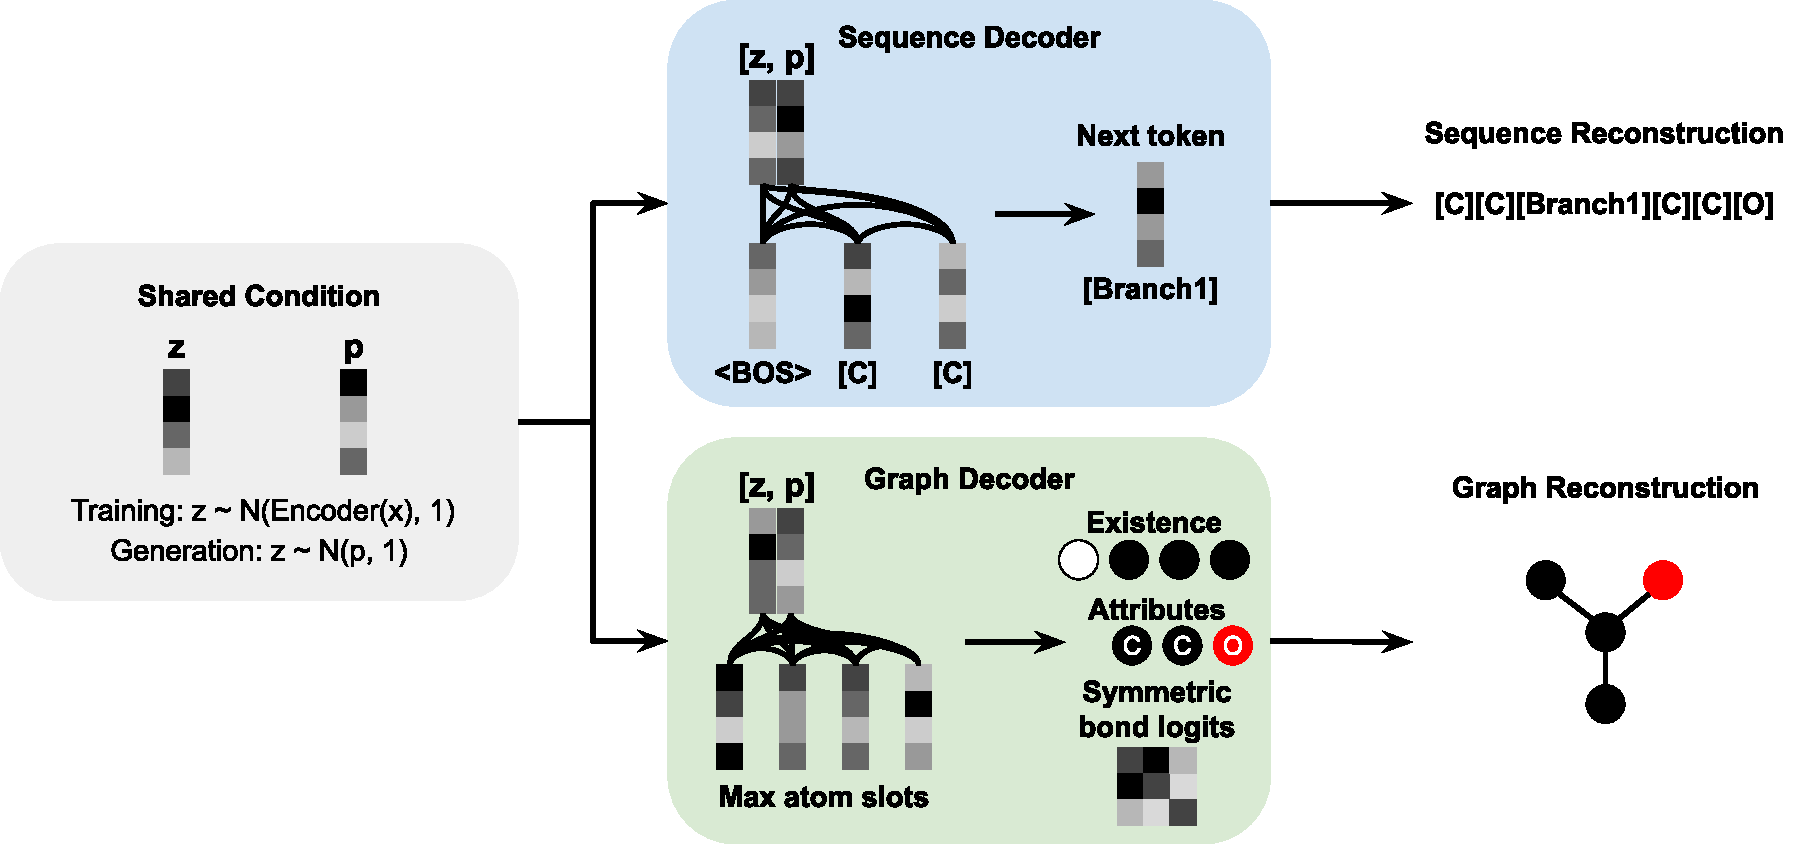
\includegraphics[width=\linewidth]{figs/model/decoder.pdf}
    \caption[Sequence and graph decoders.]{The two alternative decoders. Exactly one is active in each configuration, and both receive the conditioning pair $[z, p]$. The sequence decoder writes the molecular string token by token under causal self-attention. The graph decoder expands the latent representation into a fixed number of learned node queries and processes them through four Transformer layers. It then predicts which nodes exist, their element, chirality and charge, and the bond classes from symmetric low-rank pairwise scores between node representations. During training, $z$ is sampled around the molecular posterior mean; during generation, it is sampled around the protein representation. The decoder itself is used in the same way in both regimes.}
    \label{fig:sup_decoder}
\end{figure}

\begin{figure}[H]
    \centering
    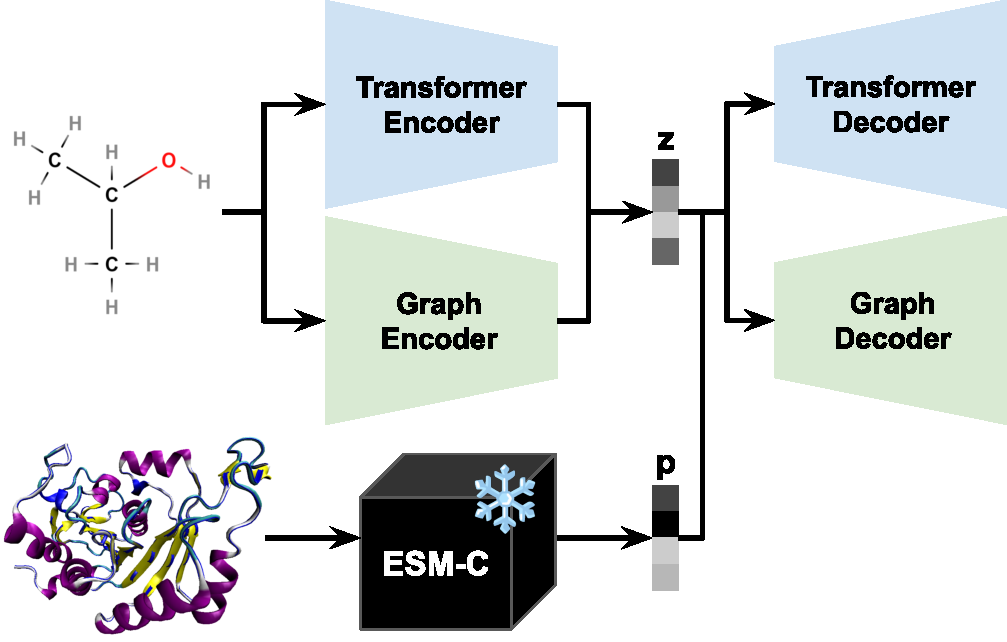
\includegraphics[width=\linewidth]{figs/model/full_model.pdf}
    \caption[The full multi-view architecture.]{The complete architecture with all branches shown: the molecular encoder branches, the frozen ESM-C protein encoder producing $p$, and the two alternative decoders. Each tested configuration uses a subset of these components. The fingerprint branch is always present, the sequence and graph encoder branches are optional, and exactly one decoder is trained at a time.}
    \label{fig:sup_model}
\end{figure}

\begin{table}[H]
    \centering
    \caption[Architectural configurations.]{The six architectural configurations compared in this section. A tick marks an encoder branch that is present. Every configuration includes the fingerprint and at least one of the sequence and graph views of the same molecule, paired with one decoder. Adding encoder branches provides more views at a higher parameter cost. Table \ref{tab:e2_branches} reports the results.}
    \label{tab:configurations}
    \begin{tabular}{lcccc}
        \toprule
        & \multicolumn{3}{c}{\textbf{Encoder branches}} & \\
        \cmidrule(lr){2-4}
        \textbf{Configuration} & \textbf{Fingerprint} & \textbf{Sequence} & \textbf{Graph} & \textbf{Decoder} \\
        \midrule
        Sequence $\rightarrow$ Sequence & \checkmark & \checkmark & - & Sequence \\
        Graph $\rightarrow$ Sequence & \checkmark & - & \checkmark & Sequence \\
        Both $\rightarrow$ Sequence & \checkmark & \checkmark & \checkmark & Sequence \\
        \midrule
        Sequence $\rightarrow$ Graph & \checkmark & \checkmark & - & Graph \\
        Graph $\rightarrow$ Graph & \checkmark & - & \checkmark & Graph \\
        Both $\rightarrow$ Graph & \checkmark & \checkmark & \checkmark & Graph \\
        \bottomrule
    \end{tabular}
\end{table}

\subsubsection*{Auto-encoder branches}\label{sec:branches}
Table \ref{tab:e2_branches} compares the configurations on KIBA using Effective $\Delta$, the model-selection criterion defined in Chapter \ref{sec:metrics}. Pairwise comparisons used Tukey's honestly significant difference procedure \parencite{tukey1949comparing}, with random seed as a blocking factor. Configurations that share a Tukey group did not differ significantly in this metric. Sharing a group therefore means that the experiment did not distinguish their performance, rather than that their performance is necessarily identical.

\begin{table}[H]
    \centering
    \caption[Effective $\Delta$ by encoder and decoder branch.]{Effective $\Delta$ on KIBA for the architectural configurations in Table \ref{tab:configurations}. Configurations sharing a letter in the Tukey group column did not differ significantly under Tukey's honestly significant difference test. The groups separate according to decoder choice: all sequence-decoded configurations belong to group a, and all graph-decoded configurations belong to group b.}
    \label{tab:e2_branches}
    \begin{tabular}{lcc}
        \toprule
        \textbf{Configuration} & \textbf{Effective $\Delta$} & \textbf{Tukey group} \\
        \midrule
        Sequence $\rightarrow$ Sequence & $0.1152 \pm 0.0327$ & a \\
        Graph $\rightarrow$ Sequence & $0.1139 \pm 0.0337$ & a \\
        Both $\rightarrow$ Sequence & $0.1124 \pm 0.0354$ & a \\
        Both $\rightarrow$ Graph & $0.0023 \pm 0.0021$ & b \\
        Graph $\rightarrow$ Graph & $0.0016 \pm 0.0020$ & b \\
        Sequence $\rightarrow$ Graph & $0.0013 \pm 0.0018$ & b \\
        \bottomrule
    \end{tabular}
\end{table}

The main separation is between decoders. Every configuration using sequence decoding obtained a higher Effective $\Delta$ than every configuration using graph decoding, and the two sets formed distinct Tukey groups. Within either decoder group, changing the encoder views produced no statistically significant difference. Thus, the experiment supports the choice of the sequence decoder, while providing no evidence that adding the graph view improves this model's performance.

The configuration ``$\text{Sequence} \rightarrow \text{Sequence}$'' was therefore adopted for SelVAEGen. It retains the fingerprint and sequence encoder branches and uses the sequence decoder. Its result is in the highest-performing group, and adding the graph branch would increase the architecture's complexity without a demonstrated gain in Effective $\Delta$.

\newpage
\clearpage
{
    \setstretch{0.5}
    \printbibliography[heading=secbib, title={References}]
}

\end{document}
